%\documentclass[12pt,twoside]{report}
%cambia qualcosa da twoside a oneside????
\documentclass[12pt, english, makeidx, a4paper, titlepage, oneside]{report}

%\documentclass[12pt,openright]{report}
\usepackage{array}
\usepackage{mathtools}
\usepackage{makeidx}
%\usepackage[italian]{babel}
\usepackage[english]{babel}         %  Package con le regole di sillabazione (italiano)
\usepackage{toptesi}                %  File di stile per le tesi, by CB
\usepackage{epstopdf}
\usepackage[latin1]{inputenc}       %  Per usare i font nuovi
\usepackage{graphicx}               %  Pacchetto per l'inserzione di figure post-script
\usepackage{subfigure}              %  Per mettere piu` immagini una accanto all'altra
\usepackage{booktabs}               
\usepackage{amsfonts}               %  Pacchetto speciale per i font matematici AMS
\usepackage{amssymb}                %  Pacchetto speciale per i simboli matematici AMS
\usepackage{amsmath} 
\usepackage{colortbl}
\usepackage{color}
\usepackage[dvipsnames]{xcolor}
\usepackage{rotating} 
\usepackage{xcolor}
\usepackage{bm}                     %  Il modo per realizzare simboli matematici in neretto
\usepackage{listings}               %  Per includere in modo semplice i listati in appendice
\usepackage{hyperref}
\usepackage{setspace}
\usepackage{etoolbox}% http://ctan.org/pkg/etoolbox
\makeatletter
\patchcmd{\@makechapterhead}{\vspace*{50\p@}}{}{}{}% Removes space above \chapter head
\patchcmd{\@makeschapterhead}{\vspace*{50\p@}}{}{}{}% Removes space above \chapter* head
\makeatother
%\usepackage{titlesec}
%\titleformat{\chapter}[display]
%    {\normalfont\huge\bfseries}{\chaptertitlename\ \thechapter}{20pt}{\Huge}
%\titlespacing*{\chapter}{0pt}{0pt}{40pt}
\usepackage{caption}
\usepackage{float}
\hypersetup{%
    pdfpagemode={UseOutlines},
    bookmarksopen,
    pdfstartview={FitH},
    colorlinks,
    linkcolor={blue},
    citecolor={blue},
    urlcolor={blue}
  }
  

  
  %% Impostazioni per codici VHDL %%
\lstset{basicstyle=\scriptsize\ttfamily, numbersep=2pt, showspaces=false, showstringspaces=false, showtabs=false,frame=\single, breakatwhitespace = true, numbers=left, numberstyle=\tiny, stepnumber=2, numbersep=5pt}
\lstset{backgroundcolor=\color{green!6}}
\lstset{morecomment=[s][\color{blue}]{/*}{*/}}

%% Impostazioni per i i codici MatLab
\lstloadlanguages{Matlab}
\lstset{% general command to set parameter(s)
basicstyle = \scriptsize\ttfamily, % print whole listing small
keywordstyle = \color{blue},% blue keywords
identifierstyle =, % nothing happens
commentstyle = \color{green}, % comments
stringstyle = \ttfamily, % typewriter type for strings
showstringspaces = false, % no special string spaces
firstnumber = 1, % numero della prima linea
numbers = left, %  show number_line
numberstyle = \tiny, % style of number_line
stepnumber = 5, % one number_line after stepnumber
numbersep = 5pt,
language = {Matlab}, % per riconoscere la sintassi matlab
extendedchars = true, % per abilitare caratteri particolari
breaklines = true, % per mandare a capo le righe troppo lunghe
breakautoindent = true, % indenta le righe spezzate
breakindent = 30pt, % indenta le righe di 30pt
}

%% Impostazioni per codici C %%
\lstset{basicstyle=\scriptsize\ttfamily, numbersep=1pt, showspaces=false, showstringspaces=false, showtabs=false,frame=\single, breakatwhitespace = true, numbers=left, numberstyle=\tiny, stepnumber=2, numbersep=5pt}
\lstset{backgroundcolor=\color{green!4}}
\lstset{morecomment=[s][\color{blue}]{/*}{*/}}
\lstset{language=c++, basicstyle=\ttfamily\scriptsize, keywordstyle=\color{blue}, stringstyle=\color{red}, commentstyle=\color{green}\ttfamily}

%listato serve a cambiare la dimensione del carattere nelle appendici con listati
\newenvironment{listato}{\footnotesize}
                        {\normalsize }


%%%%%%%%%%%%%%%%%%%%%%%%%%%%%%%%%%%%%%%%%%%%


%\facolta{Ingegneria dell'Informazione}
\corsodilaurea{Ingegneria Informatica}          % INSERIRE CORSO DI LAUREA

\titolo{Titolo}                           % INSERIRE TITOLO DELLA TESI

\relatore{Prof. Mariagrazia \textsc{Graziano}}                         % INSERIRE IL NOME DEL PRIMO RELATORE
\secondorelatore{Prof. Marco \textsc{Vacca}}                 % INSERIRE IL NOME DEL SECONDO (eventuale) RELATORE
\terzorelatore{Prof. Maurizio \textsc{Zamboni}}                   % INSERIRE IL NOME DEL TERZO (eventuale) RELATORE

\candidata{Gina \textsc{Jiang}}                       % INSERIRE IL NOME DEL PRIMO TESISTA
%\candidata{}                       % INSERIRE IL NOME DELLA PRIMA TESISTA
%\secondocandidato{}                % INSERIRE IL NOME DEL SECONDO (eventuale) TESISTA
               % INSERIRE IL NOME DELLA SECONDA (eventuale) TESISTA
%\terzocandidato{}                  % INSERIRE IL NOME DEL TERZO (eventuale) TESISTA
%\terzacandidata{}                  % INSERIRE IL NOME DELLA TERZA (eventuale) TESISTA
\sedutadilaurea{ 2017}%MODIFICARE IL MESE
\logosede{imm/LogoPoliTo-eps-converted-to}

\setcounter{tocdepth}{4}  %per farlo vedere nel sommario??
\setcounter{secnumdepth}{4} %profondit� delle sottosezioni
\begin{document}
%\inglese\setcaptions
   \frontespizio
\ringraziamenti

%\begin{center}
                           
%\include{new_chapters/sommario}
%\tablespagetrue
\figurespagetrue
                          		% INSERIRE IL NOME DEL FILE CONTENENTE IL SOMMARI
\indici
% L'ELENCO DELLE FIGURE E L'ELENCO DELLE TABELLE VENGONO INSERITI AUTOMATICAMENTE, SE SI VUOLE DISABILITARE QUESTA OPZIONE UTIZZARE I COMANDI \figurespagefalse E \tablespagetrue ALL'INTERNO DEL FILE toptesi.sty. ATTENZIONE I COMANDI SONO GIA' PRESENTI NEL FILE, COMMENTARLI A PIACERE ALL'OCCORRENZA.


%\include{new_chapters/10_fault_analysis}%I need to add this part.

%\doublespacing
\onehalfspacing
%\chapter{Introduction}
The topic discussed in this work of thesis is based on an ASIC (Application-specific integrated circuit) architecture to implement some algorithm regarding the image processing and imange filtering.\\
\section{Advantages of an ASIC based design}
An application-specific integrated circuit (ASIC), is an integrated circuit (IC) customized for a particular use, rather than intended for general-purpose use.\\
The advantages of an ASIC can be divided into four major areas: Unit
cost, performance, power consumption and flexibility. 
\subsection{Unit cost}
One of the biggest advantages of an ASIC based product with respect to a general purpose product is the lower unit cost once a certain
volume has been reached. Unfortunately the volume required to offset
the high NRE costs of an ASIC is very high which means that many
projects are never a candidate for ASICs.\cite{asci0}\\


\subsection{Performance}
Another advantages for using an ASIC is the higher performance. It has been done a comparison of various designs and it was found that an ASIC design was on average 3.2
times faster than an FPGA \cite{asic2}. \\

\subsection{Power consumption}
An ASIC architecture usually has lower power consumption
than a comparable FPGA. 
This is due to the reconfigurability of the FPGA: there is a lot of logic in an FPGA which is used only for configuration.
While the dynamic power consumption of the reconfiguration logic
is practically 0, all of the configuration logic contributes to the leakage
power.\cite{asci0}\\
%\section{ASIC vs General Purpose}

%

\chapter{Integral Image Algorithm}
 The \textit{integral image algorithm}, also known as \textit{summed area table} is a two-dimensional table generated from an input image. Integral image is a very popular and important algorithm in computer vision and computer graphics applications. Especially in real-time computer vision, it is usually used to accelerate calculating the sum of a rectangular area. 
 
  The aim of the IIA is to calculate the sum of values in a rectangular subset of a grid. In particular, the final value of a point inside a grid can be written as:
  
  \begin{equation} \label{eq:IIA eq}
  I(x,y)=\sum\limits_{x'=1}^{x}\sum\limits_{y'=1}^{y}  i(x',y')
  \end{equation}
   
   As shown in the figure \ref{fig:IIA}, the value of the dark blue rectangle can be calculated as the sum of all the light blue rectangles.
   
 
  	\begin{figure}[h]
  		\centering
  	 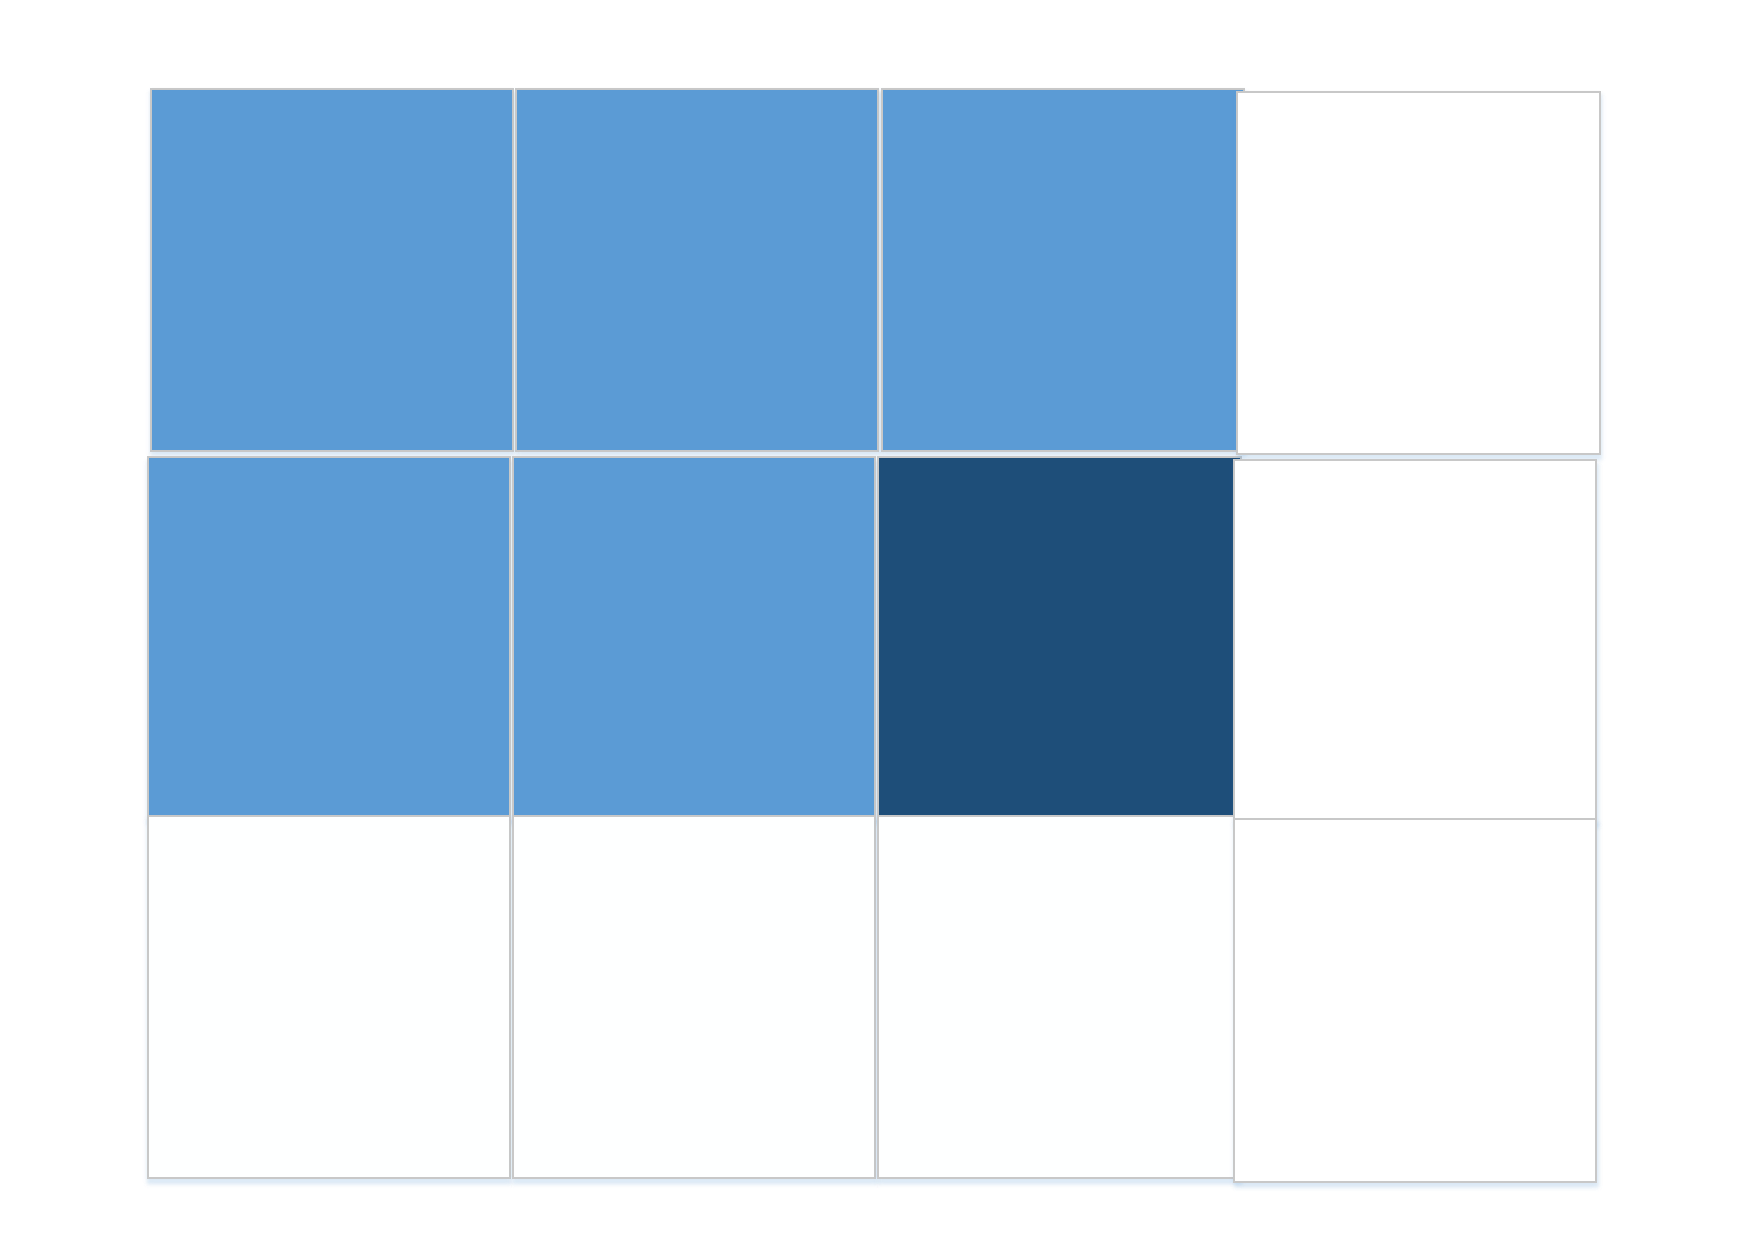
\includegraphics[scale=0.25]{imm/iia/Disegno1}  
   \caption{SAT of a single cell}
   \label{fig:IIA}
\end{figure}
  
 \section{Method used}
 I decided to use the approach ASAP (as soon as possible), so in this implementation we try to maximize the parallelism.
 To better explain, we first look to the Integral Image of a 1D array.
 At each step \textit{i} we have the array  partitioned in array of size $ 2^{i} $, and each of them has its own integral image values.\\
 In the next step \textit{i+1}, we pair two consecutive array of size $ 2^{i} $, (thus having an array of $ 2^{i+1} $) and do the Integral image. \\Since we have already computed the partial integral image, for the new one, the elements from \textit{1} to $ 2^{i} $ has the correct values, while for the elements from $ 2^{i} $ to $ 2^{i+1} $ we need to sum the value stored in position $2^{i} $.
 Figure \ref{fig:iia0} represents this method, while figure \ref{fig:iia1} shows an example of an 8-array.
 
   	\begin{figure}[h]
   		\centering
   		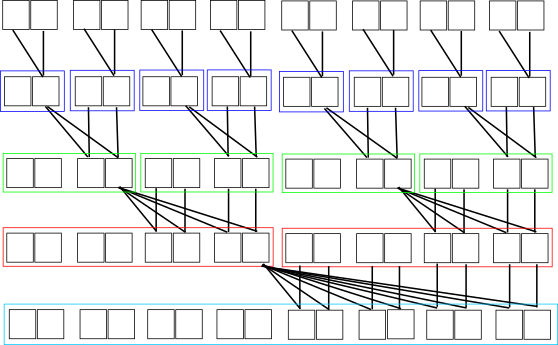
\includegraphics[width=\textwidth]{imm/iia/iia00.png}  
   		\caption{Schematic of the SAT of a 1D array}
   		\label{fig:iia0}
   	\end{figure}
   	
   	  	\begin{figure}[h]
   	  		\centering
   	  		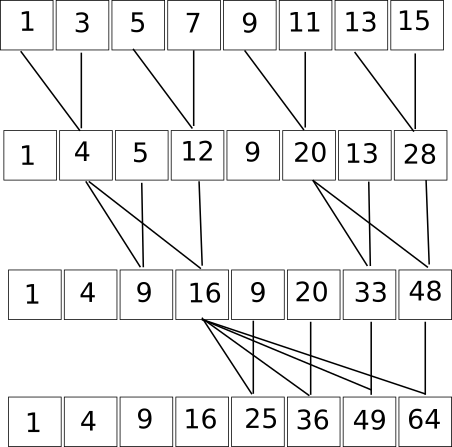
\includegraphics[width=\textwidth]{imm/iia/iia1.png}  
   	  		\caption{SAT of a 1D array with some values}
   	  		\label{fig:iia1}
   	  	\end{figure}
  When we want to handle the integral image of a 2D array, we can compute the same method both vertically and horizontally. 	  	
   	  	\clearpage
  \section{Hardware Implementation} \label{hiiia}
  The algorithm has been properly implemented for an ASIC architecture that privileges the throughput (i.e. computes as fast as possible).
   The pseudocode is the following:
   \begin{enumerate}
   	
   	\item Divide the NxN matrix into small 2x2 matrices and compute the corresponding summed area table (SAT).
   	This step is shown in figures \ref{fig:IIA1} and \ref{fig:IIA1a}
   	
   	  \begin{figure}[h]
   	  	\centering
   	  	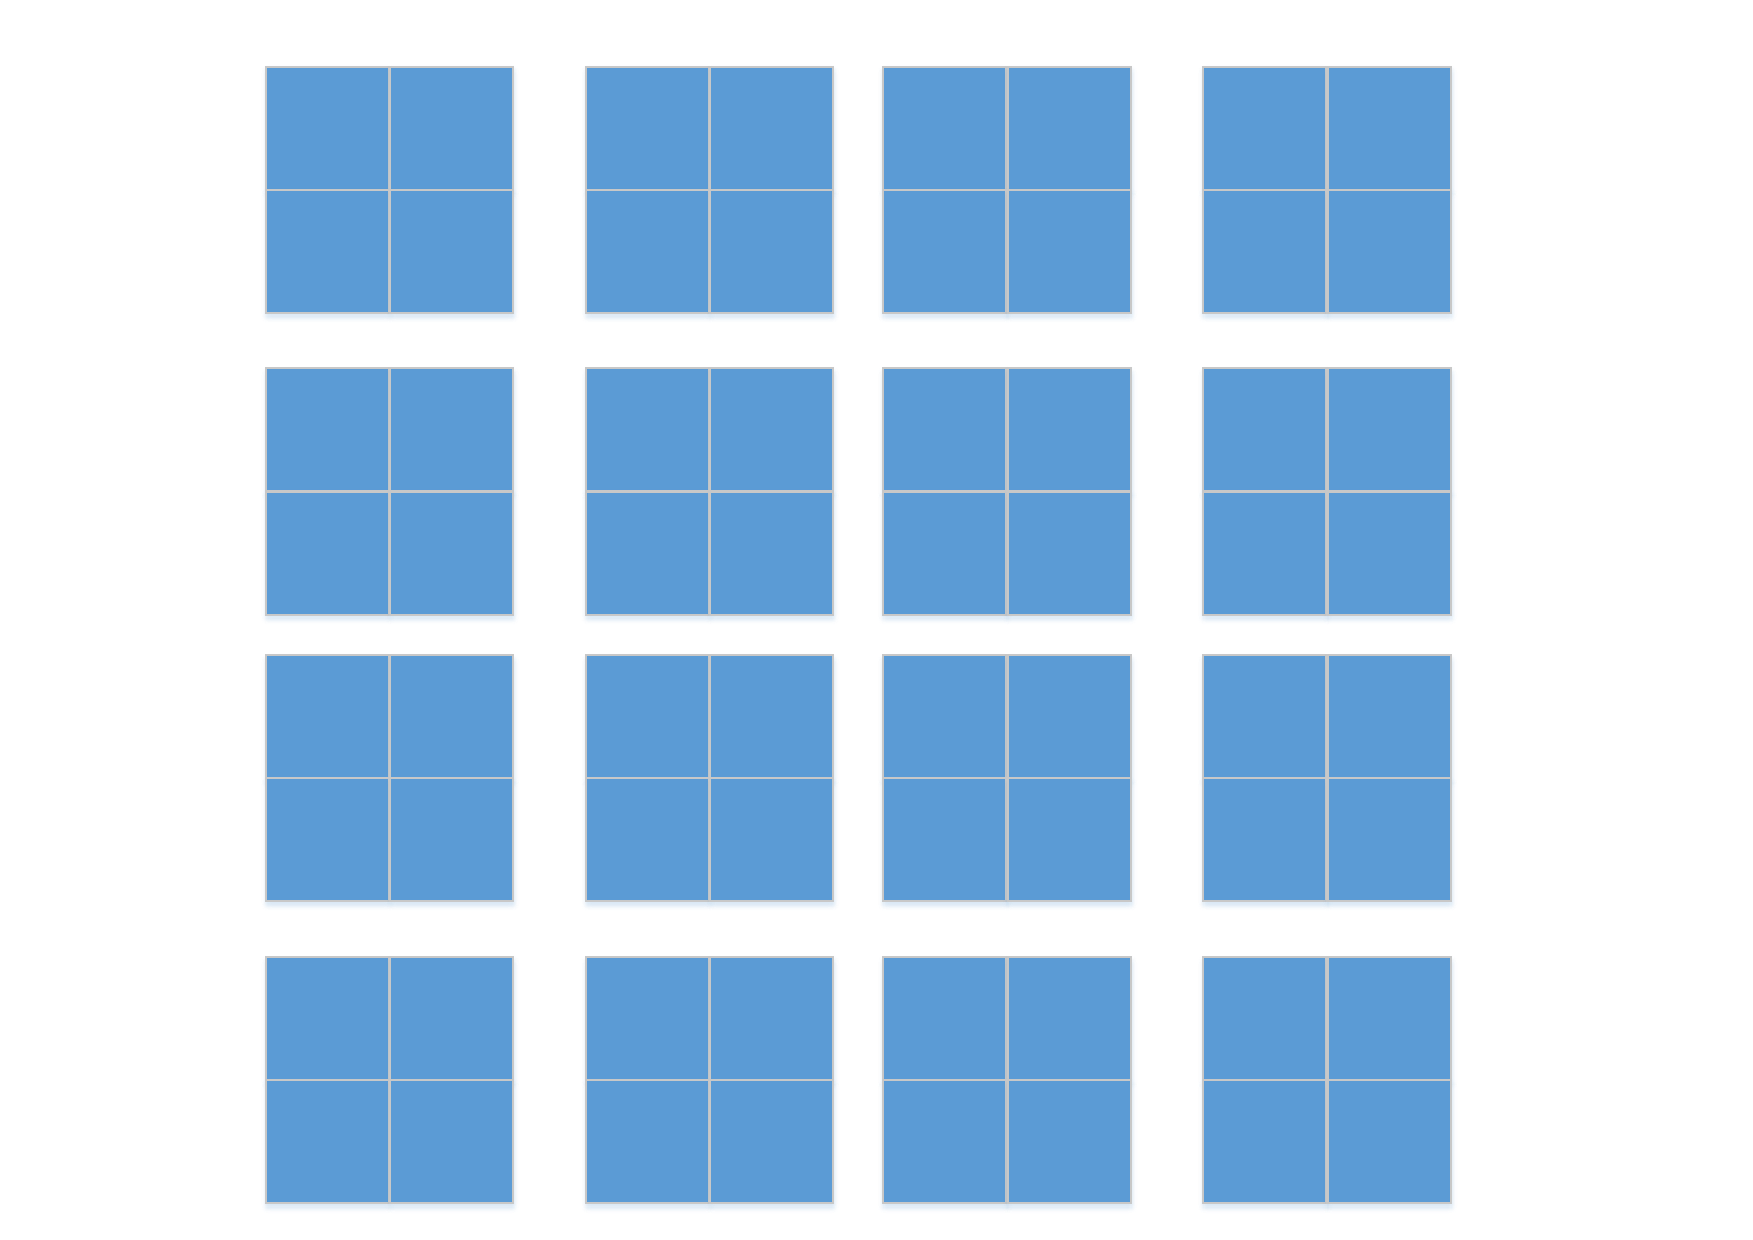
\includegraphics[scale=0.45]{imm/iia/iia_step1}  
   	  	\caption{ Subdivision in 2x2 matrices} 
   	  	\label{fig:IIA1}
   	  \end{figure}
   	
   \begin{figure}[h]
   	\centering
   	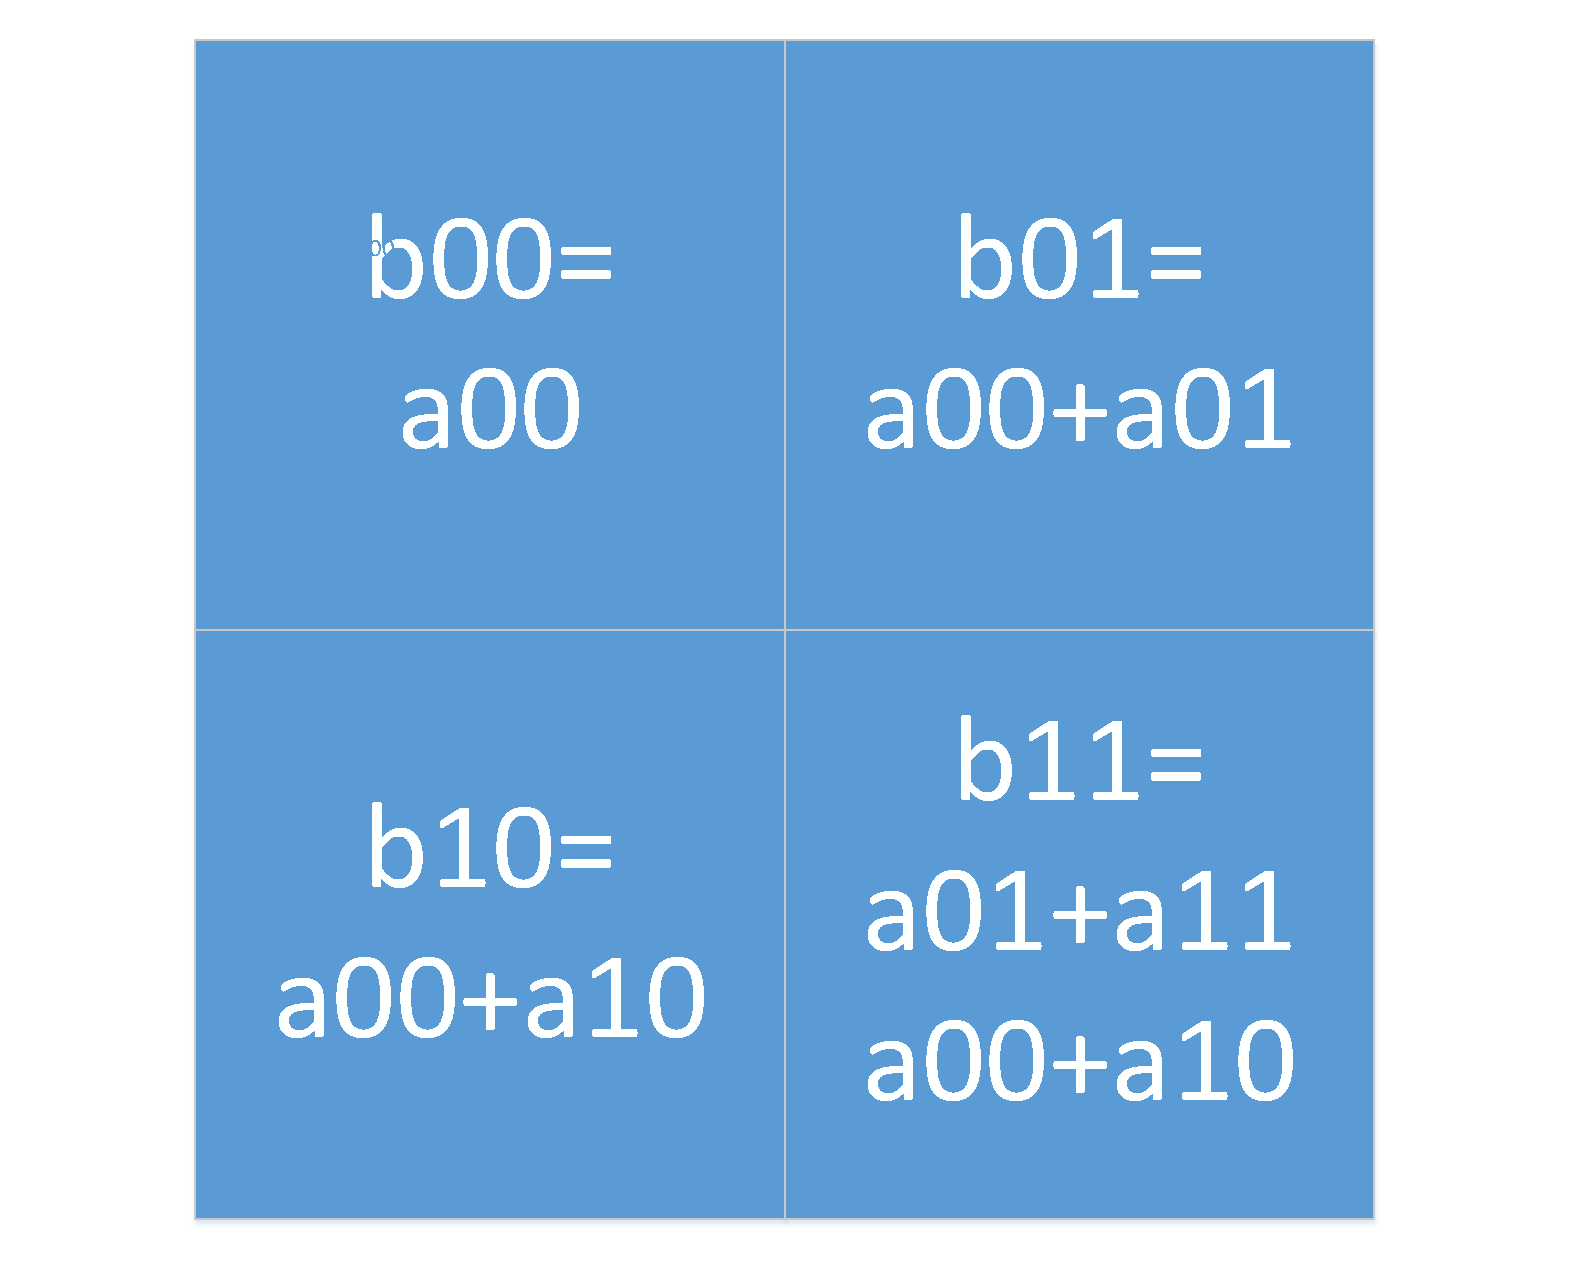
\includegraphics[scale=0.25]{imm/iia/iia_step1a}  
   	\caption{SAT of a 2x2 matrix} 
   	\label{fig:IIA1a}
   \end{figure}
   
 
   
   	\item Group all the above matrices into 4 matrices and evaluate the corresponding SATs.
   	The computation will be faster because we have some partial SATs.
   	When we sum vertically, we just sum to all the lower half cells with the corresponding cell of the last row of the upper half matrix. This is done because the last row of the upper half contains the partial SAT of the small matrices computed in the previous step.
   	Figure \ref{fig:IIA2aa} shows that after this operation the left half side of this 4x4 matrix has its SAT computed.
   	Similarly we sum horizontally: as shown in figure \ref{fig:IIA2b} we add to all cells of the right side the corresponding cell of the last column of the left half matrix. Now all cells of this 4x4 matrix has the SAT computed
   	
   	   \begin{figure}[h]
   	 \centering
   	   	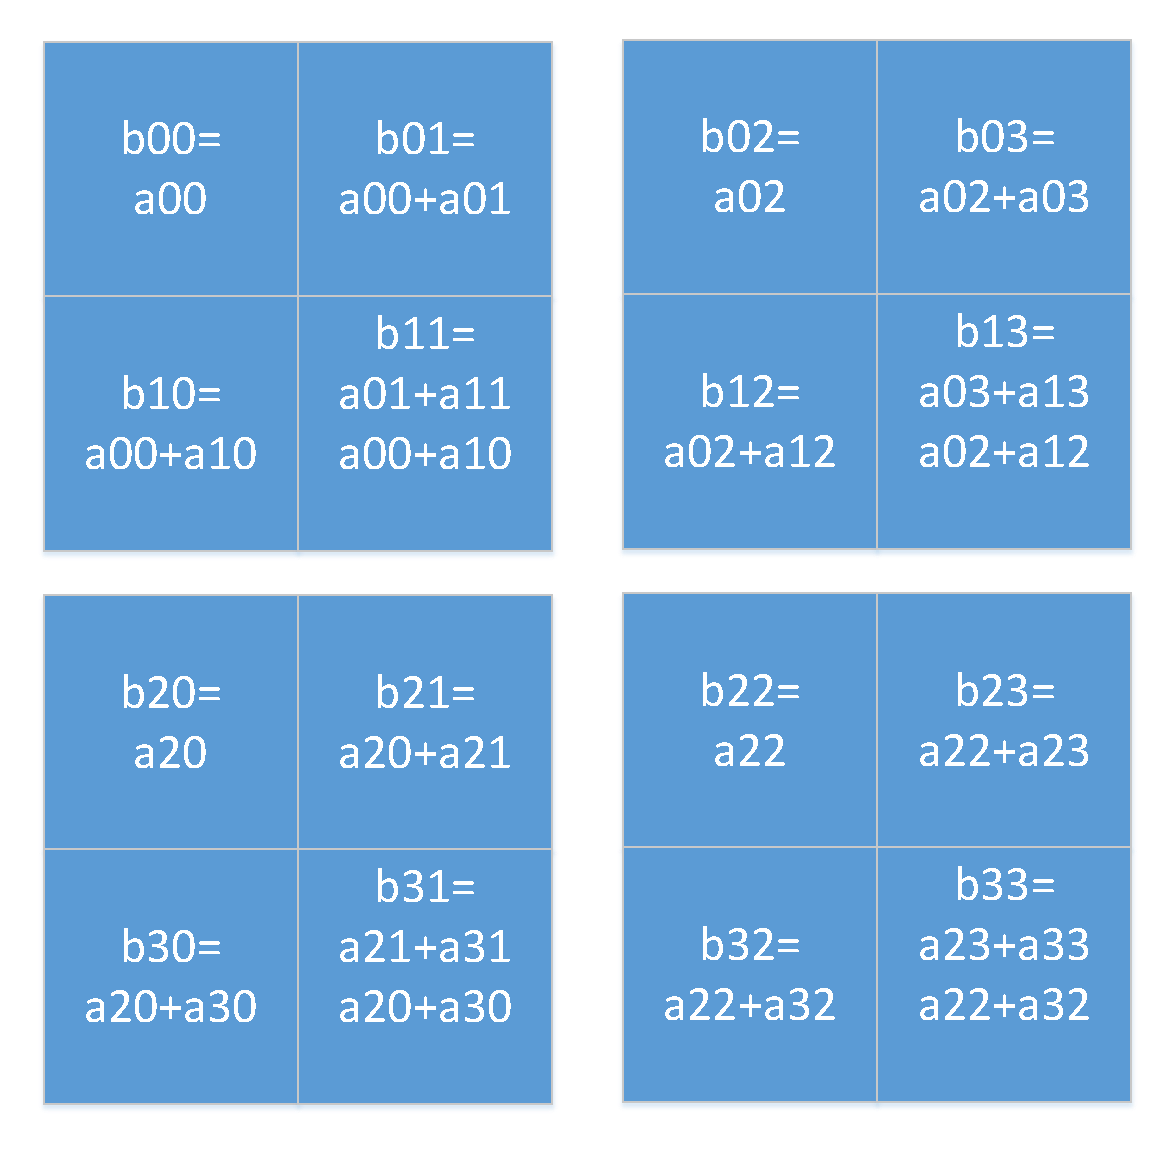
\includegraphics[scale=0.40]{imm/iia/iia_step2a}  
   	   	\caption{Step 2-Initial state of a 4x4 matrix} 
   	   	\label{fig:IIA2a}
   	   \end{figure}
   	   
   	   \begin{figure}[h]
   	   \centering	
   	   	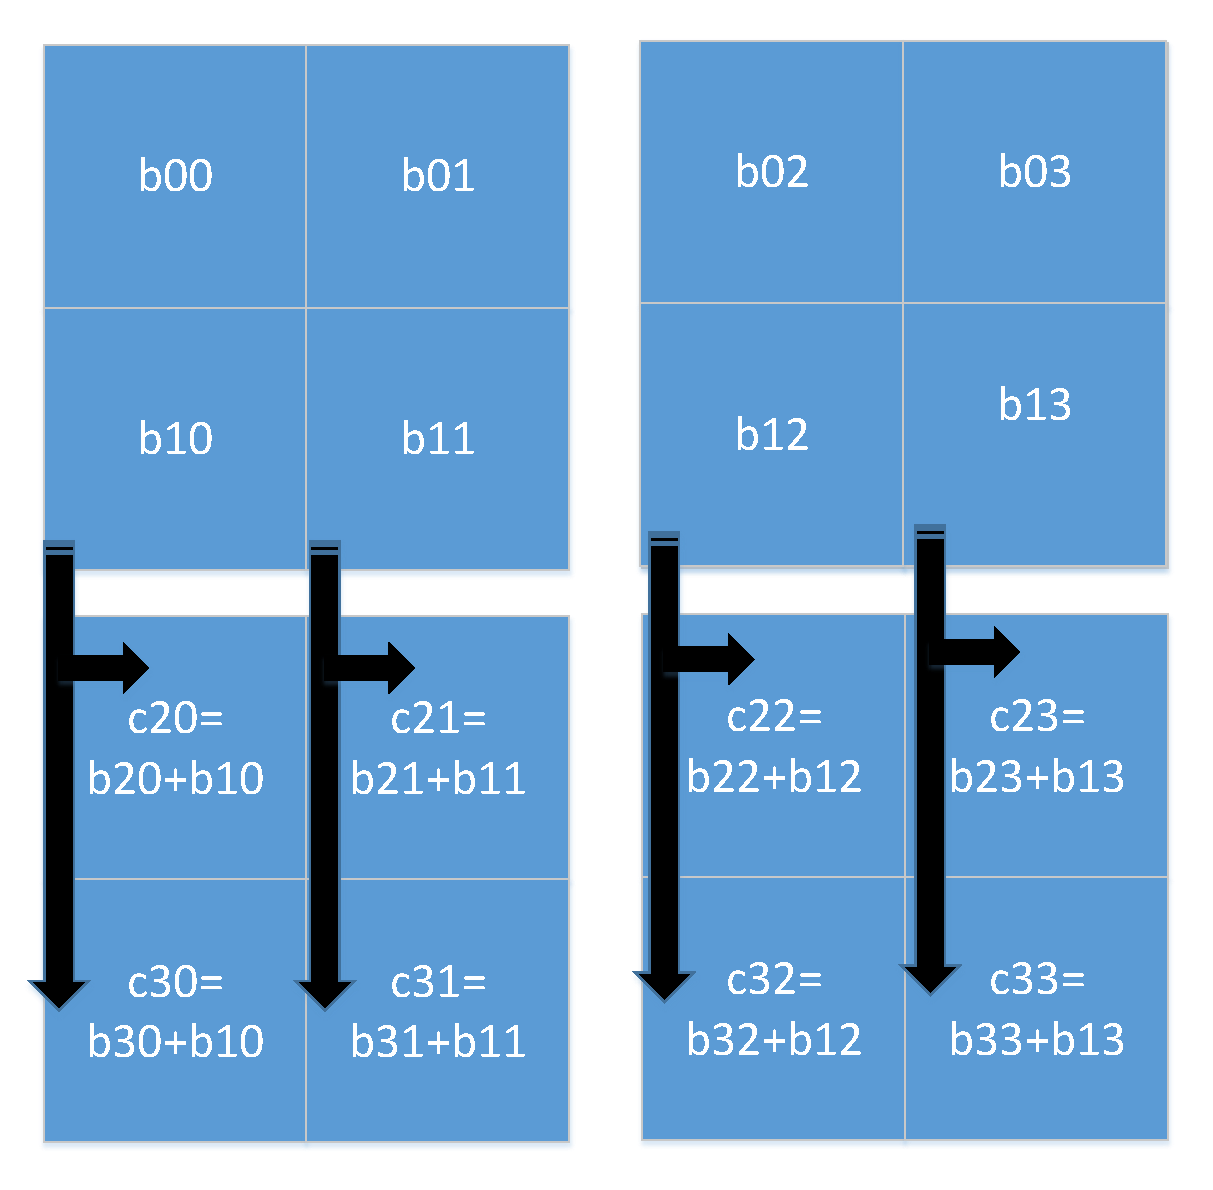
\includegraphics[scale=0.40]{imm/iia/iia_step2aa}  
   	   	\caption{Step 2-Sum vertically.}
   	   	\label{fig:IIA2aa}
   	   \end{figure}
   	   
   	   \begin{figure}[h]
   	   	\centering
   	   	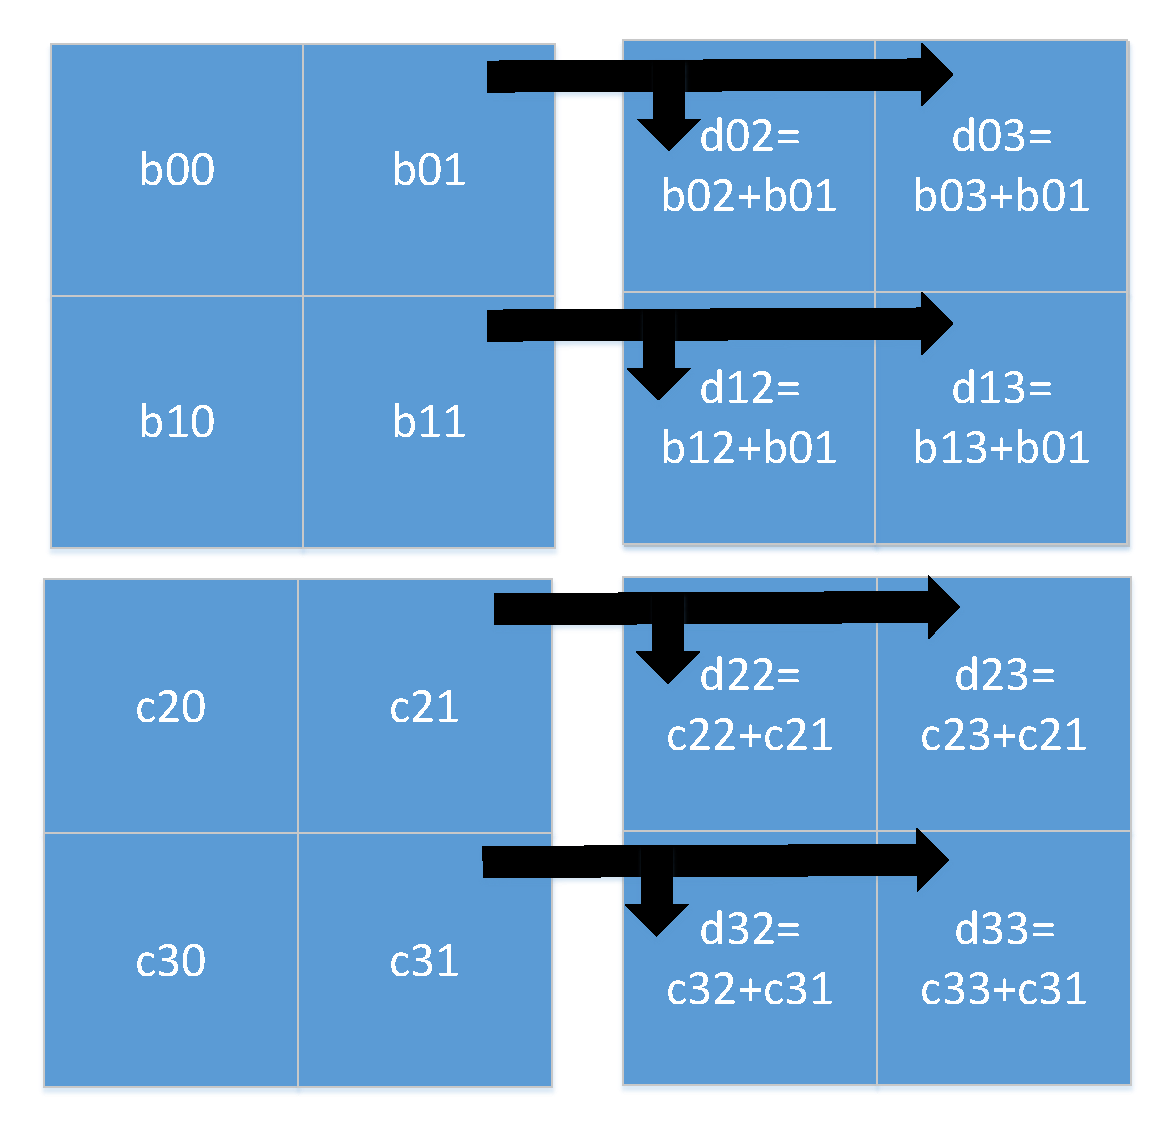
\includegraphics[scale=0.40]{imm/iia/iia_step2b}  
   	   	\caption{Step 2-Sum horizonatlly.} 
   	   	\label{fig:IIA2b}
   	   \end{figure}
  
   
   \item We repeat the prevoius step until we reach the matrix of dimension NxN
    \begin{figure}[h]
    	\centering	
    	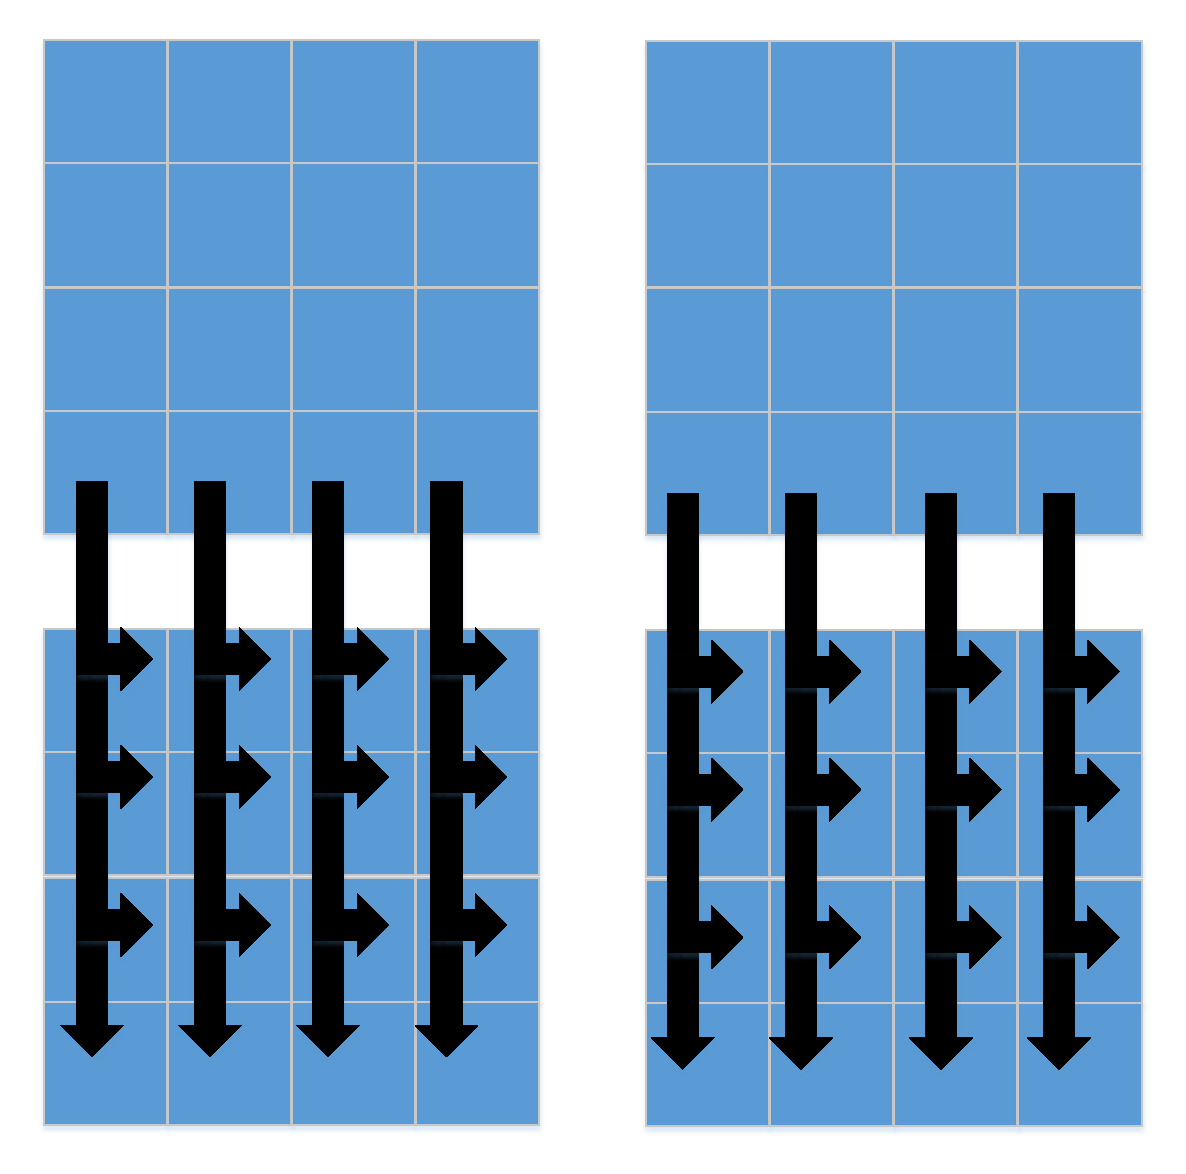
\includegraphics[scale=0.40]{imm/iia/iia_step3a}  
    	\caption{Step 3-Sum vertically.}
    	\label{fig:IIA3a}
    \end{figure}
    
    \begin{figure}[h]
    	\centering
    	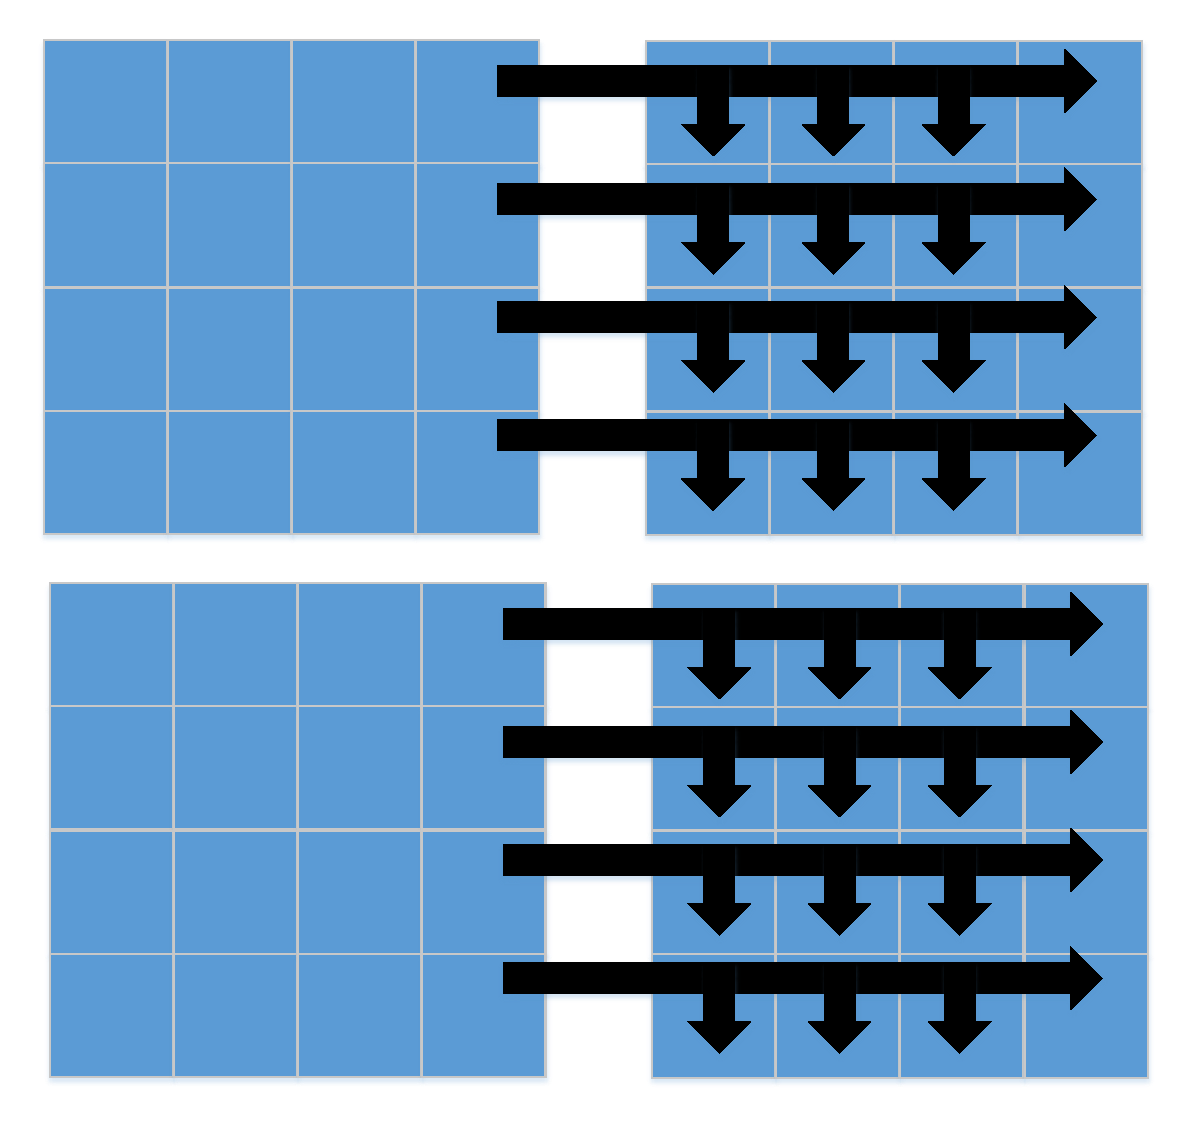
\includegraphics[scale=0.40]{imm/iia/iia_step3b}  
    	\caption{Step 3-Sum horizonatlly.} 
    	\label{fig:IIA3b}
    \end{figure}
     \end{enumerate}
     \clearpage
  \section{Pipelined Implementation}
  As explained before, in every step we divide the original matrix into small matrices of the size $ 2^i $x$ 2^i $ ( $ i $ represent the number of the actual step), and compute the SAT of each matrix independently from one another.
  The computed SATs will be used in the next step to evaluate the SATs of matrices with size $ 2^{i+1} $x$ 2^{i+1} $.
  We repeat this process until we reach the SAT of the original matrix. Figure \ref{fig:IIA_overall} represent the scheme of this implementation for a 8x8 matrix.
  The simbol $ \bigoplus $ means that it will evaluate the SAT of a matrix $ 2^{i+1} $x$ 2^{i+1} $ by using the SATs of 4 matrices $ 2^i $x$ 2^i $.
  By looking to the picture, we can clearly imagine to put some pipeline registers. This is possible because in each step $ i $ we need only the values calculated in the previous step $ i-1 $, we don't need the other values found in the other steps.
   
     \begin{figure}[h!]
     	\centering
     	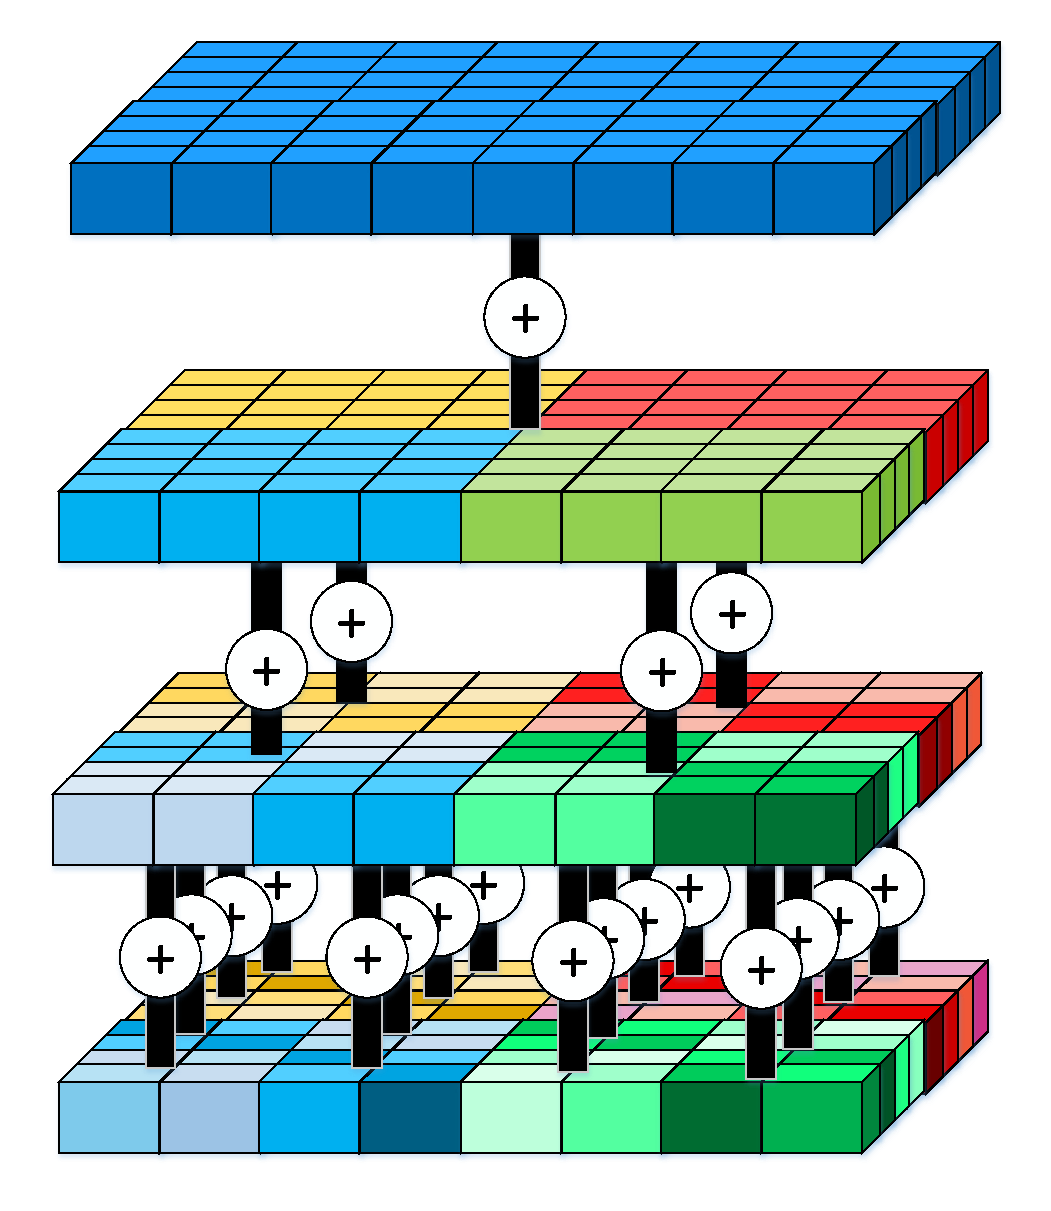
\includegraphics[scale=0.9]{imm/iia/iia_overall}  
     	\caption{Scheme of the SAT algorithm's imlementation.} 
     	\label{fig:IIA_overall}
     \end{figure}
     \clearpage
     \section{Simulation and Test}
     I did some tests of this implementation with different size and dimension. In the fig.\ref{fig:tb_iia} we can see the results of a matrix 4x4.
     
     \begin{figure}[h!]
     	\centering	
     	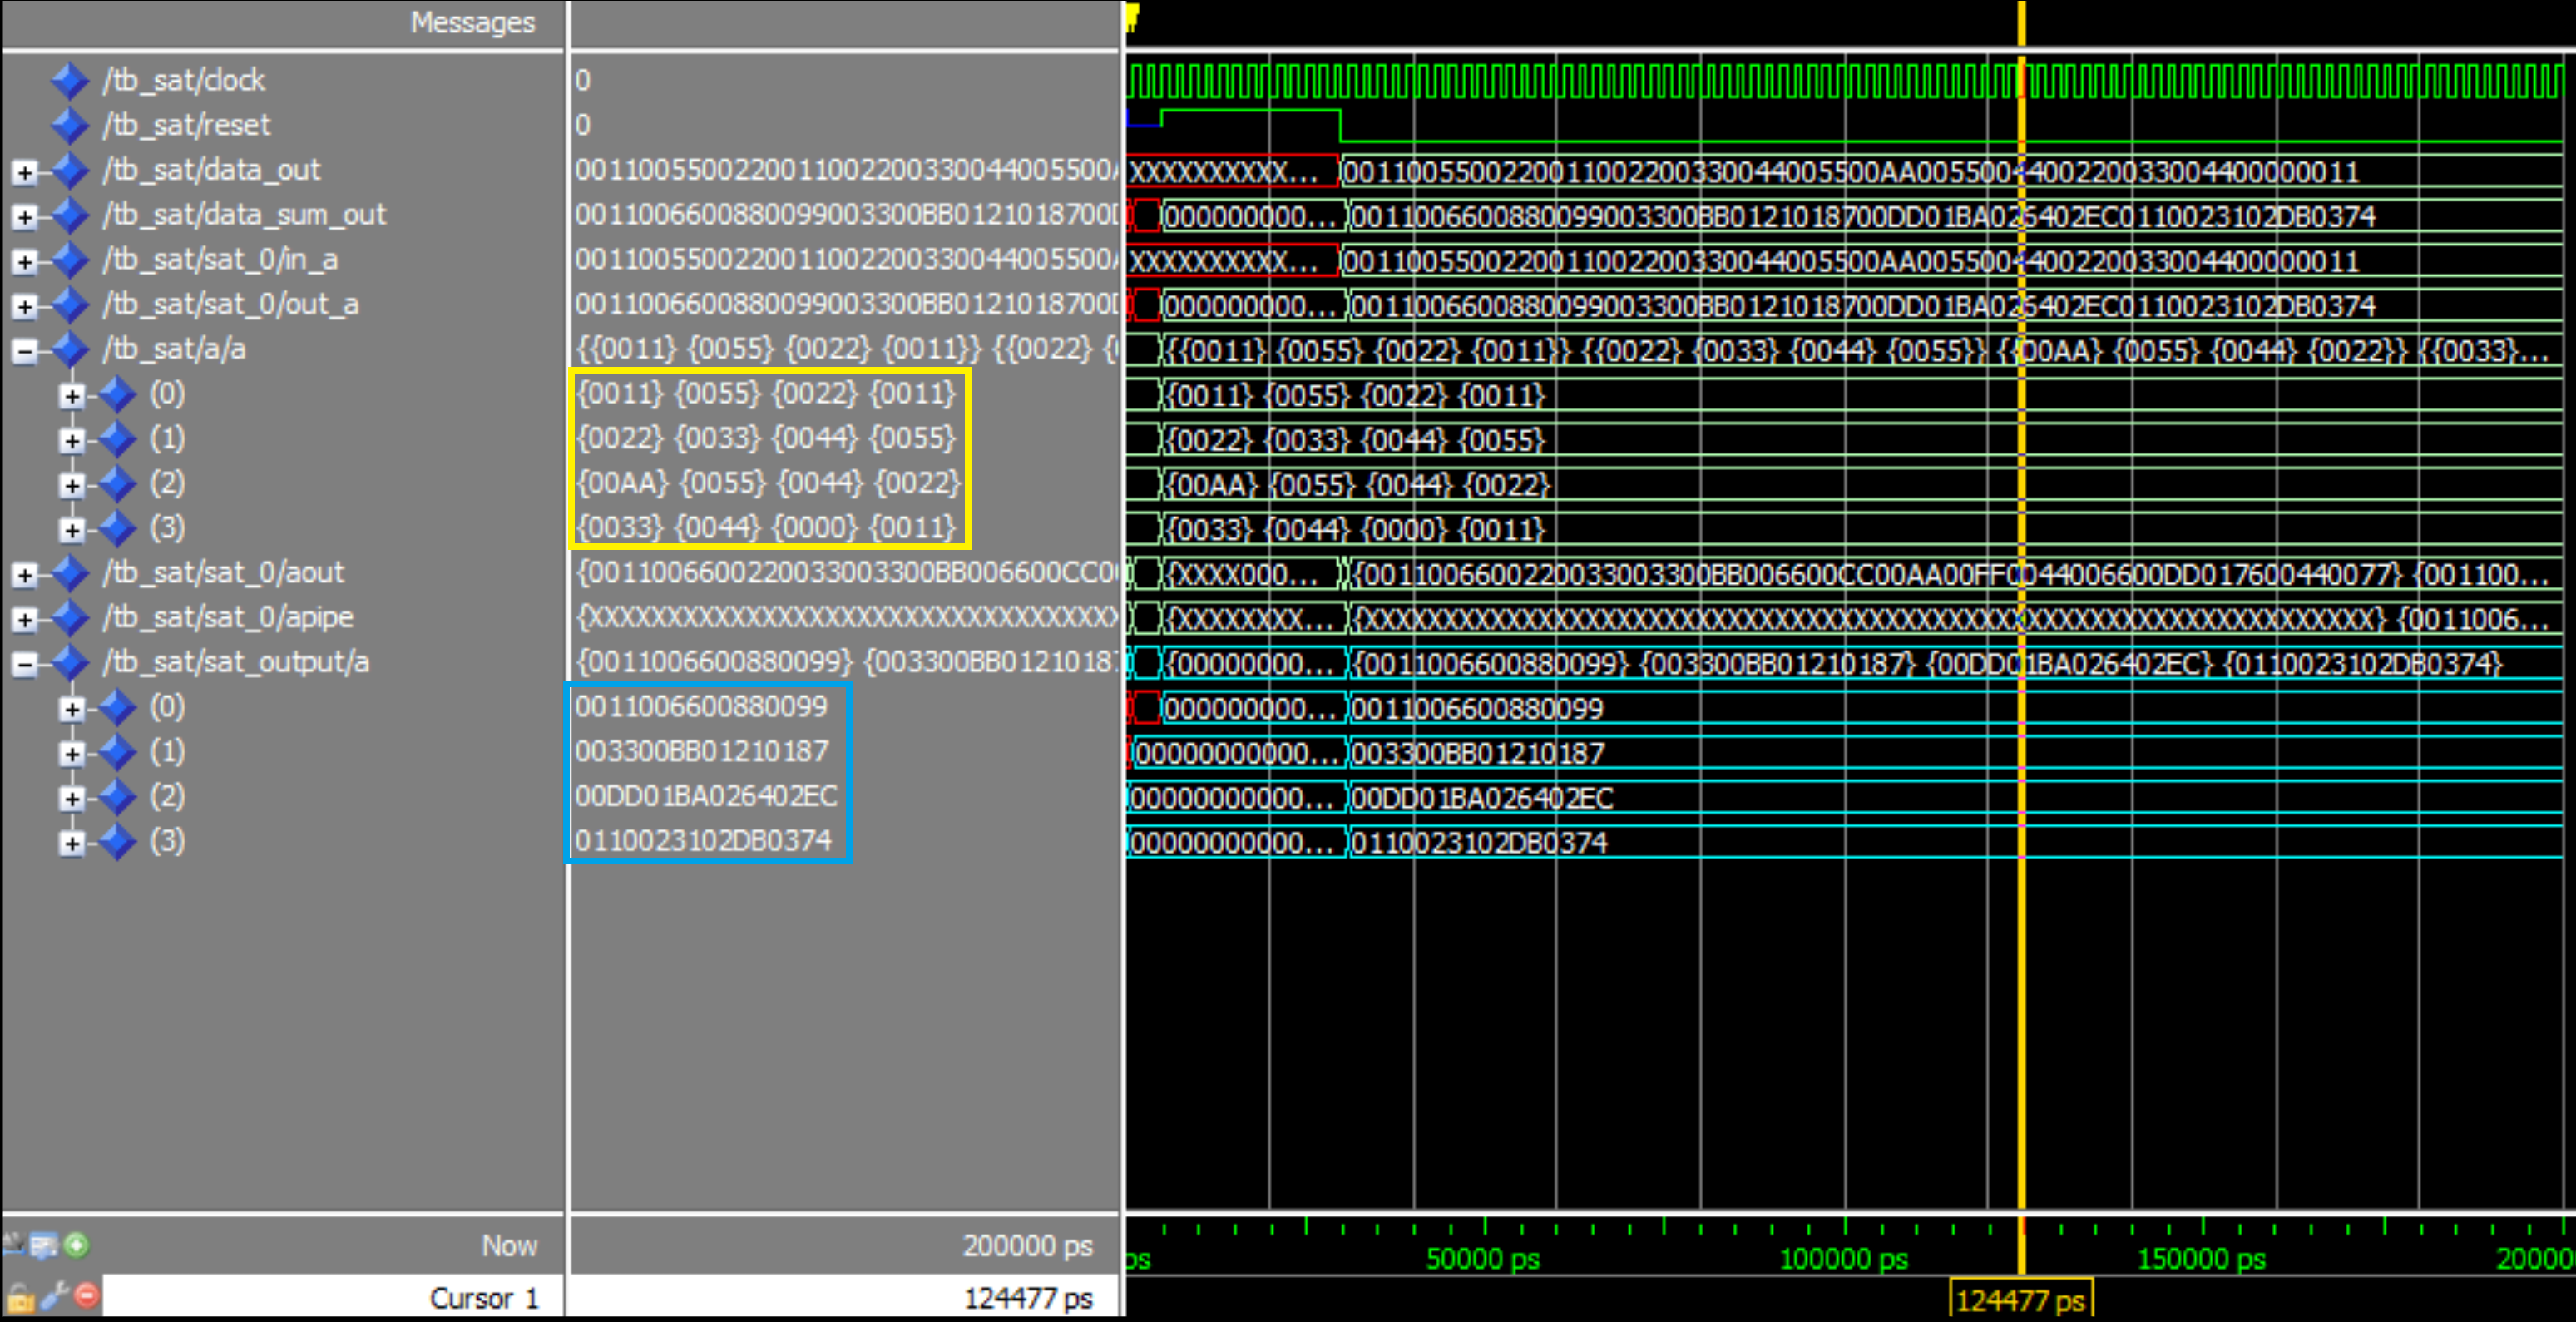
\includegraphics[width=\textwidth]{imm/iia/wave1.png}  
     	\caption{Integral Image-Results of the simulation} 
     	\label{fig:tb_iia}
     \end{figure}
     
     The input matrix is the one highlighted in yellow, while the output matrix is highlighted in light blue.
     We start from these values \begin{center}
     	$ 
     	\begin{bmatrix}
     	0x11 & 0x55 & 0x22 & 0x11\\
     	0x22 & 0x33 & 0x44 & 0x55   	\\
     	0xAA&0x55 & 0x44  &  0x22 \\
     	0x33& 0x44 & 0x0 & 0x11
     	\end{bmatrix}= 	\begin{bmatrix}
     	17 &   85 &   34 &   17\\
     	34  &  51  &  68  &  85\\
     	170  &  85  &  68  &  34\\
     	51    &68    & 0    &17\end{bmatrix}$
     \end{center}
     \bigskip
     we partition the original matrix in matrices 2x2
     \begin{center}
     	$ 
     	\begin{bmatrix}
     	\begin{pmatrix}
     	0x11 & 0x55\\
     	0x22 & 0x33
     	\end{pmatrix}&
     	\begin{pmatrix}
     	0x22 & 0x11\\
     	0x44 & 0x55 
     	\end{pmatrix}\\
     	&\\
     	\begin{pmatrix}
     	0xAA&0x55\\
     	0x33& 0x44
     	\end{pmatrix}&
     	\begin{pmatrix}
     	0x44  &  0x22\\
     	0x0 & 0x11
     	\end{pmatrix}
     	\end{bmatrix}
     =\begin{bmatrix}
     \begin{pmatrix}
     17 &85\\
      34& 51
     \end{pmatrix}&
     \begin{pmatrix}
     34 & 17\\
     68& 85 
     \end{pmatrix}\\
     &\\
     \begin{pmatrix}
     170&85\\
     51&68
     \end{pmatrix}&
     \begin{pmatrix}
     68  &34\\
     0 & 17
     \end{pmatrix}
     	\end{bmatrix}$
     \end{center}\bigskip
      and we perform the summed area table for each matrix 2x2
      \begin{center}
      	$ \begin{bmatrix}
      	\begin{pmatrix}
      	17 &17+85\\
      	34+17& 51+17+85+34
      	\end{pmatrix}&
      	\begin{pmatrix}
      	34 & 17+34\\
      	68+34& 85+17+34+68 
      	\end{pmatrix}\\
      	&\\
      	\begin{pmatrix}
      	170&85+170\\
      	51+170&68+170+85+51
      	\end{pmatrix}&
      	\begin{pmatrix}
      	68  &34+68\\
      	0+68 & 17+68+34
      	\end{pmatrix}
      	\end{bmatrix} =$
      \end{center}\bigskip
      \begin{center}
      	$\begin{bmatrix}
      	\begin{pmatrix}
      	17 &102\\
      	51& 187
      	\end{pmatrix}&
      	\begin{pmatrix}
      	34 & 51\\
      	102& 204 
      	\end{pmatrix}\\
      	&\\
      	\begin{pmatrix}
      	170&255\\
      	221&374
      	\end{pmatrix}&
      	\begin{pmatrix}
      	68  &102\\
      	68 & 119
      	\end{pmatrix}
      	\end{bmatrix}$
      \end{center}
      \bigskip
      If we translate it in hexdecimal we get
      \begin{center} \label{iia_matrix}
      	$ \begin{bmatrix}
      	\begin{pmatrix}
      	0x11 &0x66\\
      	0x33& 0xBB
      	\end{pmatrix}&
      	\begin{pmatrix}
      	0x22 & 0x33\\
      	0x66& 0xCC 
      	\end{pmatrix}\\
      	&\\
      	\begin{pmatrix}
      	0xAA&0xFF\\
      	0xDD&0x176
      	\end{pmatrix}&
      	\begin{pmatrix}
      	0x44  &0x66\\
      	0x44 &0x77
      	\end{pmatrix}
      	\end{bmatrix} $
      \end{center}
      \bigskip
      If we look the signal $ aout $ on the fig \ref{fig:tb_iia}, we can see the partial summed area table.
      \begin{center}
      	$ aout=0x0011006600220033003300BB006600CC00AA00FF0044006600DD017600440077 $
      \end{center}
      we know that each row has 4 elements of 16 bits
      \begin{center}
      	$ \begin{bmatrix}
      	1^{st}row=0x0011006600220033\\
      	2^{nd}row=0x003300BB006600CC\\
      	3^{rd}row=0x00AA00FF00440066\\
      	4^{th}row=0x00DD017600440077
      	\end{bmatrix} =\begin{bmatrix}
      	0x11 &0x66 & 0x22 & 0x33\\
      	0x33 & 0xBB &0x66&0xCC\\
      	0xAA&0xFF&0x44&0x66\\
      	0xDD&0x176&0x44&0x77
      	\end{bmatrix}$
      \end{center}
      which is the same we obtained above.\\
      Now we have to evaluate the summed area table of the matrix 4x4 by using the partial sum we have just found.
      As described before (section \ref{hiiia}), when we sum vertically, we sum to all the lower half cells with the corresponding cell of the last row of the upper half matrix. Similarly we sum horizontally
      \begin{center}
      	$  \begin{matrix}
      	
      	\begin{bmatrix}
      	17 &102 & 34 & 51\\
      	51 &187 &102&204\\
      	170&255&68&102\\
      	221&374&68&119
      	\end{bmatrix}\\
      	\Downarrow\\
       	\end{matrix}$\\
       	sum vertically\\
       	$ \Downarrow $\\
       	$\begin{matrix}
       	
      	\begin{bmatrix}
      	17 &102 & 34 & 51\\
      	51 &187 &102&204\\
      	170+51&255+187&68+102&102+204\\
      	221+51&374+187&68+102&119+204
      	\end{bmatrix}
      	\\\Downarrow
      	\end{matrix}$\\
      	sum horizontally\\
      	$ \Downarrow $\\$
      	\begin{bmatrix}
      	17 &102 & 34+102 & 51+102\\
      	51 &187 &102+187&204+187\\
      	221&442&170+442&306+442\\
      	272&561&170+561&323+561
      	\end{bmatrix}$
      \end{center}
      \bigskip
      Finally we get        
     \begin{center}
     	$ \begin{bmatrix}
     	17&   102&   136&   153\\
     	51 &  187 &  289 &  391\\
     	221  & 442  & 612  & 748\\
     	272   &561   &731   &884\\
     	\end{bmatrix}=
     	\begin{bmatrix}
     	0x11 & 0x66 & 0x88 & 0x99\\
     	0x33 & 0xBB & 0x121 & 0x187   	\\
     	0xDD&0x1BA & 0x264  &  0x2EC \\
     	0x110& 0x231 & 0x2DB & 0x374
     	\end{bmatrix}$
     \end{center}
     Which is the same result given in the simulation (fig \ref{fig:tb_iia}, signal $ sat\_output/a $) and also by MATLAB as shown below
      \begin{figure}[h!]
      	\centering	
      	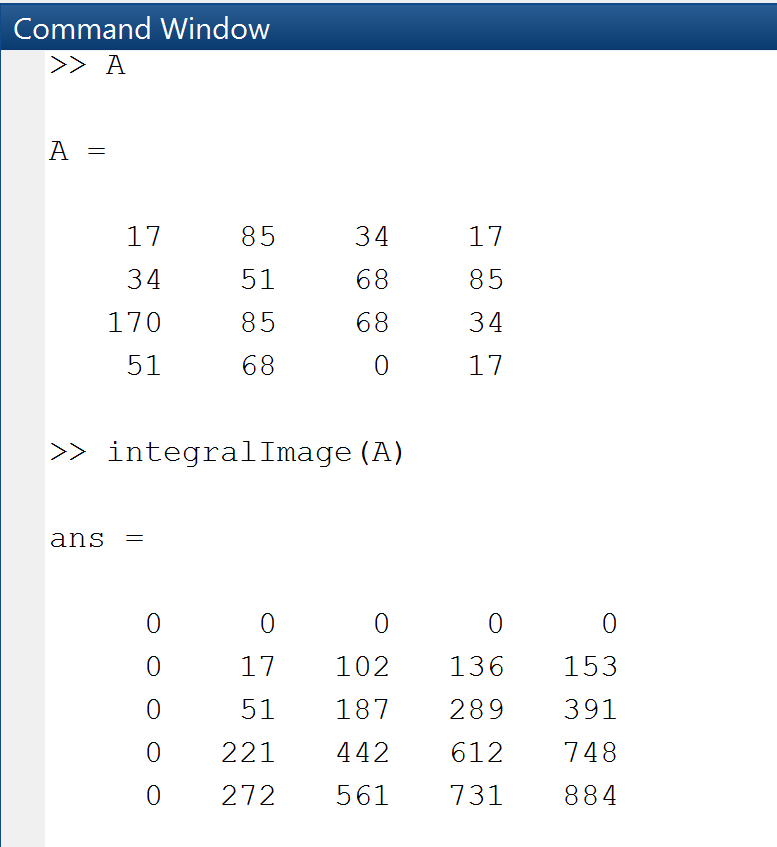
\includegraphics[width=0.8\textwidth]{imm/iia/iia_mat.png}  
      	\caption{Integral Image-Checking with MATLAB} 
      	\label{fig:iia_mat}
      \end{figure}
 \clearpage
 \section{Comparison}
 There are two typical existed image integral algorithms on GPUs. The first is the Inclusive Scan algorithm. The second is the Balanced Trees Parallel Scan algorithm. Compared with the Inclusive Scan algorithm, the proposed scheme reduces logarithmically the global computation time without any pipeline (with pipeline, the improvement will be even greater). Compared with the Balanced Trees Parallel Scan algorithm, the proposed algorithm only needs about half of the global computation time.
 The theoretical implementation shows that the proposed algorithm gets the best performance compared with the two above integral algorithms.
 
 
 \subsection{Inclusive Scan algorithm}
 We perform the inclusive scan for each row and evaluate the partial sum.
 Finally we perform the inclusive scan for each column.
 Figure \ref{fig:inclusive_scan} shows an example of this implementation for a matrix 3x3. \cite{sat3}
 
   \begin{figure}[h!]
   	\centering
   	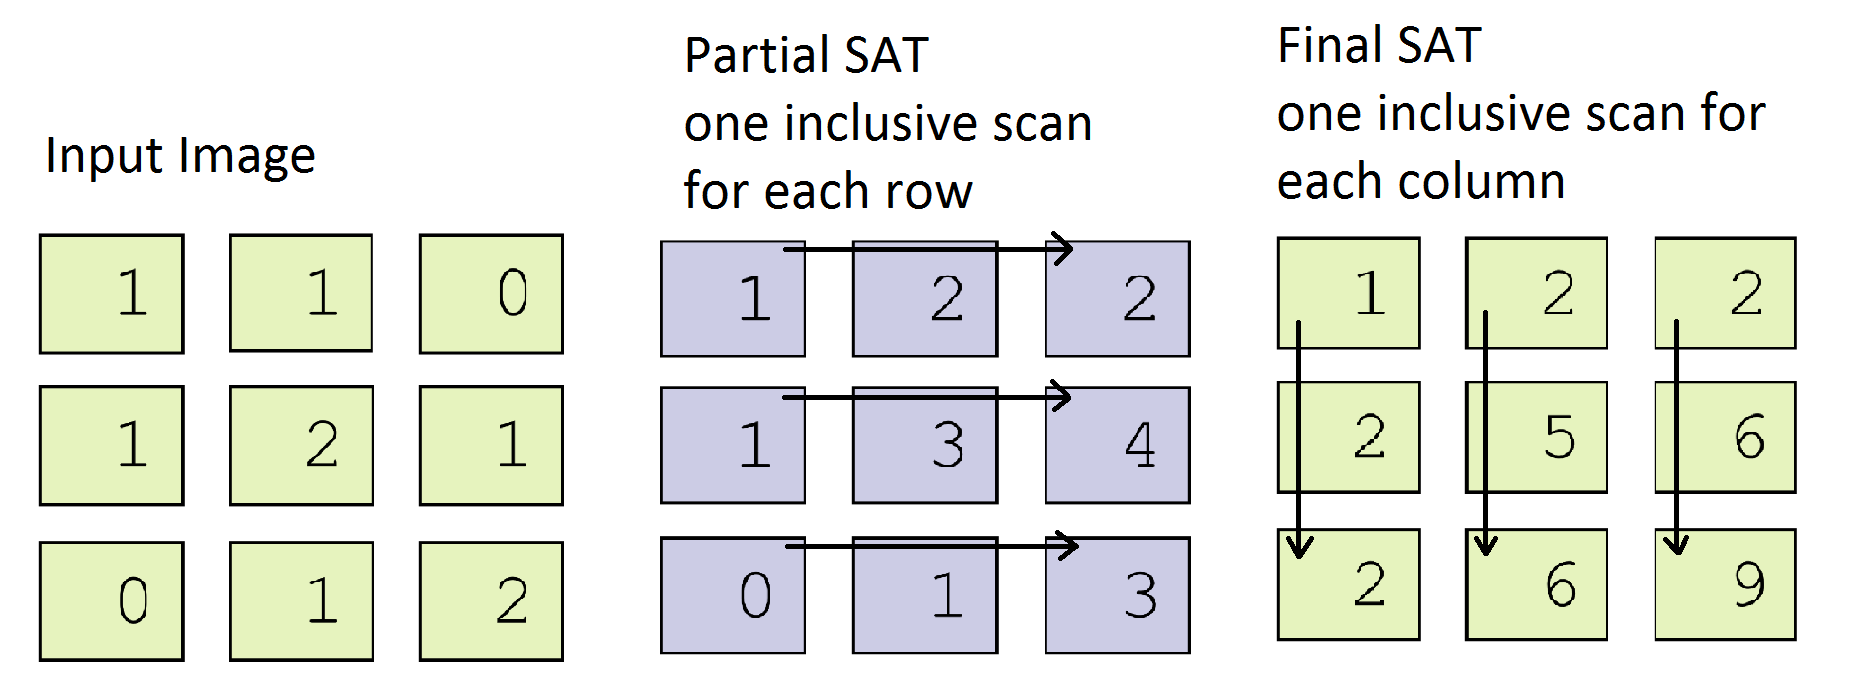
\includegraphics[width=\textwidth]{imm/iia/inclusive_scan}  
   	\caption{Scheme of the inclusive scan algorithm} 
   	\label{fig:inclusive_scan}
   \end{figure}
 
 \subsection{Balanced Trees Parallel Scan algorithm}
 For simplicity, i will explain the algorithm for a 1D-array.
 The goal is to evaluate the SAT of a single row which is also known as the prefix sum, also called cumulative sum, inclusive scan. \cite{sat1}
 
 A prefix sum can be calculated in parallel by the following steps.

 \begin{enumerate}
 \item Build a balanced binary tree on the input data and sweep it to and from the root. 
 \item Traverse down from leaves to root building partial sums at internal nodes in the tree. 
 \item Traverse back up the tree building the scan from the partial sums.
 \end{enumerate}
 
  
 Figure \ref{fig:Balanced_tree} shows the scheme for an array of dimension 16.
 For a matrix, we implement this algorithm for each row and then for each column.
 
 \begin{figure}[h!]
 	\centering
 	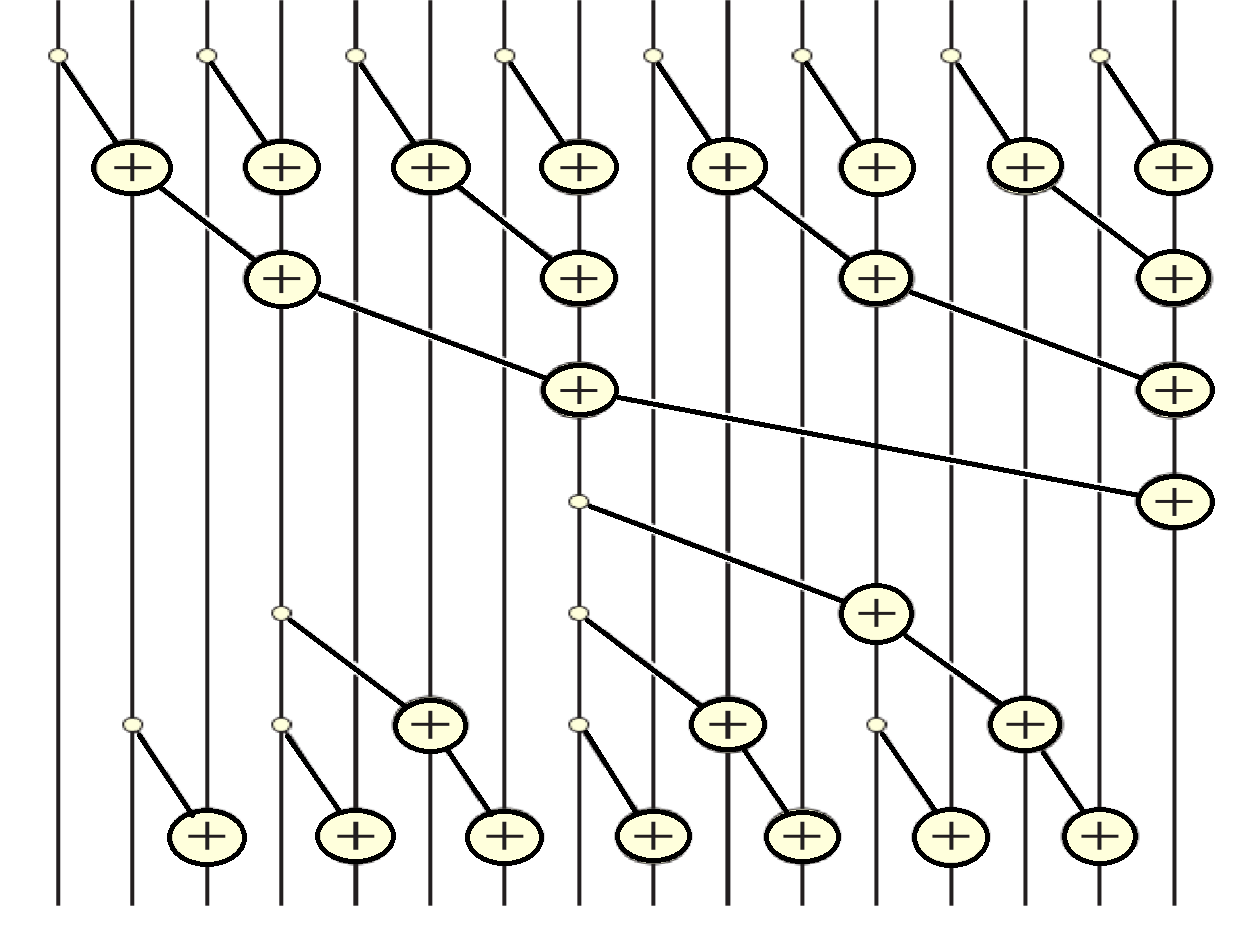
\includegraphics[width=\textwidth]{imm/iia/Balanced_tree0}  
 	\caption{Parallel Balnced Tree Algorithm for a 1D array} 
 	\label{fig:Balanced_tree}
 \end{figure}
 
\subsection{Comparing the 3 algorithm implementations}
Now that we know the implementation of these algorithm we can compare the area, i.e. the number of adders required, and the time between them.
In the table \ref{table:iia_tab} the unit time $ t $ is the time required to get the result of a single sum.


\begin{center}
	\begin{tabular}{ | p{1.7cm} | c | c | c | c |}
			
		\hline
		\label{table:iia_tab} & Inclusive scan & Balanced tree & This work & This work pipelined\\
		\hline
		Area & $ 2N(N-1) $ & $ 2N(2N-log_2 N -2) $ & $ N\cdotp N\cdotp log_2 N$ & $ N\cdotp N $\\
		\hline
		Time & $ 2(N-1) \cdotp t $
		& $ 2(2
		log_2 N-1)t $ &
		$ (log_2 N)2t $ & $ 2t $ \\
		\hline
		
	\end{tabular}
\end{center}
\subsection{Logic-In-Memory architecture} \label{sssec:1}
The \textit{Logic-In-Memory} is  a new architecture where logic and memory are embedded as unique entity instead of two separated ones (fig. \ref{fig:A}). \cite{lim}

The memory is made of small entities called \textit{bricks} populating two different layers: the bricks of each layer can communicate each other like in a matrix structure and only specifc bricks, called \textit{pillars}, are allowed to exchange data with the upper layer(fig. \ref{fig:B}). 
\begin{figure}[h!]
	\centering
	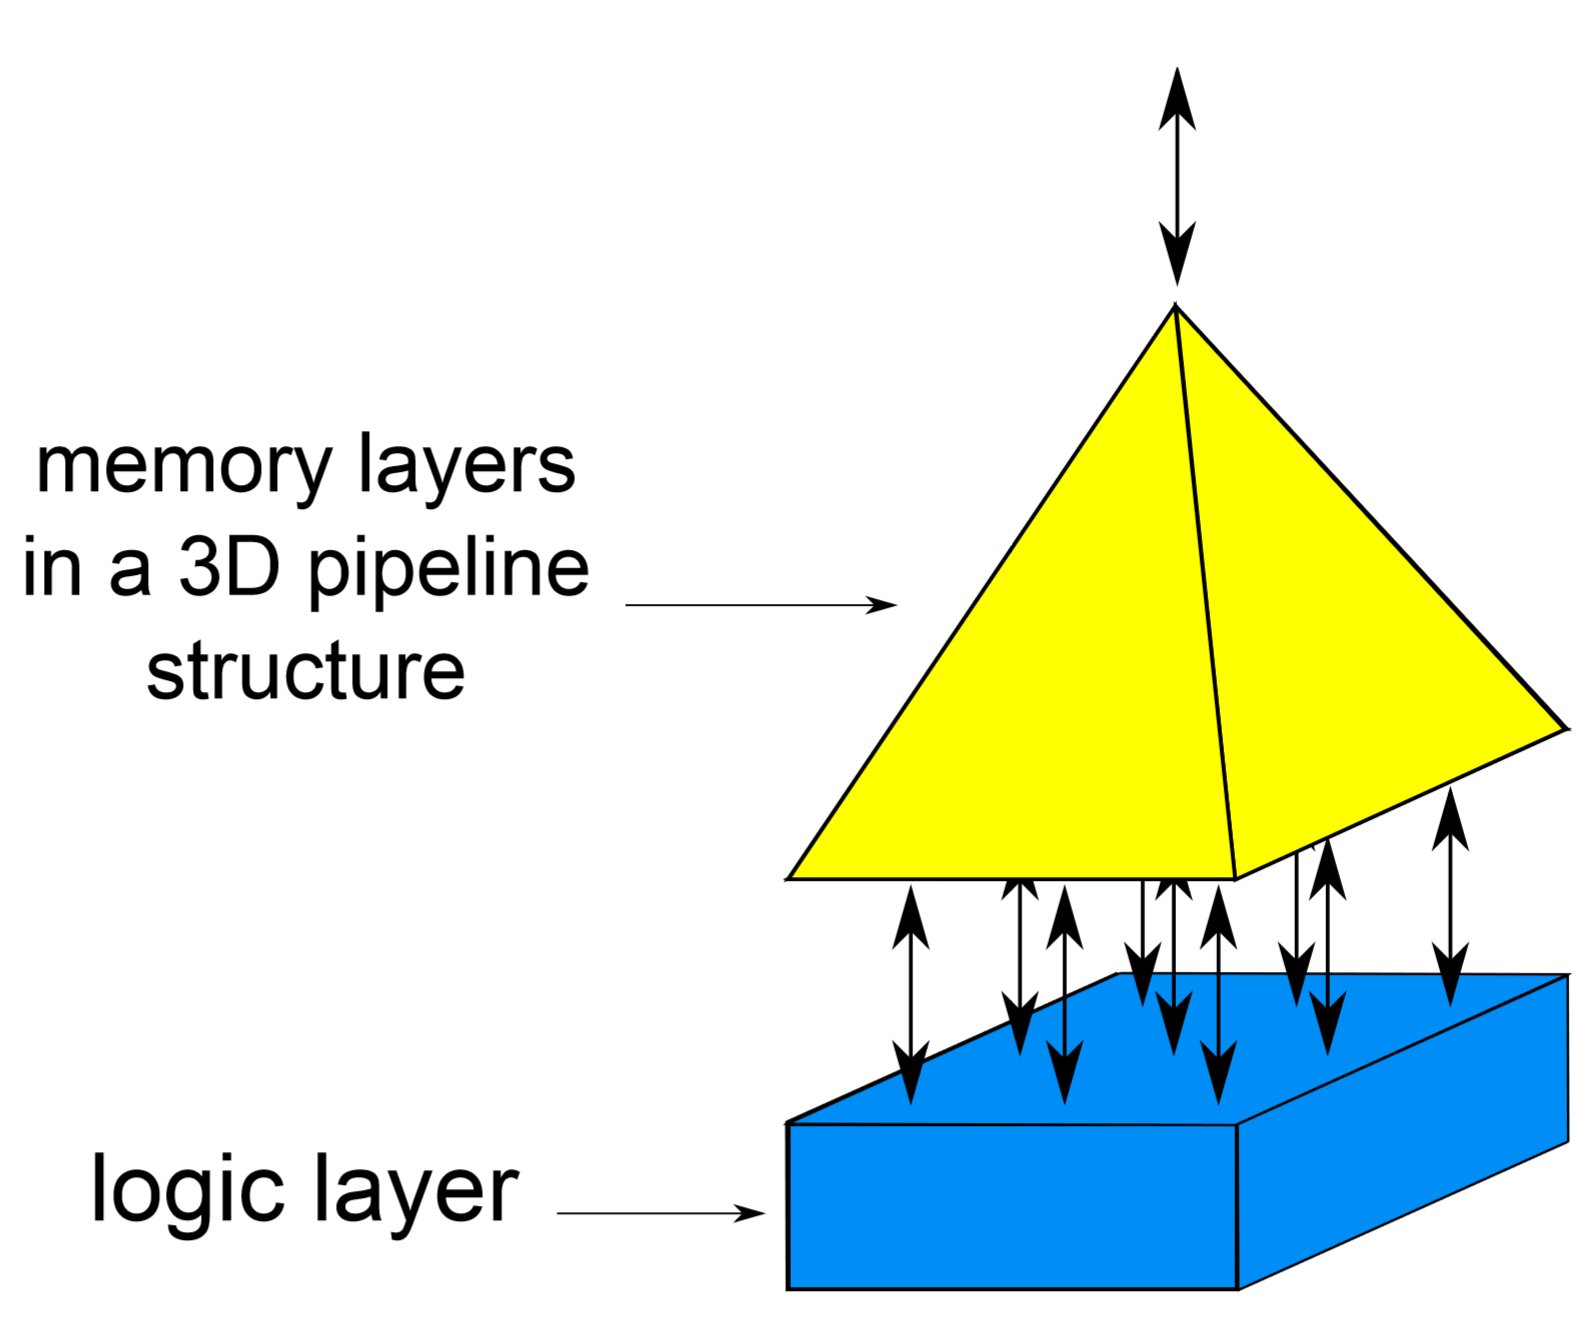
\includegraphics[width=\textwidth]{imm/iia/A.png}  
	\caption{Graphics representation of the architecture 2.0: the yellow pyramid represent the 3D pipeline of smart memories whereas the blue layer represent the programmable logic layer.} 
	\label{fig:A}
\end{figure}

\begin{figure}[h!]
	\centering
	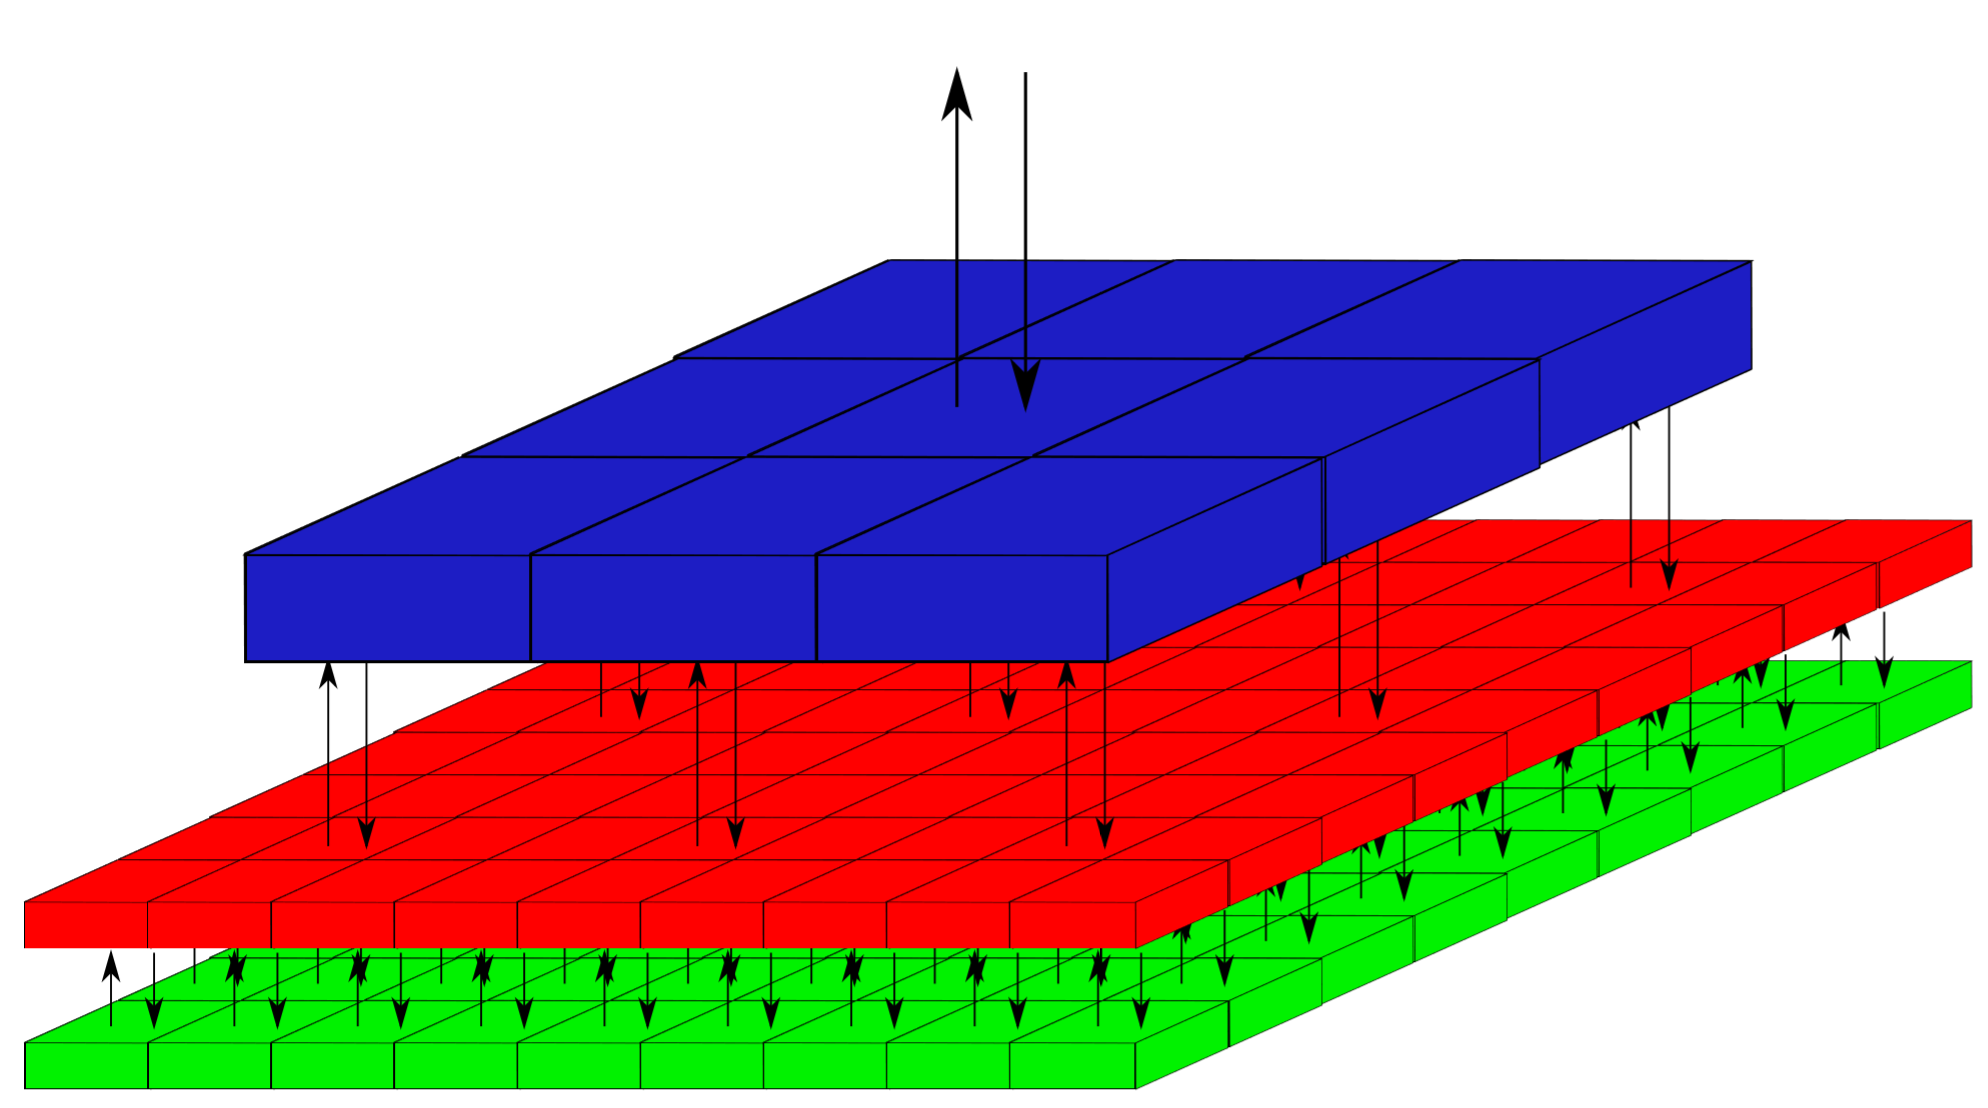
\includegraphics[width=\textwidth]{imm/iia/B.png}  
	\caption{ Structure of the LIM. The green layer represent the logic and is composed of 81 ALUs communicating each one with every brick of the bottom layer (red); the blue layer represent the upper plane and is composed of 9 bricks, one every 9 bricks of the bottom layer. Only the pillars of the bottom layer can communicate with the upper layer; only the pillar of the upper layer can exchange data with the outside.
	} 
	\label{fig:B}
\end{figure}
The upper layer is composed of a smaller number of bricks having a bigger memory capacity than the ones in the bottom layer: here the bricks are more in number but their memory capacitance is small. In addition, only this plane is able to communicate with the programmable logic layer: it is made of one ALU (arithmetic and logic unit) for each brick of the bottom layer. 
\clearpage
\subsection{Comparison with the LIM architecture}
I take the results of the LIM's architecture
 The pseudocode for the LIM architecture is the following:
 \begin{enumerate}
 	\item Each cell reads its own value;
 	\item Sums its value to the one received from the NORTH and sends the result to the SOUTH;
 	\item Samples the value coming from the WEST, sums it to the previous result and sends it to the EAST;
 	\item Writes the final result in its own memory;
\end{enumerate}
 The main advantage of the LIM architecture is the parallelism: the presence of many cells that can work autonomously greatly increases the speed of the computation of algorithms that can be executed in parallel.
  The duration of the algorithm depends on the number of cells of the grid: in particular, supposing to have a grid of $ N \cdot N  $ cells, the total duration is equal to:
  \begin{itemize}
  	\item N clock cycles to write the data; 
  	\item 6N clock cycles to compute the algorithm; 
  	\item 2N+1 clock cycles to read the data through a remote read.   	
  \end{itemize} 
  Therefore,
  \begin{center}
  	$ t = N +6N +2N +1=9N +1 $
  \end{center}
  
  	 \begin{center}
  	 	\begin{tabular}{ | p{1.7cm} | c | c | c |}
  	 		
  	 		\hline
  	 		\label{table:iia2_tab} & LIM & This work & This work pipelined\\
  	 		\hline
  	 		Area & $ N\cdotp N$ cells  &  $ N\cdotp N\cdotp log_2 N $ adders  & $ N\cdotp N $ adders\\
  	 		\hline
  	 		Time & $ 9N +1  $ cycles
  	 		&
  	 		Time for $ 2(log_2 N) $ adders &Time for $ 2 $ adders\\
  	 		
  	 		\hline
  	 		
  	 	\end{tabular}
  	 \end{center}
\section{Characteristics of the Integral Image Algorithm}
\vspace{10pt}
{\large \textbf{PROCESSING ELEMENTS}}\vspace{10pt}\\
\begin{tabular}{ p{0.2cm} p{14.5cm}}
	
&\textbf{1- Which kind of Processing element?}\\
&	Adder\vspace{7pt}\\
&	\textbf{2- Functionality}\\
&	Addition, summation\vspace{7pt}\\
&	\textbf{3- Complexity}\\
&	\begin{tabular}{ p{0.2cm} p{3cm} p{7cm}}
		
		&Not pipelined & Area $ N\cdot N\cdot log_2(N) $ adders\\
		& & Time$ (log_2N)2 $x(time for an addition) \vspace{3pt}\\
		& Pipelined & Area $ N^2 $ adders\\
		& & Time $ 2 $x(time for an addition)\\
		
	\end{tabular}\vspace{7pt}\\
&	\textbf{4- Parallelism}\\
&	All cells perform their Integral Image value in parallel.\vspace{7pt}\\
&	\textbf{5-Reconfigurability}\\
&	No\vspace{7pt}\\
&	\textbf{6- Programmability}\\
&	No\vspace{7pt}\\
&	\textbf{7- Need a dedicated memory?}\\
&	If the architecture is pipelined, you need to store the partial sum.\\
&	If not pipelined, no memory is required.\vspace{7pt}\\
	&\textbf{8- Relationship with I/O}\\
&	INPUT: values of the matrix's cells\\
&	OUTPUT: result of the integral image algorithm\end{tabular}\vspace{24pt}\\
\clearpage
{\large \textbf{\qquad }}\vspace{10pt}\\
{\large \textbf{MEMORY ELEMENTS}}\vspace{10pt}\\\begin{tabular}{ p{0.2cm} p{14.5cm}}
&\textbf{1- Need a clever memory LIM?}\\
&	No, but can be implemented\vspace{7pt}\\
&\textbf{2- Is there a data search algorithm?}\\
&	No\vspace{7pt}\\
&\textbf{	3-Interface mechanism with other PE or memories}\\
&	Communication required between cells (even between distant cells e.g. the center cell and the last cell).\vspace{7pt}\\
&	\textbf{4- Access mechanism}\\
&	(No memory for this implementation)\vspace{7pt}\\
&	\textbf{5- Hierarchization} \\
&	(No memory for this implementation)\vspace{7pt}\\
&\textbf{	6- Cache coherency} \\
&	(No memory for this implementation)\vspace{7pt}\\
&\textbf{	7- Is it a a transactional memory?}\\
&	(No memory for this implementation)\vspace{7pt}\\
&\textbf{	8- Are there virtualization (paging) mechanisms?}\\
&	(No memory for this implementation)\end{tabular}\vspace{14pt}\\
\vspace{10pt}\\
{\large\textbf{ENCODING INFORMATION}}\vspace{10pt}\\
\begin{tabular}{ p{0.2cm} p{14.5cm}}
	&\textbf{1-Which encoding is used?}\\
	&Binary encoding
\end{tabular}
\newpage
{\large\textbf{ }}\vspace{10pt}\\
{\large\textbf{CONNECTIONS}}\vspace{10pt}\\\begin{tabular}{ p{0.2cm} p{14.5cm}}
&\textbf{1-Packet Exchange Protocol}\\
&Directly\vspace{7pt}\\
&\textbf{2-Timing (asynchronou/synchronous)}\\
&Synchronous\vspace{7pt}\\
&\textbf{3-Are there multiple instances? }\\
&Yes, but the summation is not the same for all (some cells requires more data exchanging than others)\vspace{7pt}\\
&\textbf{4-Heterogeneity (Local/Distant I/O Connections)}\\
&Heterogeneous when storing the initial values to the cells, not heterogeneous when exchanging the data (sometimes you exchange data between local cells, the other times you exchange between distant cells.)\vspace{7pt}\\
&\textbf{5-Are there any buffers?}\\
&There are pipeline registers.
\end{tabular}\vspace{14pt}\\

%\chapter{Discrete cosine transform} \label{DCT}
A discrete cosine transform (DCT) expresses a finite sequence of data points in terms of a sum of cosine functions oscillating at different frequencies. DCTs are important to numerous applications in science and engineering, from lossy compression of audio (e.g. MP3) and images (e.g. JPEG). 
The DCT is often used in signal and image processing, especially for lossy compression, because it has a strong "energy compaction" property: in typical applications, most of the signal information tends to be concentrated in a few low-frequency components of the DCT. \cite{dct0}

There are different variations of the discrete cosine transform, but the most common one is the "DCT-II" which is also used in JPEG image compression and by MATLAB \circledR:



  \begin{equation} \label{eq:dct_eq}	
   X_{k}= \sum_{n=0}^{N-1} w(k)x_{n}cos\bigg[\frac{\pi}{N} (n+\frac{1}{2})k\bigg], \qquad k=0,1,...,N-1
 \end{equation}
 

    \[
    w(x)=\left\{
    \begin{array}{ll}
    \frac{1}{\sqrt{N}} & \qquad k=0\\
    &\\
    \sqrt{\frac{2}{N}} & \qquad 1\leqslant k \leqslant N-1\\
    \end{array}
    \right.
    \]
\bigskip
We can see the equation \ref{eq:dct_eq} as a product of matrices: we have to multiply the input vector $ x_{i} $  with a matrix of coefficients for cosine.
Thus the equation \ref{eq:dct_eq} can be rewritten as 

\begin{center}
\bigskip	
$\begin{bmatrix}X_{0}\\ X_{1} \\ \vdots \\X_{N-1} \end{bmatrix} = 
\begin{bmatrix}
	cos_{0,0} & cos_{0,1} & \cdots & cos_{0,n-1} \\
	cos_{1,0} & cos_{1,1} & \cdots & cos_{1,n-1} \\
	\vdots  & \vdots  & \ddots & \vdots  \\
	cos_{n-1,0} & cos_{n-1,1} & \cdots & cos_{n-1,n-1}  \\
\end{bmatrix} \begin{bmatrix}x_{0}\\ x_{1} \\ \vdots \\x_{N-1} \end{bmatrix}$

\end{center}
\bigskip
where the matrix of coefficients for cosine is the following

\begin{center}	
$ \begin{bmatrix} \frac{1}{\sqrt{N}}cos(\frac{\pi}{N}(0+\frac{1}{2})\cdotp 0) & \frac{1}{\sqrt{N}}cos(\frac{\pi}{N}(1+\frac{1}{2})\cdotp 0) & \cdots & \frac{1}{\sqrt{N}}cos(\frac{\pi}{N}(N-1+\frac{1}{2})\cdotp 0) \\
\sqrt{\frac{2}{N}}cos(\frac{\pi}{N}(0+\frac{1}{2})\cdotp 1) & \sqrt{\frac{2}{N}}cos(\frac{\pi}{N}(1+\frac{1}{2})\cdotp 1) & \cdots & \sqrt{\frac{2}{N}}cos(\frac{\pi}{N}(N-1+\frac{1}{2})\cdotp 1) \\
\vdots  & \vdots  & \ddots & \vdots  \\
\sqrt{\frac{2}{N}}cos(\frac{\pi}{N}(0+\frac{1}{2})\cdotp N-1) & \sqrt{\frac{2}{N}}cos(\frac{\pi}{N}(1+\frac{1}{2})\cdotp N-1) & \cdots & \sqrt{\frac{2}{N}}cos(\frac{\pi}{N}(N-1+\frac{1}{2})\cdotp N-1) \end{bmatrix} $
\bigskip
\end{center}

  \section{Hardware Implementation} \label{DCTH}
  \subsection{Not pipelined version}
  The result can be seen as a sum of products.
  Each element of the output array can be written as:
  \begin{center}
  	$ X_{i} =  x_{0}cos_{i,0}+x_{1}cos_{i,1}+ \cdots +x_{n-1}cos_{i,n-1}$
  \end{center}
  We can perform all the multiplications in parallel and then do an accumulator (or a chain of additions) with these product results. As we will see in the DCT synthesys result (\ref{synDCT}), there is no practical difference between the pipelined and not pipelined versions. The only difference is the area for the pipeline registers and the time for the addition chain over the multiplications (One addition is faster than one multiplications, however if the $ n $ number of additions in sequence to do is big enough, this time can offset the time for a single multiplication ).
  \begin{figure}[h!]
  	\centering	
  	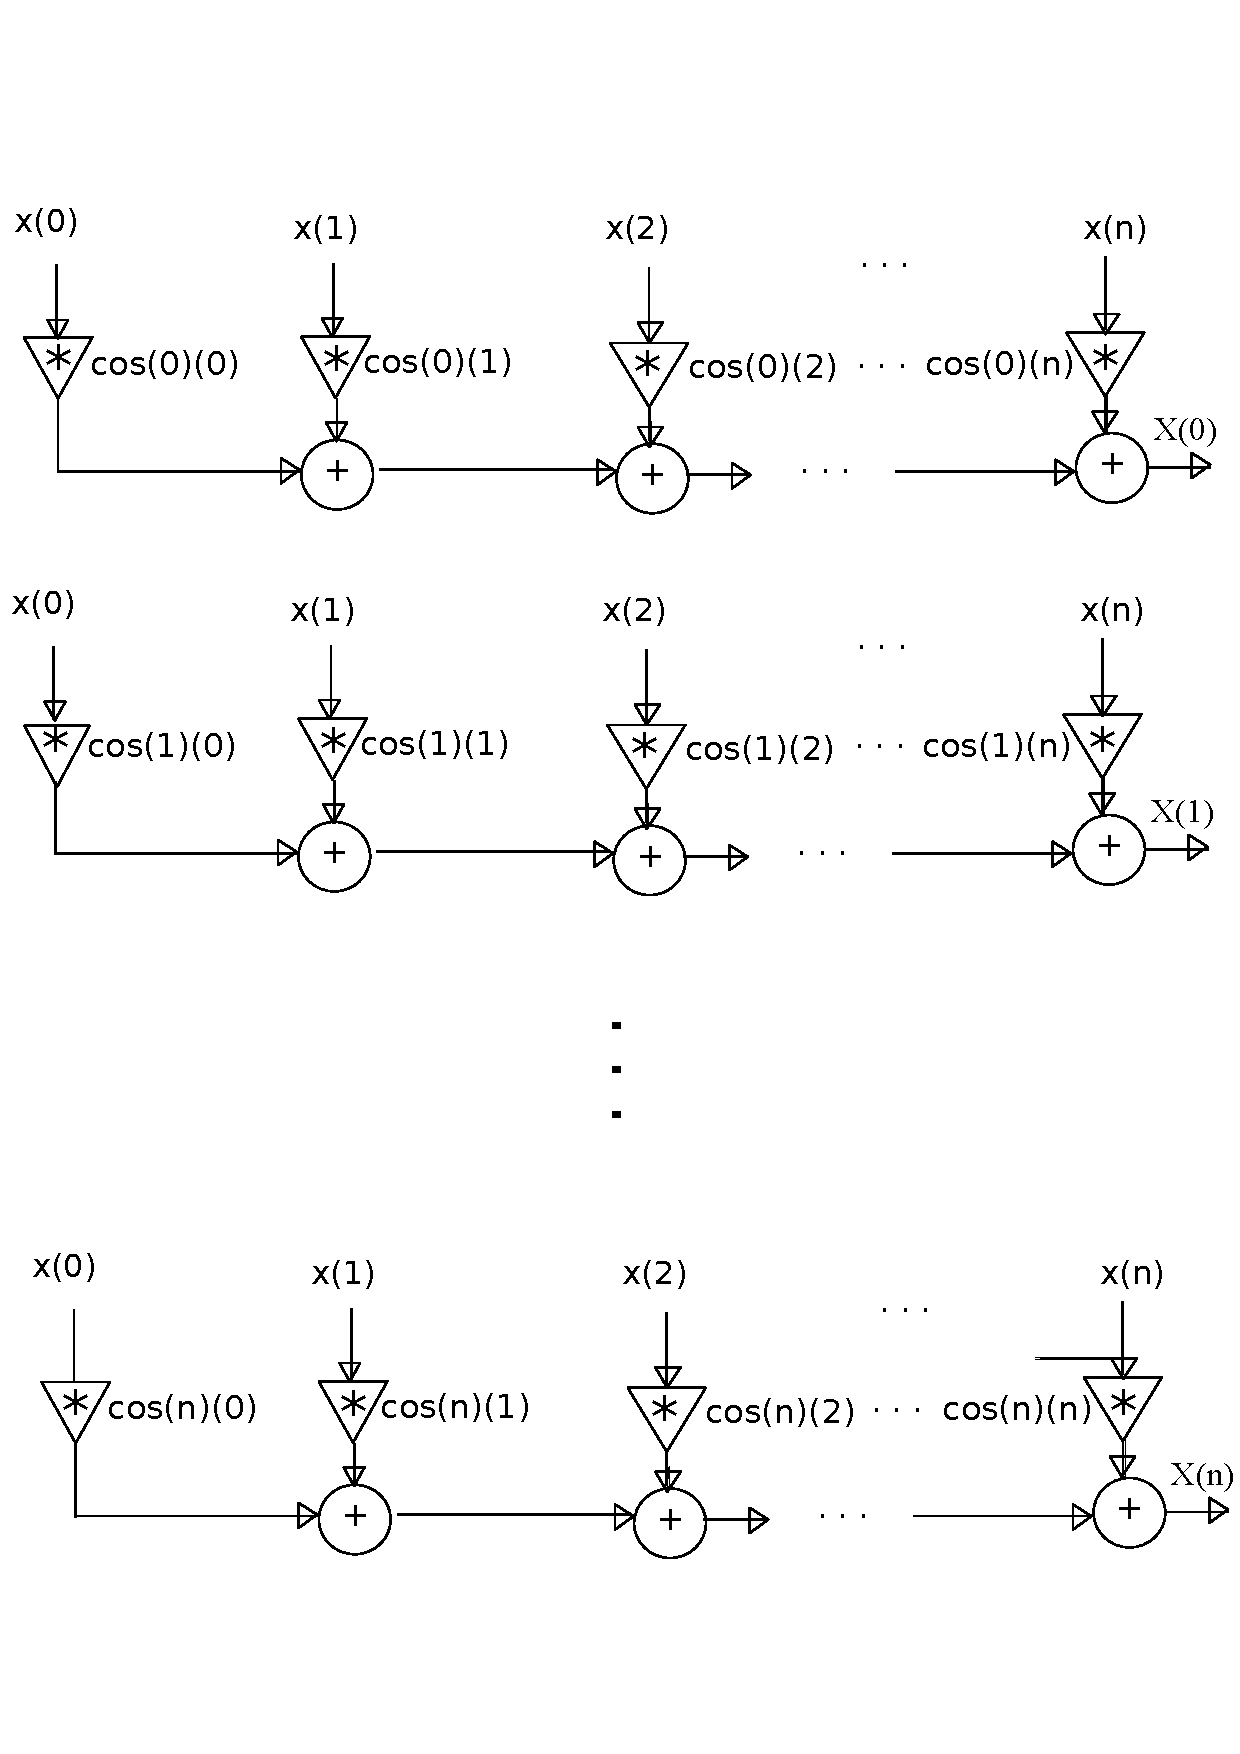
\includegraphics[width=0.9\textwidth]{imm/dct/dct_nopipe.pdf}  
  	\caption{Implementation of DCT algorithm (not pipelined). All multiplications are done in parallel} 
  	\label{fig:dct_nopipe}
  \end{figure}
  \clearpage
  \subsection{Pipelined version}
The result can be seen as a sum of products.
Each element of the output array can be written as:
\begin{center}
	$ X_{i} =  x_{0}cos_{i,0}+x_{1}cos_{i,1}+ \cdots +x_{n-1}cos_{i,n-1}$
\end{center}

Therefore, since there is no data dependencies between these elemnts, we can evaluate them in parallel.
\begin{enumerate}
\item In the first clock cycle we can perform the multiplication $ x_{0}cos_{i,0} $ for each element of the array.
\item In the second clock cycle we evaluate the second multiplication and sum it to the previous result $  [x_{0}cos_{i,0}] + x_{1}cos_{i,1} $
\item In the third clock cycle we evaluate the third multiplication and sum it to the previous result $  [x_{0}cos_{i,0} + x_{1}cos_{i,1}] + x_{2}cos_{i,2}$
\item We repeat this process until we reach the last term of this sum of product. In this clock cycle we have the final result $ X_{i} =  x_{0}cos_{i,0}+x_{1}cos_{i,1}+ \cdots +x_{n-1}cos_{i,n-1}  $

\end{enumerate}

In the following, we have the process explained in a matrix form, while figure \ref{fig:dct_scheme} represents this implementation in a Register to Transfer Level.


\begin{center}
	\bigskip	
	$\begin{bmatrix}X_{0}\\ X_{1} \\ \vdots \\X_{N-1} \end{bmatrix} = 
	\begin{bmatrix}
	
	\begin{matrix}
		x_{0}cos_{0,0}\\
		x_{0}cos_{1,0}\\
		\vdots\\
		\underbrace{x_{0}cos_{n-1,0}}_{1^{st} step}
		
		\end{matrix}
		
		\begin{matrix}
		\quad+\quad\\
		\quad+\quad\\
		\quad	\vdots\\
		\quad+\quad\\
		\\
		\end{matrix}
		
	\begin{matrix}
	x_{1}cos_{0,1}\\
	x_{1}cos_{1,1}\\
	\vdots\\
	\underbrace{x_{1}cos_{n-1,1}}_{2^{nd} step}
	
	\end{matrix}
	
		\begin{matrix}
		\quad+\quad\\
		\quad+\quad\\
		\quad\vdots\\
		\quad+\quad\\
		\\
		\end{matrix}
	
	\begin{matrix}
	\quad\cdots\\
	\quad\cdots\\
	\quad\vdots\\
	\quad\cdots\\
	\\
	\end{matrix}
	
		\begin{matrix}
		\quad+\quad\\
		\quad+\quad\\
		\quad\vdots\\
		\quad+\quad\\
		\\
		\end{matrix}
		
		\begin{matrix}
		x_{n-1}cos_{0,n-1}\\
		x_{n-1}cos_{1,n-1}\\
		\vdots\\
		\underbrace{x_{n-1}cos_{n-1,n-1}}_{last \quad step}
		
		\end{matrix}

	\end{bmatrix} $
	
\end{center}
\bigskip
\begin{figure}[h!]
	\centering	
	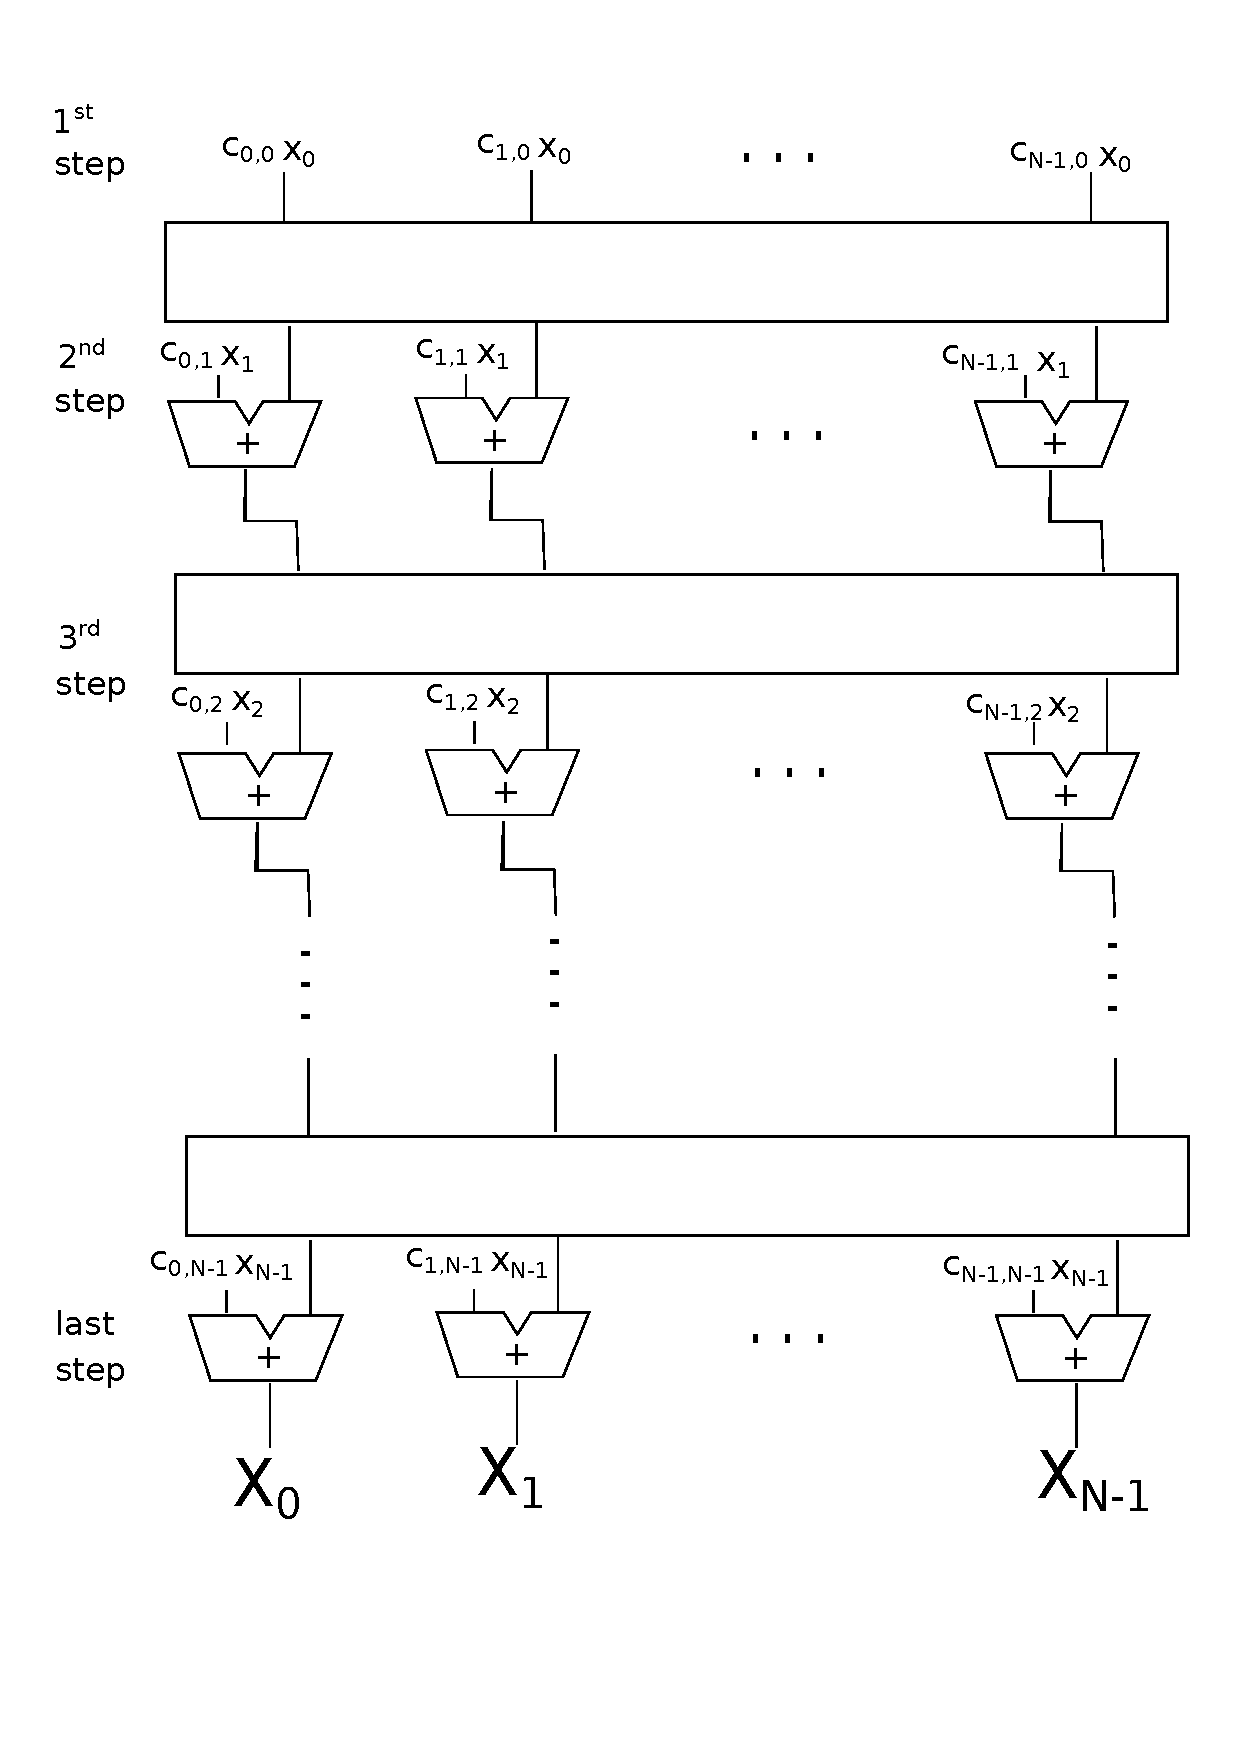
\includegraphics[width=0.9\textwidth]{imm/dct/dct_scheme.pdf}  
	\caption{Implementation of DCT algorithm (pipelined)} 
	\label{fig:dct_scheme}
\end{figure}
\clearpage
\section{Simulation and Test} 
I performed some tests of this implementation with different size and dimension. In the fig.\ref{fig:tb_dct} we can see the results of an array of six elements.

\begin{figure}[h!]
	\centering	
	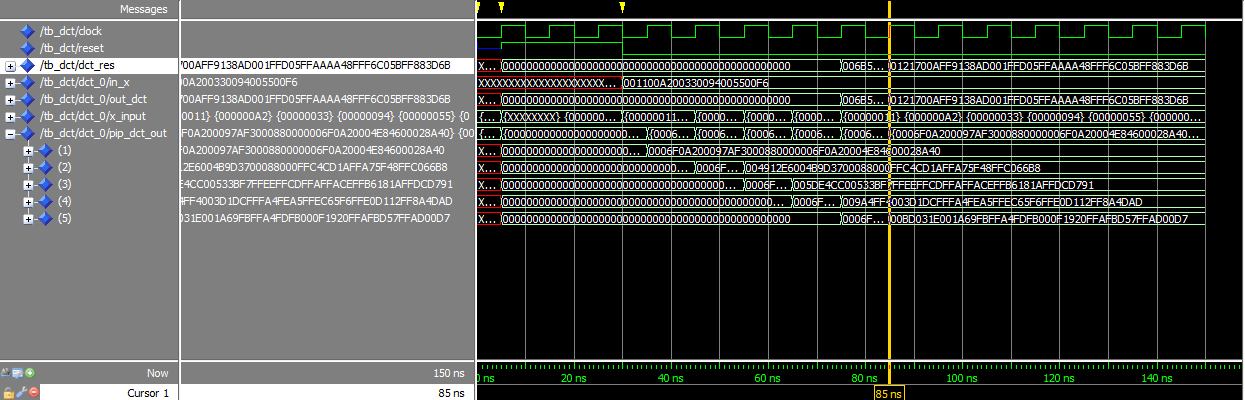
\includegraphics[width=\textwidth]{imm/dct/wave1.png}  
	\caption{Discrete cosine transform-Results of the simulation} 
	\label{fig:tb_dct}
\end{figure}
The simulation shows the input array:
\begin{center}
	$ in\_x=0x001100A200330094005500F6$ 
\end{center}
that stands for 
\begin{center}
	$ x_{0}=0x0011$\\
$ 	x_{1}=0x00A2 $\\
	$ x_{2}=0x0033 $ \\
	$ x_{3}=0x0094 $ \\
	$ x_{4}=0x0055 $ \\
	$x_{5}=0x00F6$
\end{center} which in decimal is
\begin{center}

$ x_{0}=17$ \\$ x_{1}=162 $\\$ x_{2}=51 $\\$ x_{3}=148 $\\$ x_{4}=85 $\\$x_{5}=246$
\end{center}
During the first 6 clock cycles, we can see the partial sum and multiplications.
The output is available in the $ 6^{th} $ clock cycle after the reset:\begin{center}
	 $ dct\_res=0x0121700AFF9138AD001FFD05FFAAAA48FFF6C05BFF883D6B $
\end{center} that stands for\begin{center}
 $ X_{0}=0x0121700A$ \\$X_{1}=0xFF9138AD$\\$X_{2}=0x001FFD05$\\$X_{3}=0xFFAAAA48
 $\\$X_{4}=0xFFF6C05B$\\$X_{5}=0xFF883D6B $
\end{center} and if we convert them in decimal by reserving 16 bits for the floating points, we get 
\begin{center}
	 $ X_{0}=289.437653$\\$X_{1}=-110.778610$\\$X_{2}=31.988358$\\$X_{3}=-85.334839$
	 \\$X_{4}=-9.248611$\\$X_{5}=-119.760086 $
\end{center}
 We checked this result by using the function $ dct $ on Matlab (Figure \ref{fig:dct_res_mat}).
We see that it differs from the Matlab result by a value in the order of 1/100. This depends on the precision used for the implementation, especially when converting the cosine values into binary.
 




\begin{figure}[h!]
	\centering	
	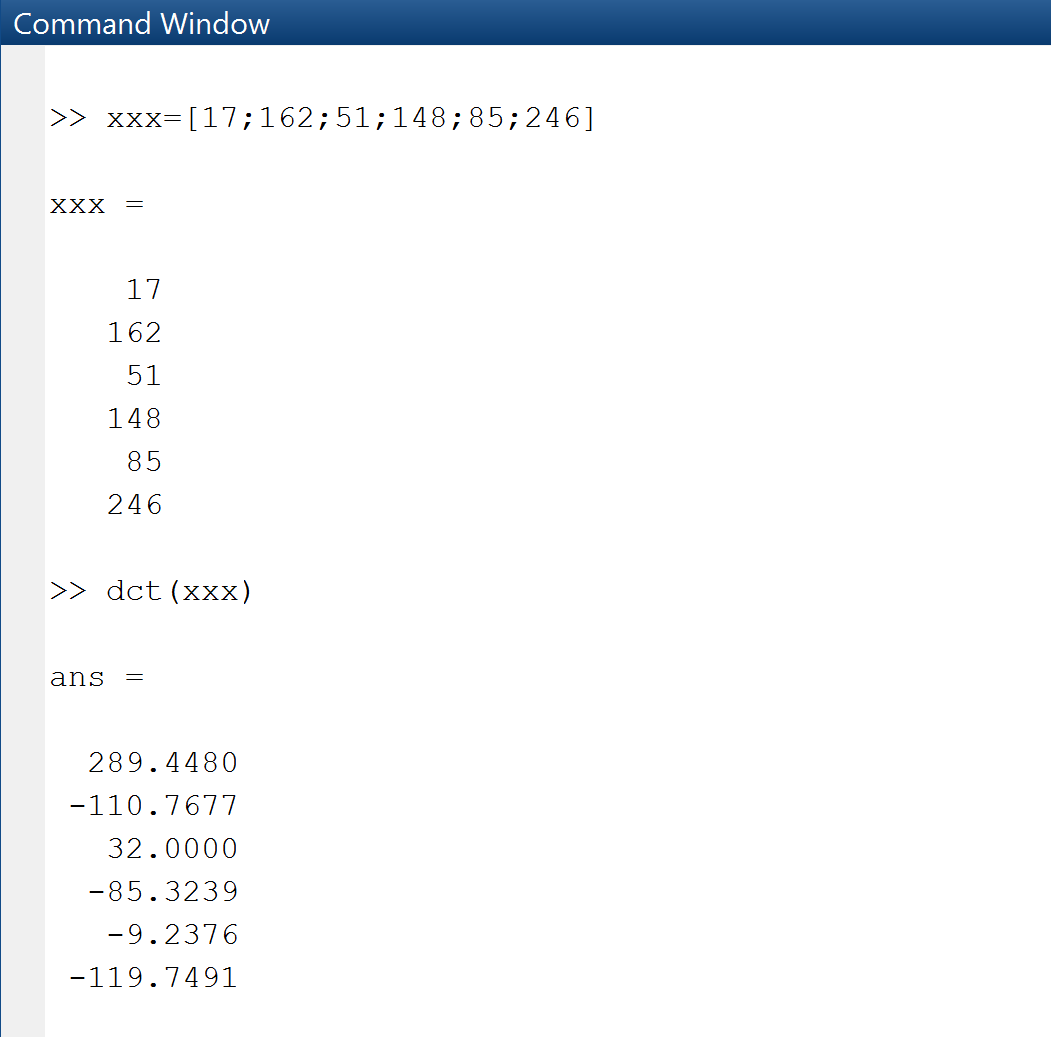
\includegraphics[width=0.9\textwidth]{imm/dct/dct_res_matlab.png}  
	\caption{DCT result in MATLAB} 
	\label{fig:dct_res_mat}
\end{figure}

\clearpage
\section{Comparison}
 \subsection{Systolic array architecture}
A systolic array can be seen as a homogeneous network of funtional units (called also \textbf{nodes} or \textit{Data Processing Units (DPU)}) which elaborate data and exchange them with their neighbours following a flow; in particular each FU receives the data from its upstream FU, elaborates it and passes it downstream. 
Each FU is indipendent from the others and executes only one operation over a huge amount of data; for this reason, systolic arrays are classified as SIMD (single instruction, multiple data) architectures. 
The particular name ("systolic") derives from the fact that inside the array there is a continuous flow of data propagating from a FU to the next one resembling the flow of the blood in the human body.
Usually, systolic arrays cannot be programmed and for this reason the circuit has to be designed $ ad-hoc $. This kind of structure is made of simple FUs which usually implement a simple operation (addition, multiplication, ecc..) and that have a very small memory capability. The main purpose of each node is to compute a data and send it to the next FU following the flow. \cite{dct2}

\begin{figure}[h!]
	\centering	
	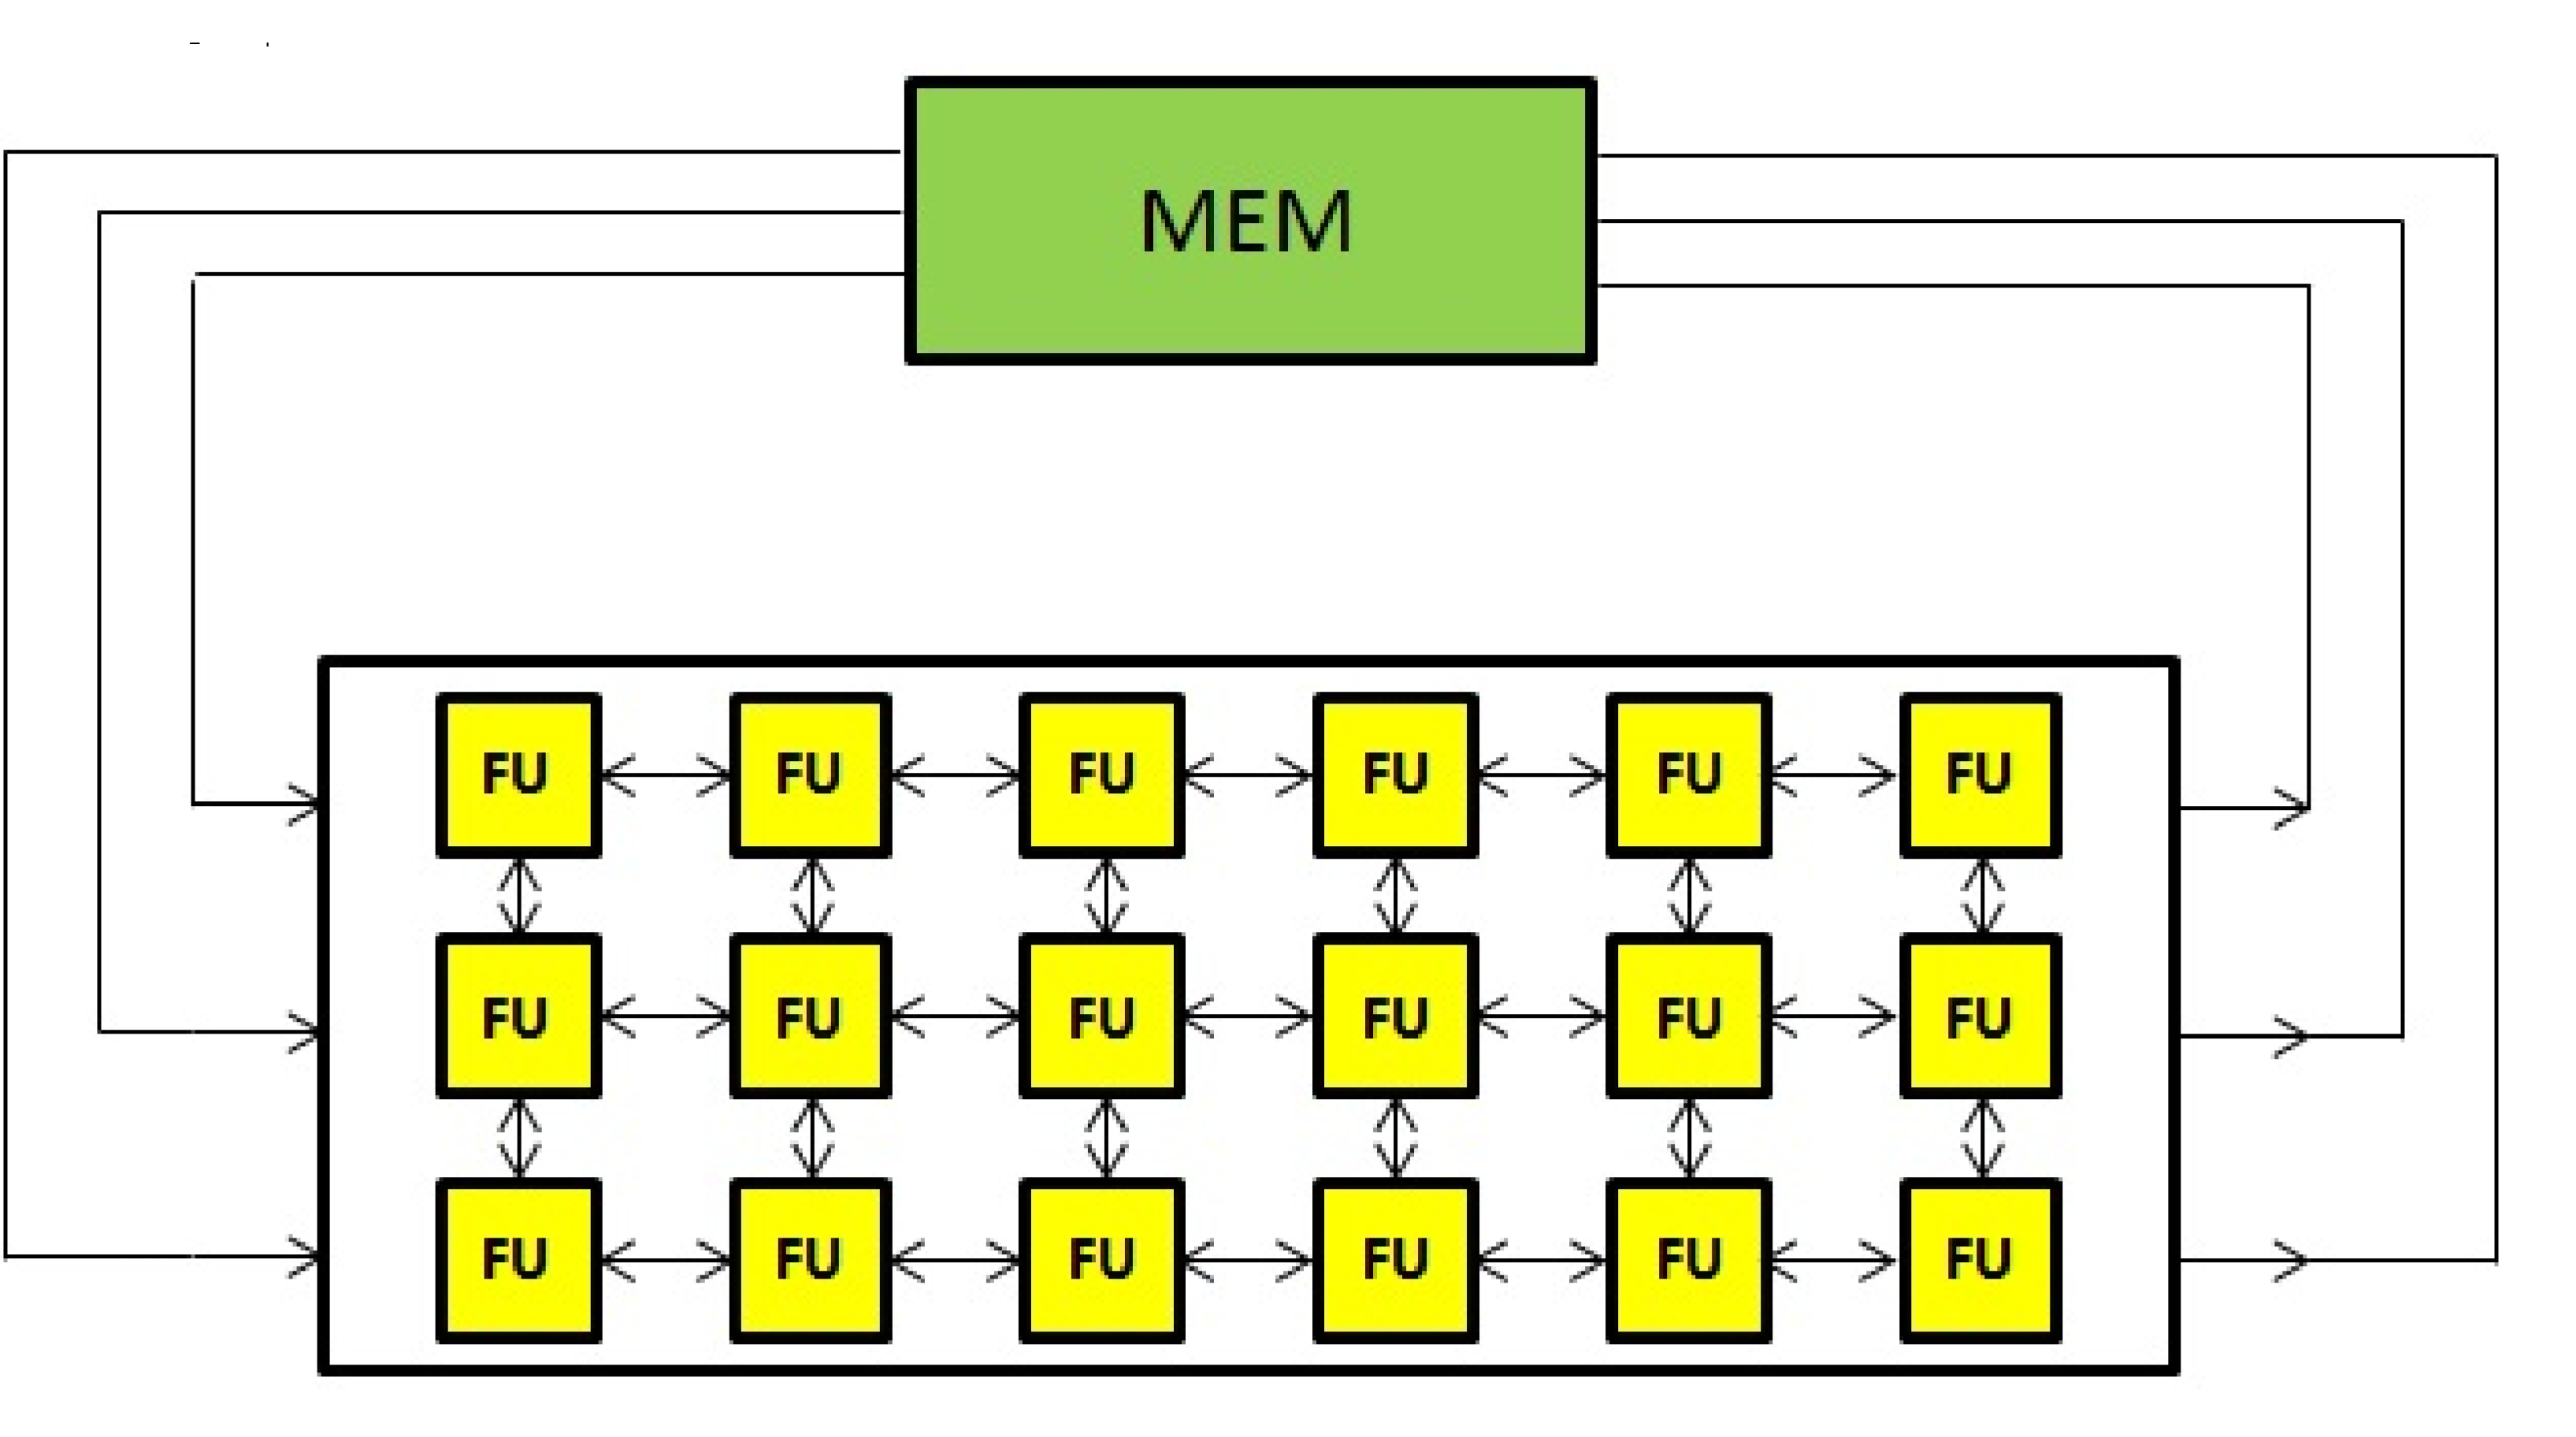
\includegraphics[width=0.9\textwidth]{imm/dct/dct_sa0.png}  
	\caption{ A generic figure of a systolic array; it is possible to notice the presence of parallel inputs and parallel outputs. Data are taken from the memory, eleborated along the multiple paths of FUs and then stored again in the memory.
		} 
	\label{fig:dct_sa0}
\end{figure}
\clearpage
 \subsection{Comparison with systolic array implementation}  \label{DCTSA}
 The DCT has been implemented in a systolic array architecture \cite{dct2} with the following structure (Fig \ref{fig:dct_sa1})
 
 \begin{figure}[h!]
 	\centering
 	 	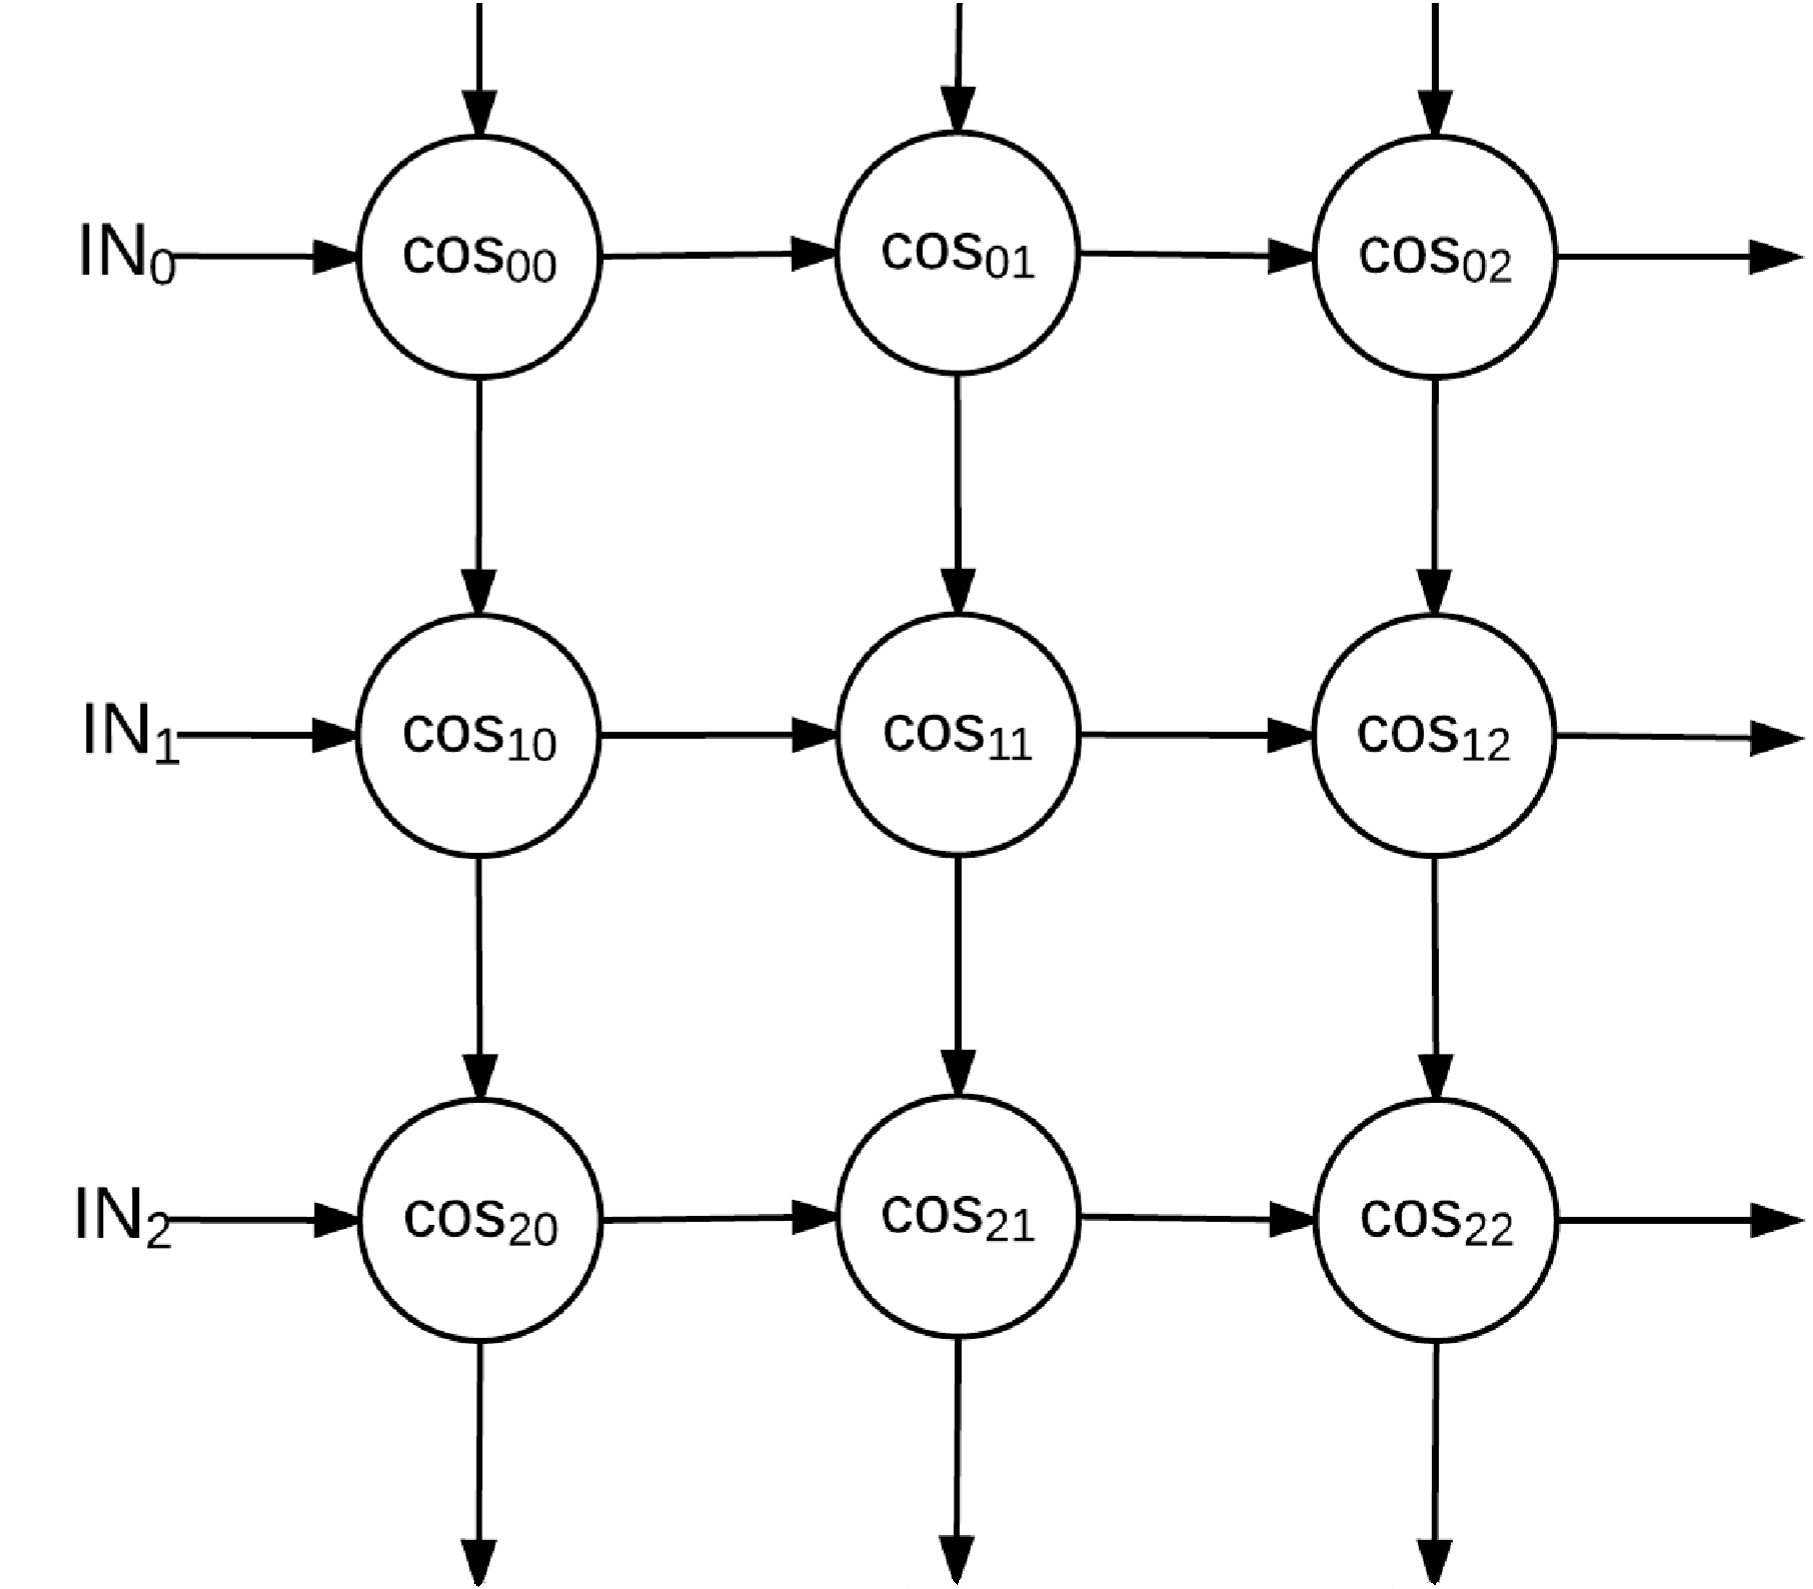
\includegraphics[width=0.75\textwidth]{imm/dct/dct_sa1.png}  
 	% 	\resizebox{[width=\textwidth]}{!}{\input{imm/dct/dct_scheme.pdf_tex}}
 	\caption{Implementation of DCT algorithm in a systolic array architecture} 
 	\label{fig:dct_sa1}
 \end{figure}
 
 Given an input array (from the left), each element of this array will be multiplied by the values of the cosine matrix, previously stored in the internal register (Fig \ref{fig:dct_sa2}).
 At the output of each processing element (Fig \ref{fig:dct_sa2}), we have tha product $ IN_{i}\cdot cos_{i,j} $ towards the bottom and the $ IN_{i} $ value toward the right.
 
  \begin{figure}[h!]
  	\centering
  	  	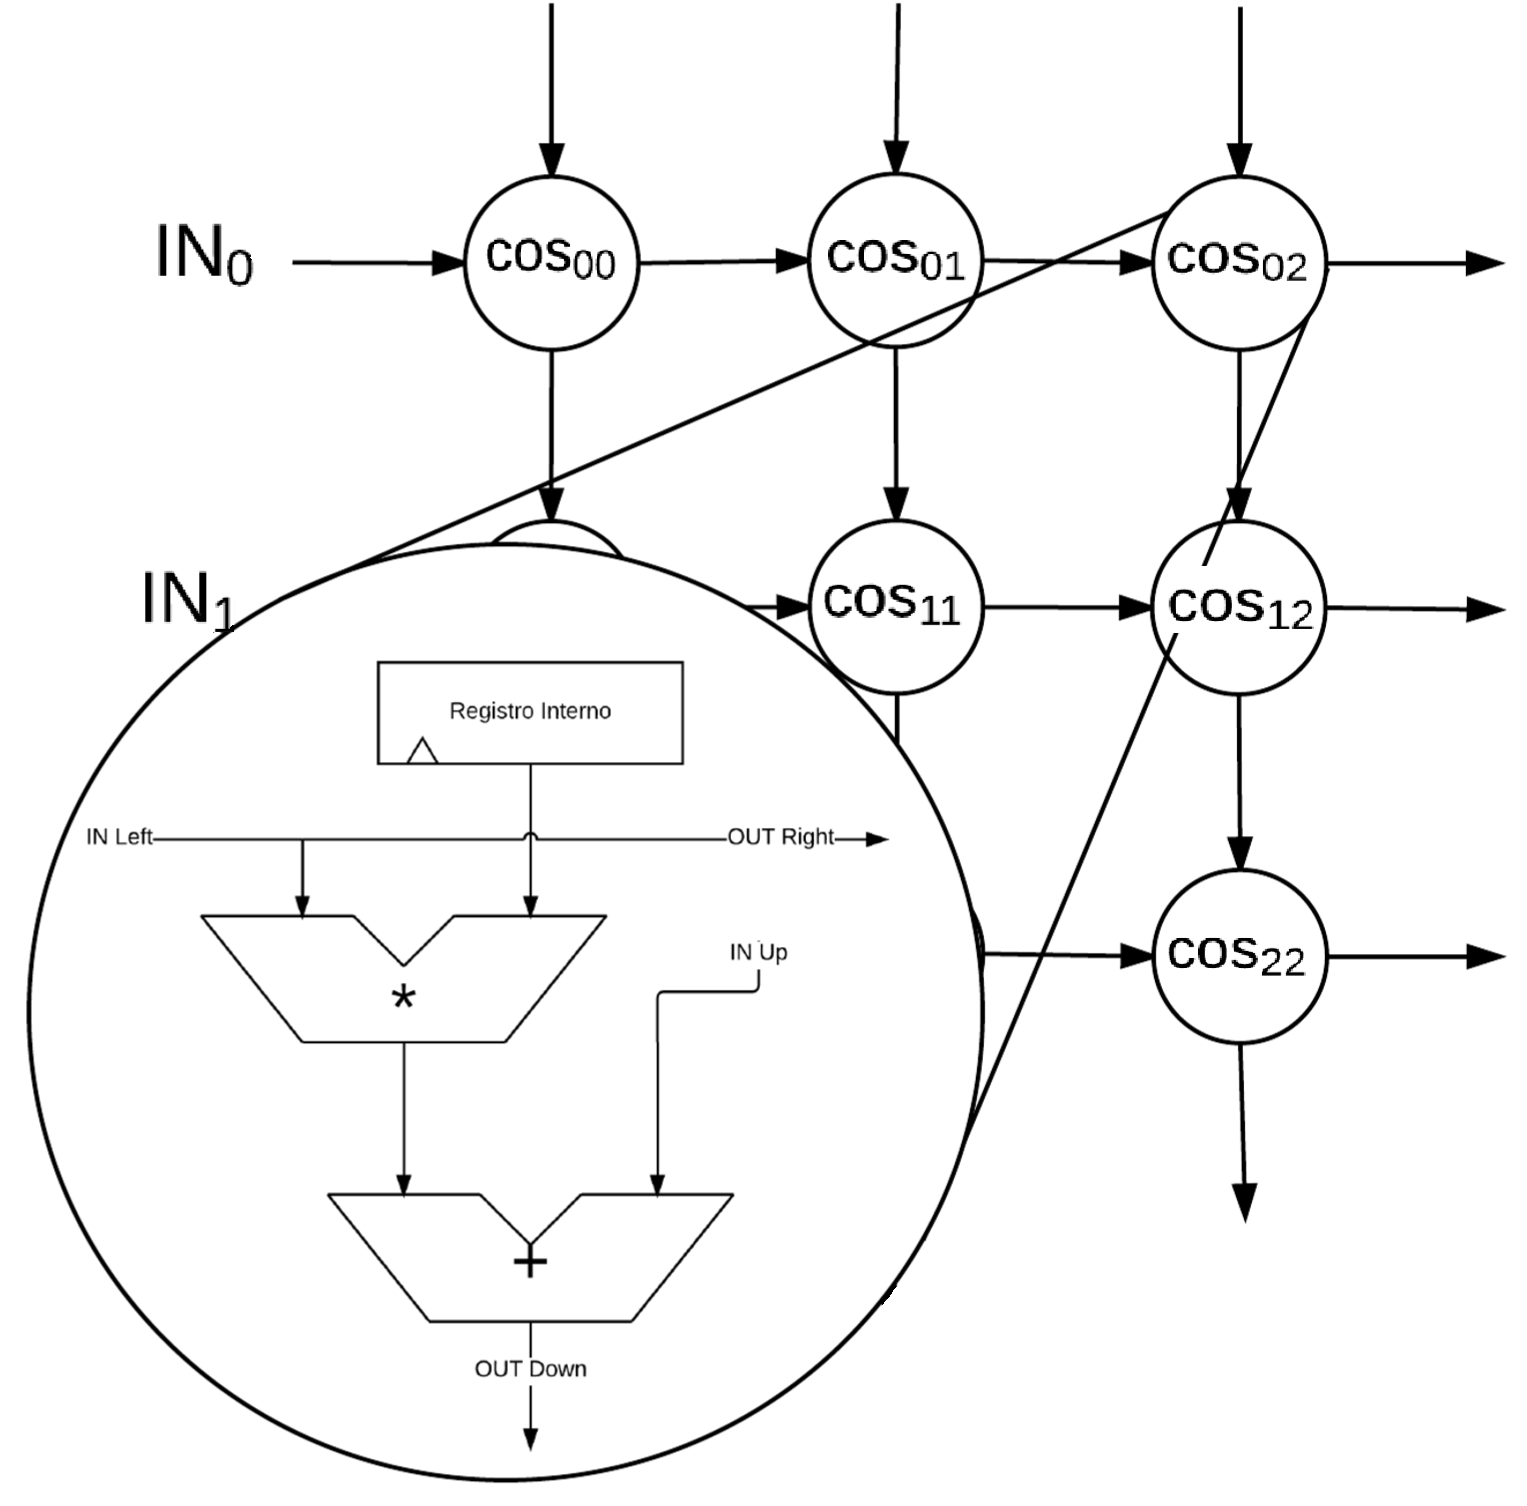
\includegraphics[width=0.75\textwidth]{imm/dct/dct_sa2.png}  
  	% 	\resizebox{[width=\textwidth]}{!}{\input{imm/dct/dct_scheme.pdf_tex}}
  	\caption{Processing element structure} 
  	\label{fig:dct_sa2}
  \end{figure}
   
  The simulation's results of this implementation are shown in figure \ref{fig:dct_sa3} with a check of the result in MATLAB (Fig. \ref{fig:dct_sa4})
  As we can see from the simulation, for an array of size $ N $, we need $ 2N-1 $ clock cycles to get the result.
  On the other hand, by looking to the structure of the systolic array, we can deduct the area to be $ N \cdot N $ processing elements.\\
  An important observation has to be done for the table \ref{table:dct_tab}.
  For the implementation not pipelined described in \ref{DCTH}, the critical path is made of one multiplier and a cascade of $ N-1 $ adders, this is due because all the multiplication can be done in parallel, while the adders have some dependencies between them.
   \begin{center}
   	\begin{tabular}{ | p{1.3cm} | >{\centering\arraybackslash}p{4cm} | >{\centering\arraybackslash}p{4cm} | >{\centering\arraybackslash}p{4cm} |}
   		\hline
   		\label{table:dct_tab} & Systolic array & This work & This work pipelined\\
   		\hline
   		Area & $ N^{2}$ $ moltiplications $ \qquad \qquad$N^{2}$ $ additions $  & $N^{2}
   $ $moltiplications$ \qquad \qquad $ N^{2} $ $additions$ & $ N$ $ moltiplications$ \qquad \qquad $ N$ $ additions$\\
   		\hline
   		Time & $ (2N-1) $ x (time for an addition and a multiplication)&
   		
   		$ (N-1) $x(time for an addition) + time for a single multiplication & time for an addition and a multiplication. Also the synthesy's results \ref{synDCT} are concordant with this theory.
   		 \\
   		\hline
   		
   	\end{tabular}
   \end{center}
        \begin{figure}[h!]
        	\centering
        	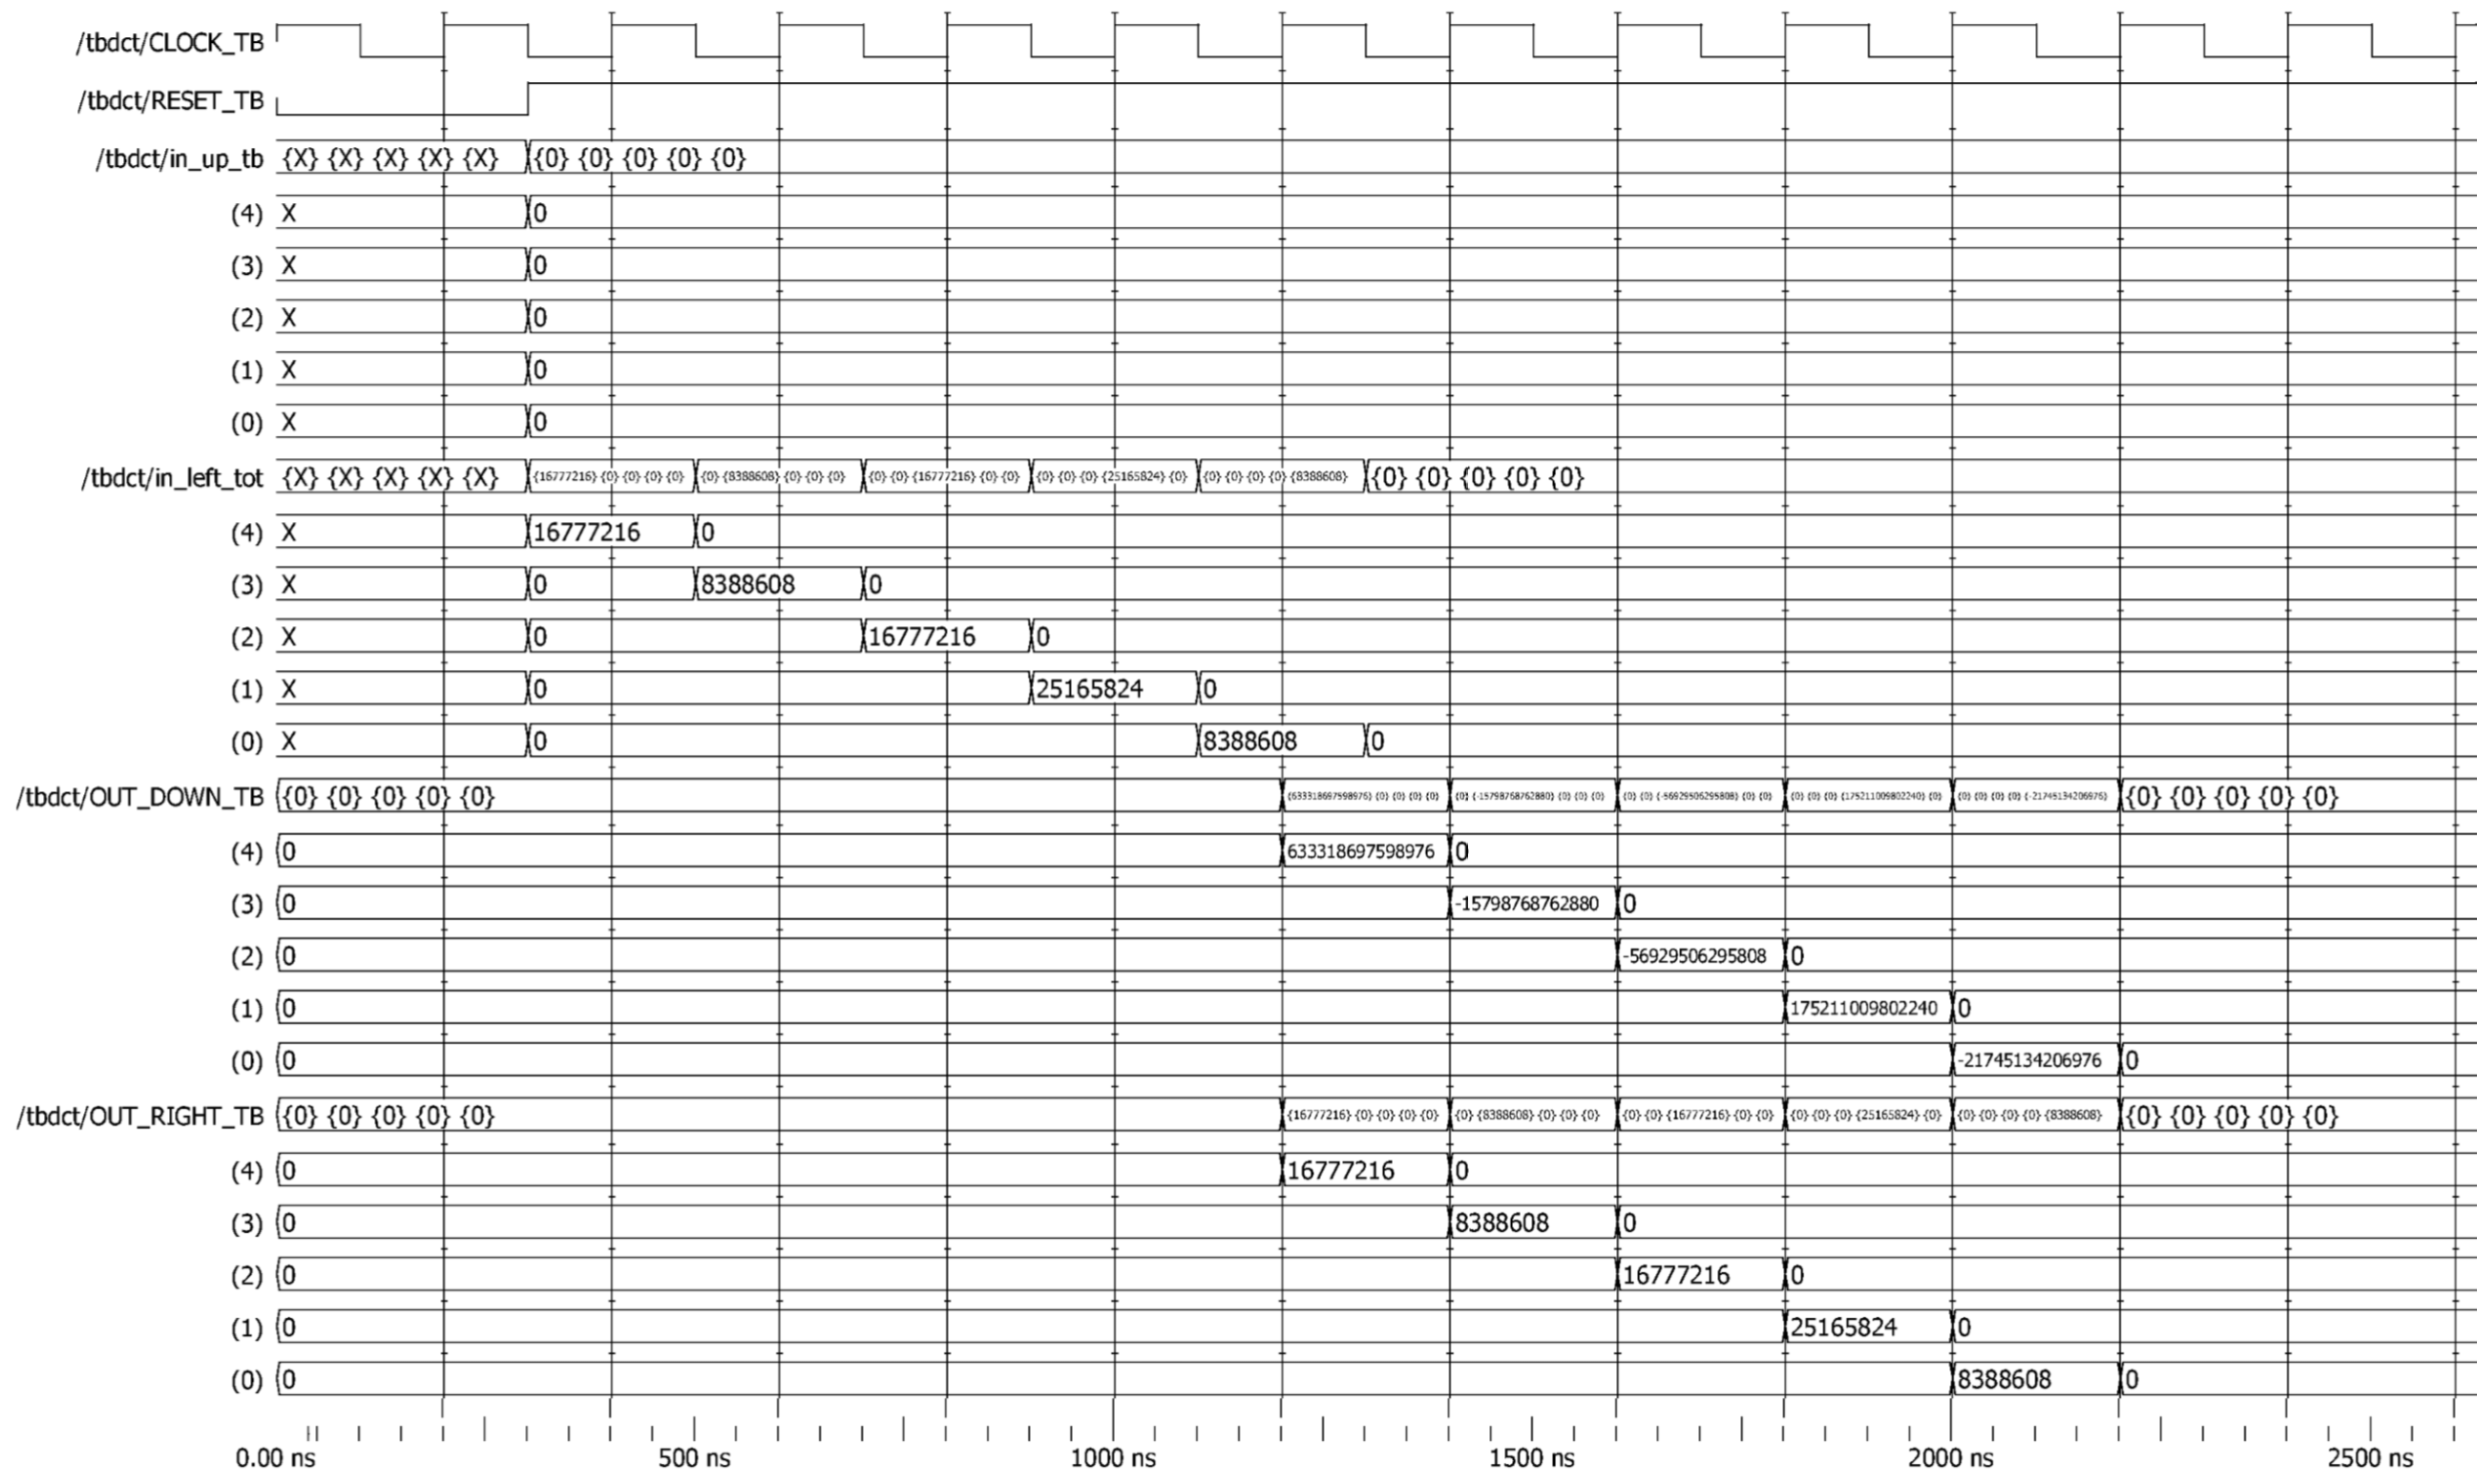
\includegraphics[width=\textwidth]{imm/dct/dct_sa3.png}  
        	\caption{Results of the DCT in a systolic array architecture} 
        	\label{fig:dct_sa3}
        \end{figure}
        
        \begin{figure}[h!]
        	\centering
        	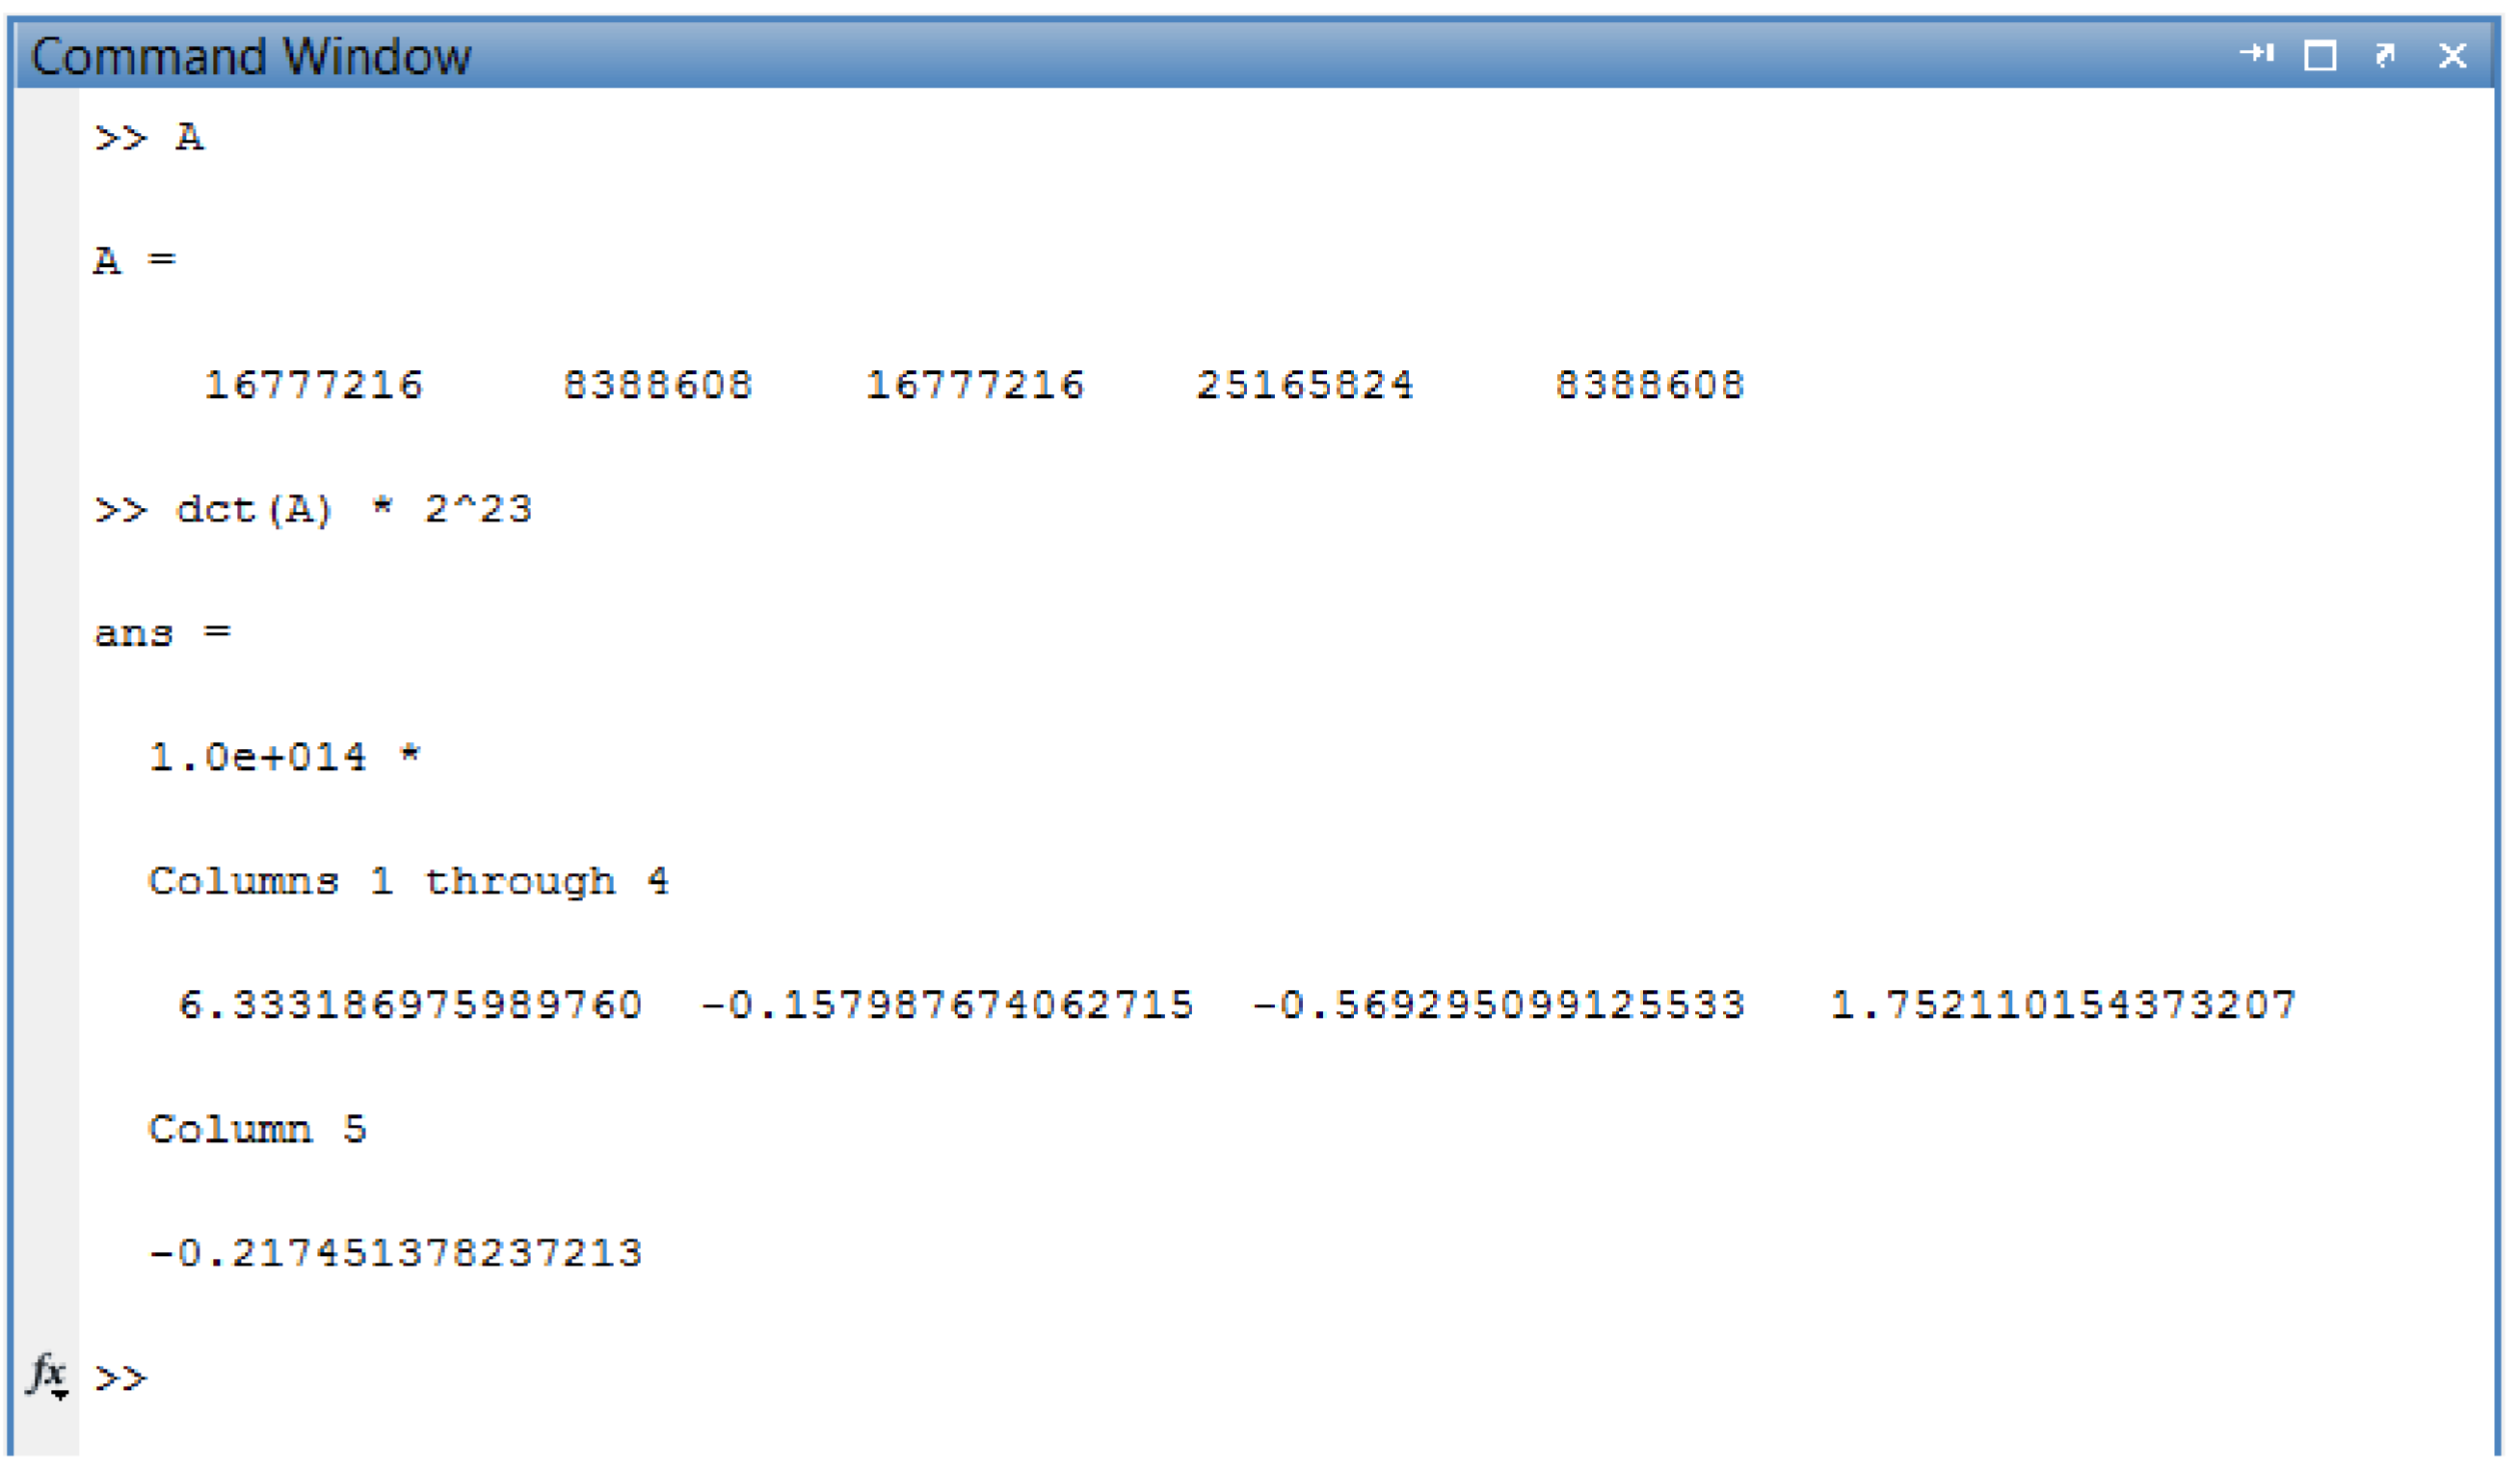
\includegraphics[width=\textwidth]{imm/dct/dct_sa4.png}  
        	\caption{Check results in MATLAB for systolic array architecture} 
        	\label{fig:dct_sa4}
        \end{figure}
   \clearpage
   
   
   \section{Characteristics of DCT}
   \vspace{10pt}
   {\large \textbf{PROCESSING ELEMENTS}}\vspace{10pt}\\
   \begin{tabular}{ p{0.2cm} p{14.5cm}}
   	
   	&\textbf{1- Which kind of Processing element?}\\
   	&	Adder, multiplier\vspace{7pt}\\
   	&	\textbf{2- Functionality}\\
   	&	Addition, mulltiplication, summation\vspace{7pt}\\
   	&	\textbf{3- Complexity}\\
   	&	\begin{tabular}{ p{0.2cm} p{2.5cm} p{10cm}}
   		
   		&Not pipelined & Area:\qquad $ N^2 $ multiplier, $ N^2 $ additions\\
   		& & Time: \qquad8x(time for a multiplier followed by an adder) \vspace{3pt}\\
   		& Pipelined & Area: \qquad $ N$ multiplier, $ N$ additions\\
   		& & Time: \qquad time for a multiplication followed by an adder\\
   		
   	\end{tabular}\vspace{7pt}\\
   	&	\textbf{4- Parallelism}\\
   	&	Multiplications and summation are done in parallel.\vspace{7pt}\\
   	&	\textbf{5-Reconfigurability}\\
   	&	No\vspace{7pt}\\
   	&	\textbf{6- Programmability}\\
   	&	No\vspace{7pt}\\
   	&	\textbf{7- Need a dedicated memory?}\\
   	&	If the architecture is pipelined, you need to store the partial value of the DCT.\\
   	&	If not pipelined, no memory is required.\vspace{7pt}\\
   	&\textbf{8- Relationship with I/O}\\
   	&	INPUT: values of the cosine matrix, values of the input vector\\
   	&	OUTPUT: result of the DCT algorithm\end{tabular}\vspace{74pt}\\
   {\large \textbf{\qquad }}\vspace{10pt}\\
   {\large \textbf{MEMORY ELEMENTS}}\vspace{10pt}\\\begin{tabular}{ p{0.2cm} p{14.5cm}}
   	&\textbf{1- Need a clever memory LIM?}\\
   	&	No, but can be implemented\vspace{7pt}\\
   	&\textbf{2- Is there a data search algorithm?}\\
   	&	No\vspace{7pt}\\
   	&\textbf{	3-Interface mechanism with other PE or memories}\\
   	&	Communication required between local cells\vspace{7pt}\\
   	&	\textbf{4- Access mechanism}\\
   	&	(No memory for this implementation)\vspace{7pt}\\
   	&	\textbf{5- Hierarchization} \\
   	&	(No memory for this implementation)\vspace{7pt}\\
   	&\textbf{	6- Cache coherency} \\
   	&	(No memory for this implementation)\vspace{7pt}\\
   	&\textbf{	7- Is it a a transactional memory?}\\
   	&	(No memory for this implementation)\vspace{7pt}\\
   	&\textbf{	8- Are there virtualization (paging) mechanisms?}\\
   	&	(No memory for this implementation)\end{tabular}\vspace{14pt}\\
   \vspace{10pt}\\
   {\large\textbf{ENCODING INFORMATION}}\vspace{10pt}\\
   \begin{tabular}{ p{0.2cm} p{14.5cm}}
   	&\textbf{1-Which encoding is used?}\\
   	&Binary encoding for the input vector\\
&Binary encoding (by reserving some bits for the decimal part) for the cosine matrix and for the result\\
   \end{tabular}
   \newpage{\large\textbf{ }}\vspace{10pt}\\
   {\large\textbf{CONNECTIONS}}\vspace{10pt}\\\begin{tabular}{ p{0.2cm} p{14.5cm}}
   	&\textbf{1-Packet Exchange Protocol}\\
   	&Directly\vspace{7pt}\\
   	&\textbf{2-Timing (asynchronou/synchronous)}\\
   	&Synchronous\vspace{7pt}\\
   	&\textbf{3-Are there multiple instances? }\\
   	&Yes, except for the first row (no adders required)\vspace{7pt}\\
   	&\textbf{4-Heterogeneity (Local/Distant I/O Connections)}\\
   	&Heterogeneous when storing the values of the DCT to the cells, and when exchanging the data\vspace{7pt}\\
   	&\textbf{5-Are there any buffers?}\\
   	&There are pipeline registers.
   \end{tabular}\vspace{14pt}\\
   \clearpage
   \section{LLM DCT}
   There's a faster DCT algorithm, sometimes called LLM for its authors: Loeffler, Ligtenberg, and Moschytz. \cite{dct1}
   As said before (section \ref{DCT}), we use this formula for the computation of the Discrete Cosine Transformation.
   \bigskip
   
     \begin{equation} \label{eq:dct_eq_1}	
     X_{k}= \sum_{n=0}^{N-1} w(k)x_{n}cos\bigg[\frac{\pi}{N} (n+\frac{1}{2})k\bigg], \qquad k=0,1,...,N-1
     \end{equation}
     
     
     \[
     w(x)=\left\{
     \begin{array}{ll}
     \frac{1}{\sqrt{N}} & \qquad k=0\\
     &\\
     \sqrt{\frac{2}{N}} & \qquad 1\leqslant k \leqslant N-1\\
     \end{array}
     \right.
     \]
     \bigskip
     
     It has been found that for a certain kind of matrix, we can reduce the number of multiplications.\\
     In this work I present the algorithm for a 8-point DCT \cite{dct1}.\\
     First of all, let's have a look to the cosine matrix.
     Setting $ \gamma(k)=cos(\frac{2\pi k}{32}) $ the 8-point DCT matrix is
     \bigskip
     
     \begin{center}	
     	$ \dfrac{1}{2}\begin{bmatrix} \gamma(4)  & \gamma(4) &\gamma(4)  & \gamma(4) &\gamma(4)  & \gamma(4) &\gamma(4)  & \gamma(4) \\
     	
     	\gamma(1)  & \gamma(3) &\gamma(5)  & \gamma(7) &-\gamma(7)\qquad  & -\gamma(5)\qquad &-\gamma(3) \qquad & -\gamma(1) \qquad      	\\
     	
    \gamma(2)  & \gamma(6) &-\gamma(6) \qquad & -\gamma(2) \qquad&-\gamma(2)  & -\gamma(6) &\gamma(6)  & \gamma(2)\\ 

\gamma(3)  & -\gamma(7) &-\gamma(1)  & -\gamma(5) &\gamma(5)  & \gamma(1) &\gamma(7)  & -\gamma(3)\\
 
\gamma(4)  & -\gamma(4) &-\gamma(4)  & \gamma(4) &\gamma(4)  & -\gamma(4) &-\gamma(4)  & \gamma(4)\\

\gamma(5)  & -\gamma(1) &\gamma(7)  & \gamma(3) &-\gamma(3)  & -\gamma(7) &\gamma(1)  & -\gamma(5)\\
     
\gamma(6)  & -\gamma(2) &\gamma(2)  & -\gamma(6) &-\gamma(6)  & \gamma(2) &-\gamma(2)  & \gamma(6)\\

\gamma(7) \qquad & -\gamma(5) \qquad&\gamma(3)  & -\gamma(1) &\gamma(1)  & -\gamma(3) &\gamma(5)  & -\gamma(7)\\   
      \end{bmatrix} $
     	
     \end{center}
     \bigskip
     We know that the DCT can be seen as a product of matrices:
     
     	\begin{center}
     		\bigskip	
     		$\begin{bmatrix}X_{0}\\ X_{1} \\ X_{2}\\X_{3}\\ X_{4} \\ X_{5} \\X_{6} \\X_{7} \end{bmatrix} = 
     		\dfrac{1}{2}\begin{bmatrix} \gamma(4)  & \gamma(4) &\gamma(4)  & \gamma(4) &\gamma(4)  & \gamma(4) &\gamma(4)  & \gamma(4) \\
     		
     		\gamma(1)  & \gamma(3) &\gamma(5)  & \gamma(7) &-\gamma(7)\qquad  & -\gamma(5)\qquad &-\gamma(3) \qquad & -\gamma(1) \qquad      	\\
     		
     		\gamma(2)  & \gamma(6) &-\gamma(6) \qquad & -\gamma(2) \qquad&-\gamma(2)  & -\gamma(6) &\gamma(6)  & \gamma(2)\\ 
     		
     		\gamma(3)  & -\gamma(7) &-\gamma(1)  & -\gamma(5) &\gamma(5)  & \gamma(1) &\gamma(7)  & -\gamma(3)\\
     		
     		\gamma(4)  & -\gamma(4) &-\gamma(4)  & \gamma(4) &\gamma(4)  & -\gamma(4) &-\gamma(4)  & \gamma(4)\\
     		
     		\gamma(5)  & -\gamma(1) &\gamma(7)  & \gamma(3) &-\gamma(3)  & -\gamma(7) &\gamma(1)  & -\gamma(5)\\
     		
     		\gamma(6)  & -\gamma(2) &\gamma(2)  & -\gamma(6) &-\gamma(6)  & \gamma(2) &-\gamma(2)  & \gamma(6)\\
     		
     		\gamma(7) \qquad & -\gamma(5) \qquad&\gamma(3)  & -\gamma(1) &\gamma(1)  & -\gamma(3) &\gamma(5)  & -\gamma(7)\\   
     		\end{bmatrix} \begin{bmatrix}x_{0}\\ x_{1} \\ x_{2}\\x_{3}\\ x_{4} \\ x_{5} \\x_{6} \\x_{7} \end{bmatrix}$
     		
     	\end{center}
     	\bigskip
 More explicitly
 \begin{flushleft}
 \qquad	\quad$ X_{0}= (x_{0}+ x_{1} +x_{2}+x_{3}+ x_{4} + x_{5} +x_{6} +x_{7})\cdot \gamma(4)$\\
 \qquad	\quad	$  X_{1}=(x_{0}-x_{7})\cdot \gamma(1)+(x_{1}-x_{6})\cdot \gamma(3)+(x_{2}-x_{5})\cdot \gamma(5)+(x_{3}-x_{4})\cdot \gamma(7)$\\
 \qquad	\quad	$  X_{2}=[(x_{0}+x_{7})-(x_{3}+ x_{4})]\cdot \gamma(2)+ [(x_{1}+x_{6})-(x_{2}+x_{5})]\cdot \gamma(6)$\\
 \qquad	\quad	$   X_{3}=(x_{0}-x_{7})\cdot \gamma(3)+(x_{6}-x_{1})\cdot \gamma(7)+(x_{5}-x_{2})\cdot \gamma(1)+(x_{4}-x_{3})\cdot \gamma(5)$\\
 \qquad	\quad	$  X_{4}=(x_{0}+ x_{7} +x_{3}+ x_{4})\cdot \gamma(4)-( x_{5} +x_{6} +x_{1}+x_{2})\cdot\ \gamma(4)$\\
 \qquad	\quad	$  X_{5}=(x_{0}-x_{7})\cdot \gamma(5)+(x_{6}-x_{1})\cdot \gamma(1)+(x_{2}-x_{5})\cdot \gamma(7)+(x_{3}-x_{4})\cdot \gamma(3)$\\
 \qquad	\quad	$  X_{6}=[(x_{0}+x_{7})-(x_{3}+ x_{4})]\cdot \gamma(6)+ [(x_{2}+x_{5})-(x_{1}+x_{6})]\cdot \gamma(2)$\\
 \qquad	\quad	$  X_{7}=(x_{0}-x_{7})\cdot \gamma(7)+(x_{6}-x_{1})\cdot \gamma(5)+(x_{2}-x_{5})\cdot \gamma(3)+(x_{4}-x_{3})\cdot \gamma(1)$\\
 \end{flushleft}
 \bigskip
 we can see that we can do some addition in parallel and some of them in series due to the data dependencies.\\
 Moreover, we can reduce the number of multiplications. For instance for $ X_{0} $ we need only one multiplication, and for $ X_{4} $ only 2.
 \subsection{Architecture of the LLM DCT} \label{llmarch}
 The architecture is shown in fig \ref{dct8}
        \begin{figure}[h!]
        	\centering
        	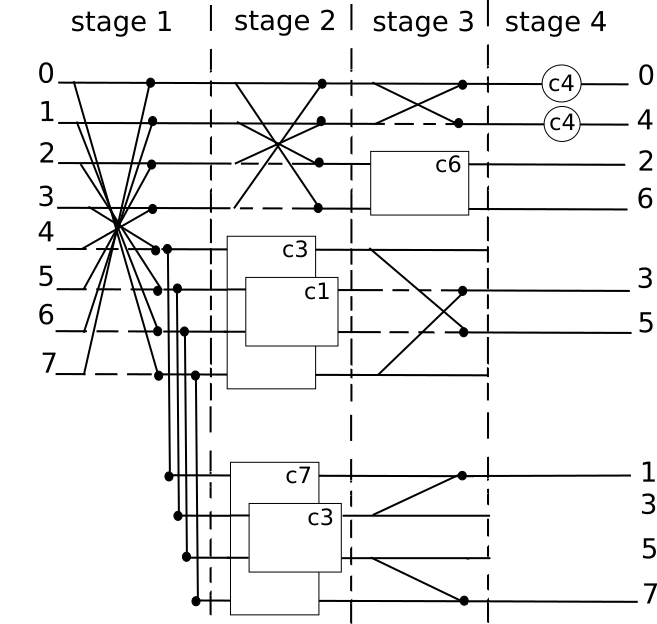
\includegraphics[width=\textwidth]{imm/dct/dct8.png} 	\caption{LLM DCT for an 8-point with 17 multiplications. For symbols, see figure \ref{dct8_scheme}} 
        	\label{dct8}
        \end{figure}

        The stages of the LLM Algorithm for an 8-point DCT, numbered 1 to 4, are parts that have to be executed in series and can not be evaluated in parallel because of data dependencies. However calculations inside one stage can be parallelized. \\
        Stage 1 consists of 8 additions/subtractions. \\
        In Stage 2 , the algorithm splits into two parts. One part is for even coefficients (only additions and subtractions) and the second part is for odd coefficients (rotations). \\
         The even part is nothing else than a 4-point DCT, again separating in even and odd part in stage 3.\\
         Figure \ref{dct8_scheme} explains the building blocks of the algorithm.  
     The second building block, the rotation, can be calculated using only 3 multiplications and 3 additions instead of 4 multiplications and 2 additions using the equivalence shown in equation \ref{rot_eq}.
     Since $ a=cos(\frac{n\pi}{2N}) $ and $ b=sin(\frac{n\pi}{2N}) $ are constants and known \textit{a priori}, also the values $ (b-a) $ and $ -(b+a) $ are constants, so we do not need an hardware component to compute them.
     \begin{equation}\label{rot_eq}
     \begin{aligned}
     	y_{0}\quad=&a\cdot x_{0} + b\cdot x_{1} \quad=& (b - a)\cdot x_{l}+a\cdot (x_{0}+x_{l})\\
     	y_{0}= & -b\cdot x_{0} + a\cdot x_{1}= &  -(b+a)\cdot x_{0}+a\cdot (x_{0}+x_{l})\\
     	a=&cos(\frac{n\pi}{2N})&\\
     	b=&sin(\frac{n\pi}{2N})&
     	\end{aligned}
     \end{equation}
     \bigskip
              \begin{figure}[h!]
              	\centering
              	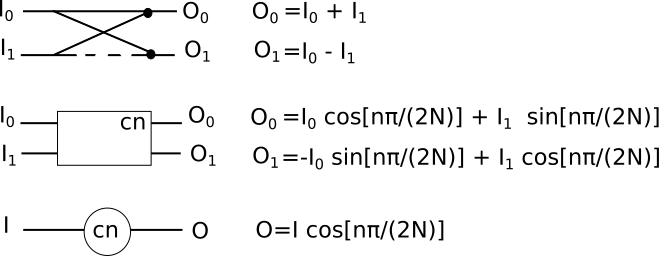
\includegraphics[width=\textwidth]{imm/dct/dct8_scheme.png} 	\caption{Symbols used to describe the LLM DCT for an 8-point with 17 multiplications (fig.\ref{dct8})} 
              	\label{dct8_scheme}
              \end{figure}
        
        
       
    \subsection{Simulation and test}
    I performed some tests of this implementation with different values. \\In the fig.\ref{tb_dct8} we can see the results of an array of 8 elements using the LLM structure.\\
    \bigskip
  \begin{figure}[h!]
              	\centering
              	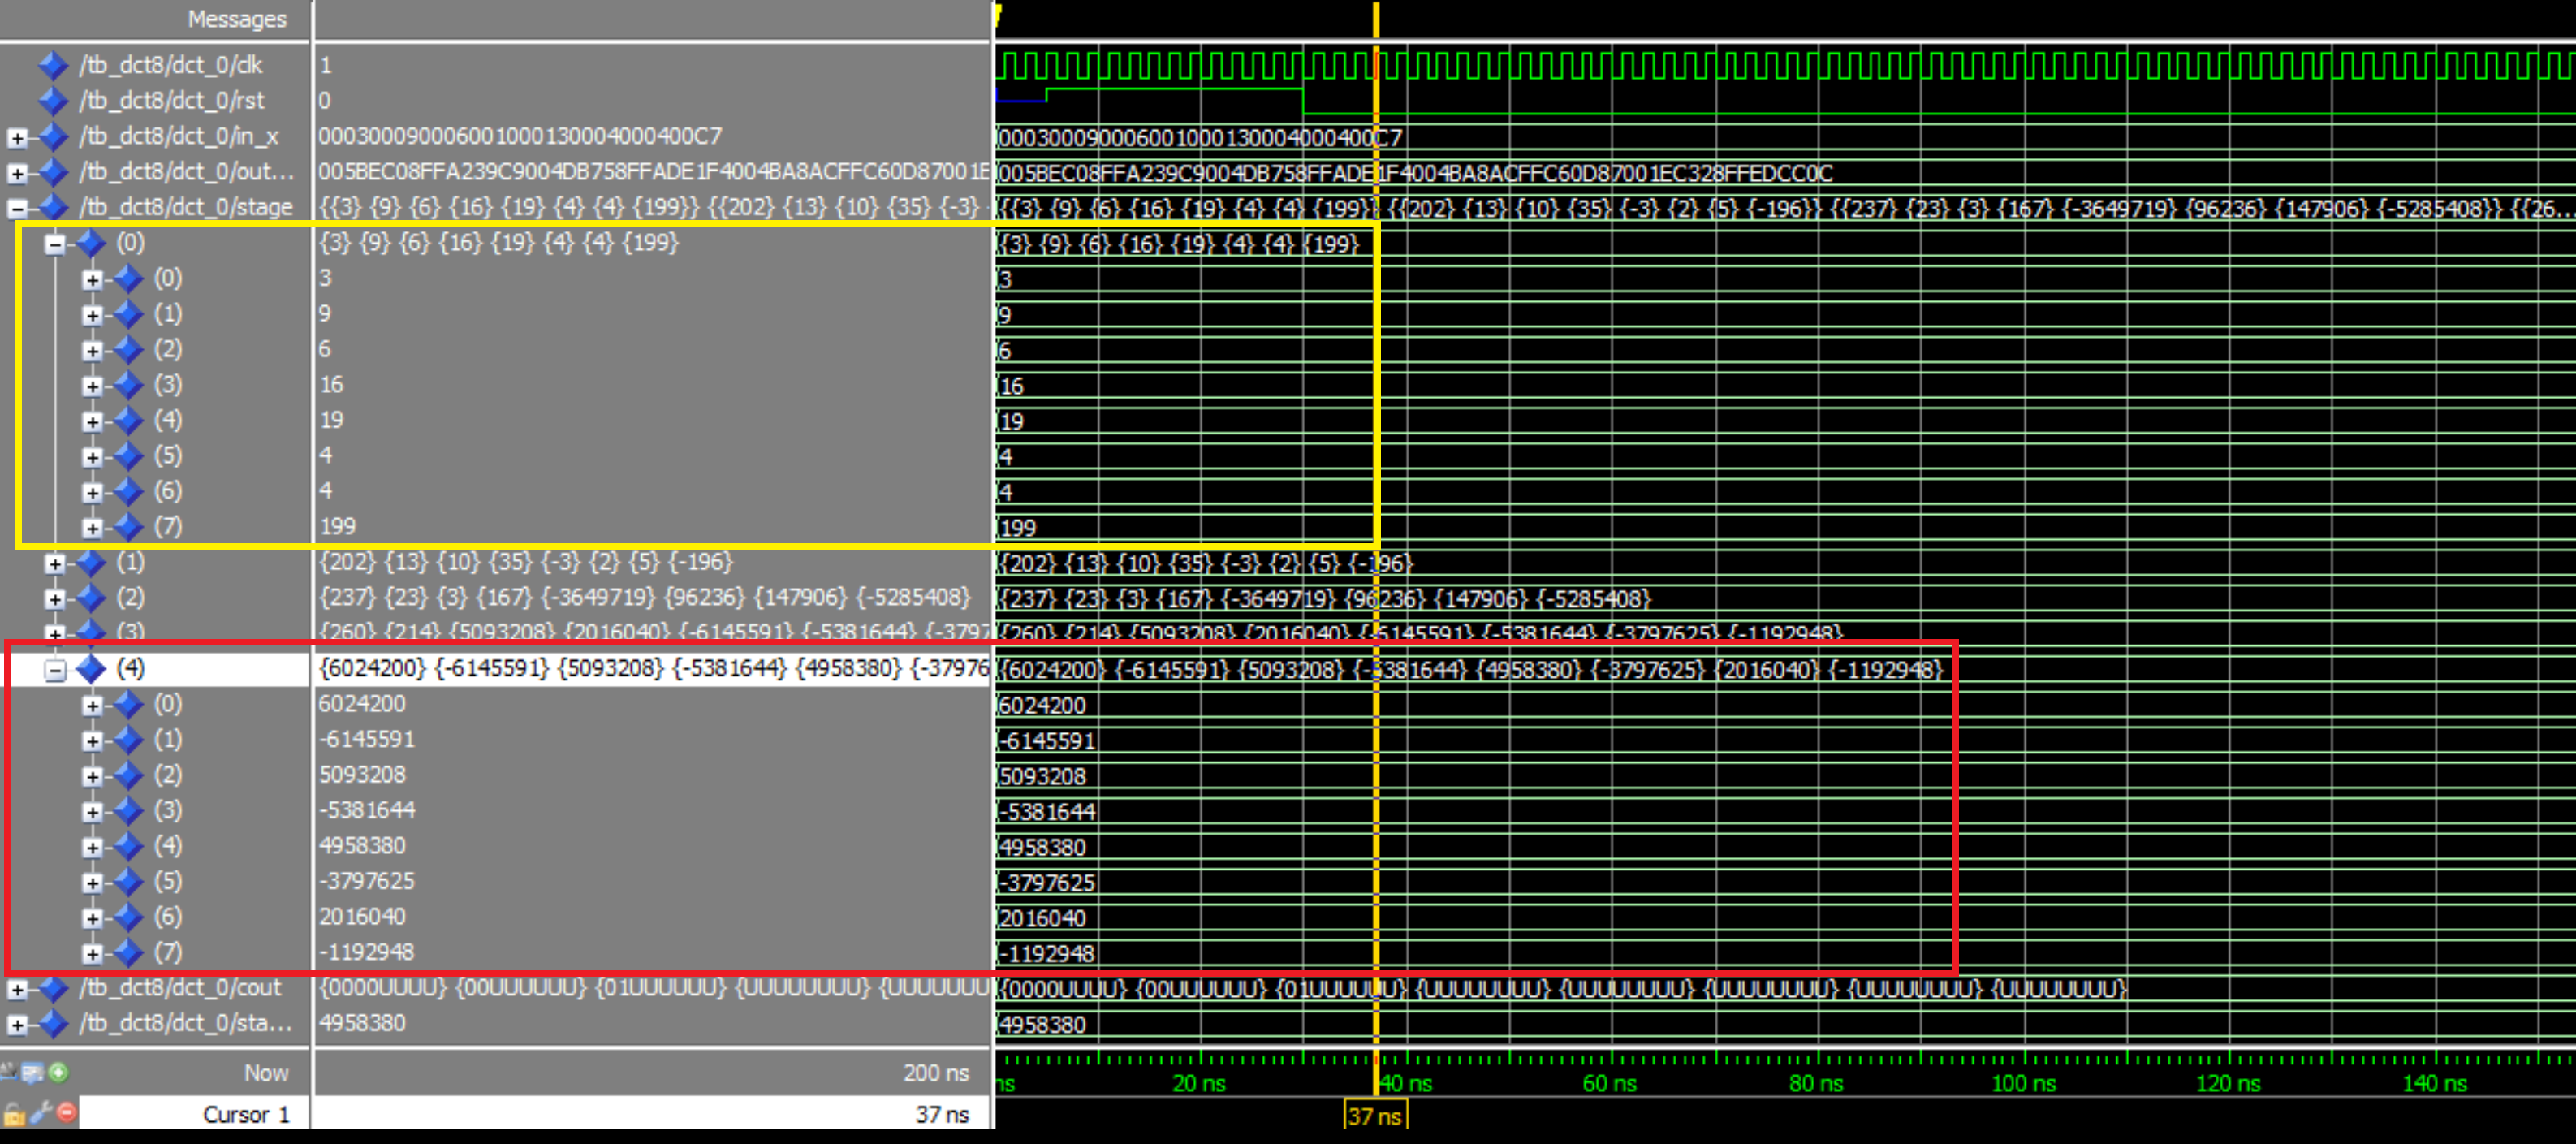
\includegraphics[width=\textwidth]{imm/dct/tb_dct8.png} 	\caption{LLM 8-point Discrete cosine transform-Results of the simulation} 
              	\label{tb_dct8}
  \end{figure}
  \bigskip
  In the yellow box, we can see the input vector to be
  \begin{center}
  		$ x_{0}=3$\\
  		$ 	x_{1}=9 $\\
  		$ x_{2}=6 $ \\
  		$ x_{3}=16 $ \\
  		$ x_{4}=19 $ \\
  		$x_{5}=4$\\
  			$x_{6}=4$\\
  				$x_{7}=199$\\
  \end{center}
  Between the yellow box and the red box, we can see the results of the different stages.\\
  The final result is shown in the red box. Since we reserved 16 bits for the decimal part, these vector has to be shifted by 16 position, i.e. divided by $ 2^{16}=65536 $.
  
    \begin{center}
    	$ X_{0}=6024200/2^{16}=91.9219$\\
    	$ X_{1}=-6145591/2^{16}=-93.7742 $\\
    	$ X_{2}=5093208/2^{16}= 77.7161$ \\
    	$ X_{3}=-5381644/2^{16}= -82.1173$ \\
    	$ X_{4}=4958380/2^{16}= 75.65887$ \\
    	$X_{5}=-3797625/2^{16}=-57.9471$\\
    	$X_{6}=2016040/2^{16}=30.7623$\\
    	$X_{7}=-1192948/2^{16}=-18.2029$\\
    \end{center}
     We checked this result by using the function $ dct $ on Matlab (Figure \ref{fig:dct8_res_mat}).
     We see that it differs from the Matlab result by a value in the order of 1/100. This depends on the precision used for the implementation, especially when converting the cosine values into binary.
     
     
     
     
     
     \begin{figure}[h!]
     	\centering	
     	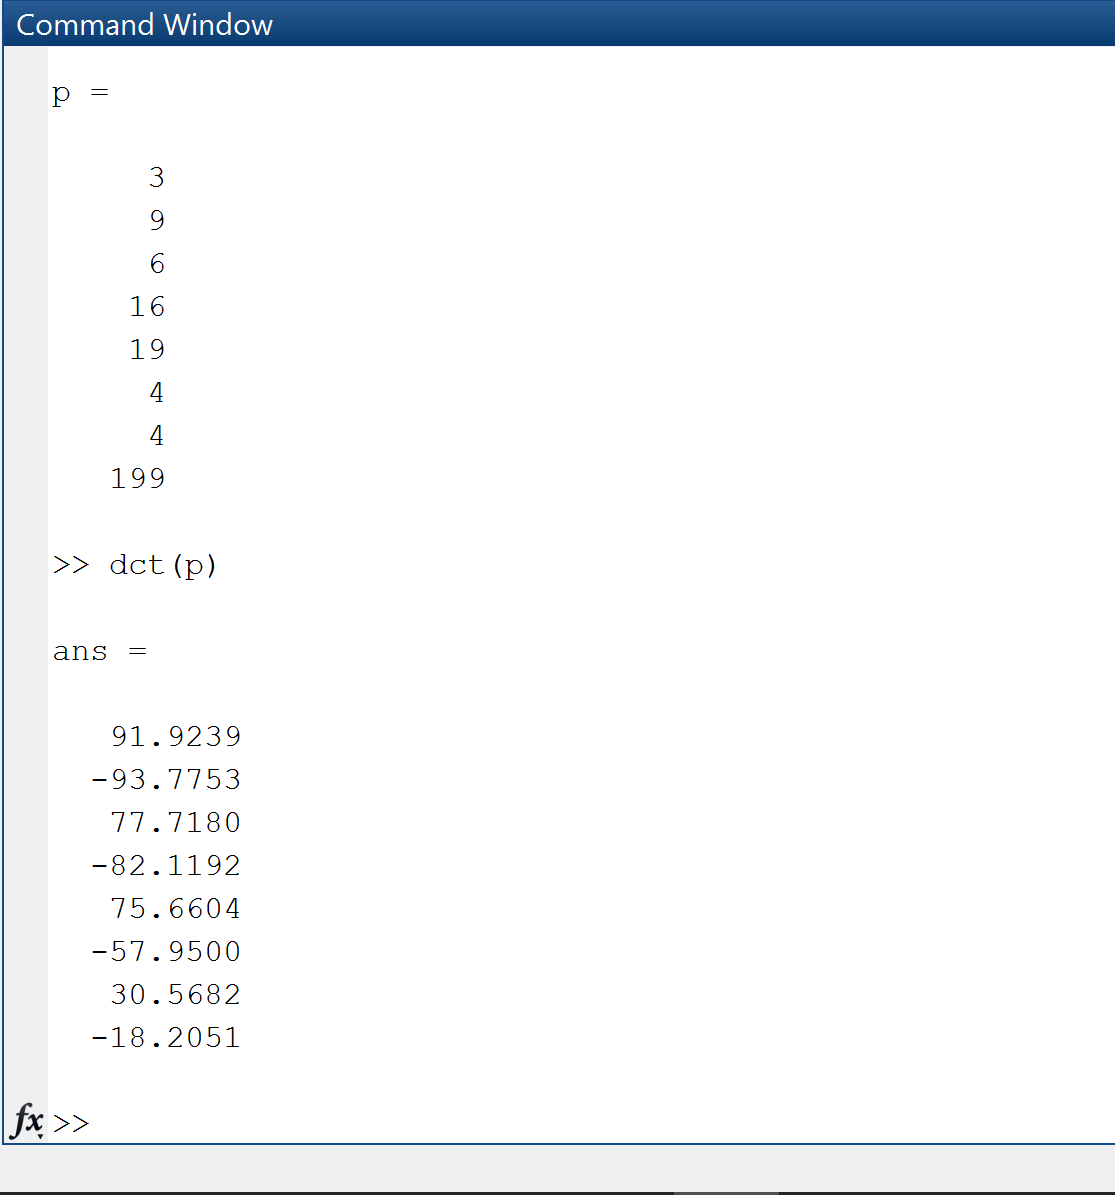
\includegraphics[width=0.9\textwidth]{imm/dct/dct8_matlab.png}  
     	\caption{LLM 8-point DCT result in MATLAB} 
     	\label{fig:dct8_res_mat}
     \end{figure}
     
     \subsection{Comparison}
     Since this architecture is fon an 8-point DCT, I will compare it with the other structure for the DCT shown before (subsection \ref{DCTH} and \ref{DCTSA}).
     \begin{center}
     	\begin{tabular}{ | p{1cm} |  p{2.5cm} |  p{2.5cm} | p{2.5cm} | p{2.5cm}|p{2.5cm}|}
     	\hline
     	\label{table:dct8_tab}N=8 & Systolic array & This work & This work pipelined & LLM & LLM pipelined\\
     	\hline
     	Area & $ 8^{2}$ \textit{multiplications} $8^{2}$ \textit{additions}&$8^{2}$ \textit{ moltiplications}  $ 8^{2}$\textit{additions} & $8$ \textit{moltiplications} $8$\textit{additions} & $17$ \textit{moltiplications} $33$\textit{additions} & $4.25
     	$ \textit{moltiplications}  $ 8.25$\textit{additions}\\ 
     	\hline
     	Time &$(2\cdot8-1)$ x \textit{(time for a multiplication followed by an addition)}&
     	$ 8 $ x \textit{(time for a multiplication followed by an addition)}&\textit{time for a multiplication followed by an addition}&\textit{time for 3 multiplications and 6 addition}&\textit{time for 1 multiplication and 2 additions}\\      	
     	\hline     
     		
     	\end{tabular}
     \end{center}
     \bigskip
     We can see that the LLM (both pipelined and not) is the best solutions in terms of area.\\
     In terms of time, if we look to the pipelined LLM architecture, we have to consider the longest critical path between the four stages. This is found in the rotation block, which takes the time for a multiplication and 2 additions. The Data Flow Graph is shown in fig. \ref{rot}.
          \begin{figure}[h!]
          	\centering	
          	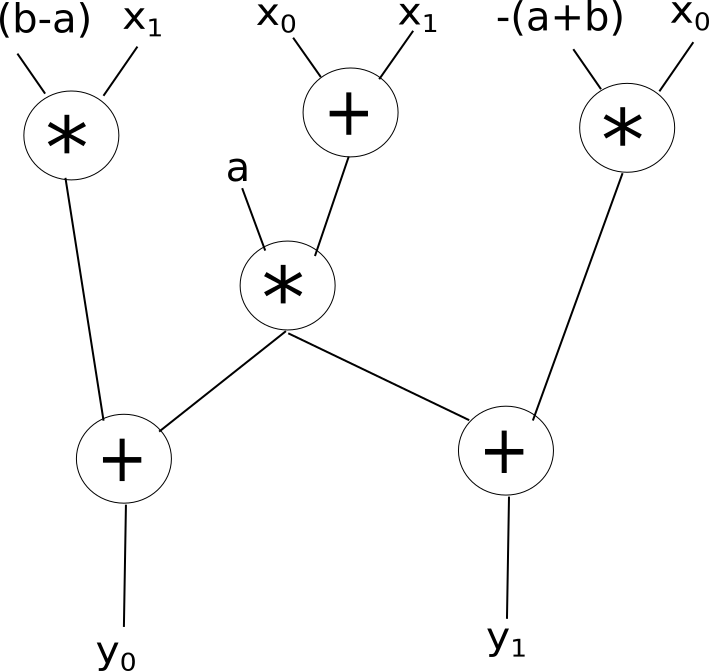
\includegraphics[width=0.7\textwidth]{imm/dct/rot.png}  
          	\caption{DFG for a rotation block} 
          	\label{rot}
          \end{figure}
     So looking to the pipelined architectures of the LLM and the one shown in this work (subsection \ref{DCTH}), it's better the one i presented above.\\
     If we look to the architecture without any pipeline register, the critical path will be 1 multiplication and 4 additions. To find this value, we can consider the critical path for each output element, by taking into account that a rotation block take the time for one multiplication and 2 additions.
     A scheme is shown in fig. \ref{dfg_llm}.
               \begin{figure}[h!]
               	\centering	
               	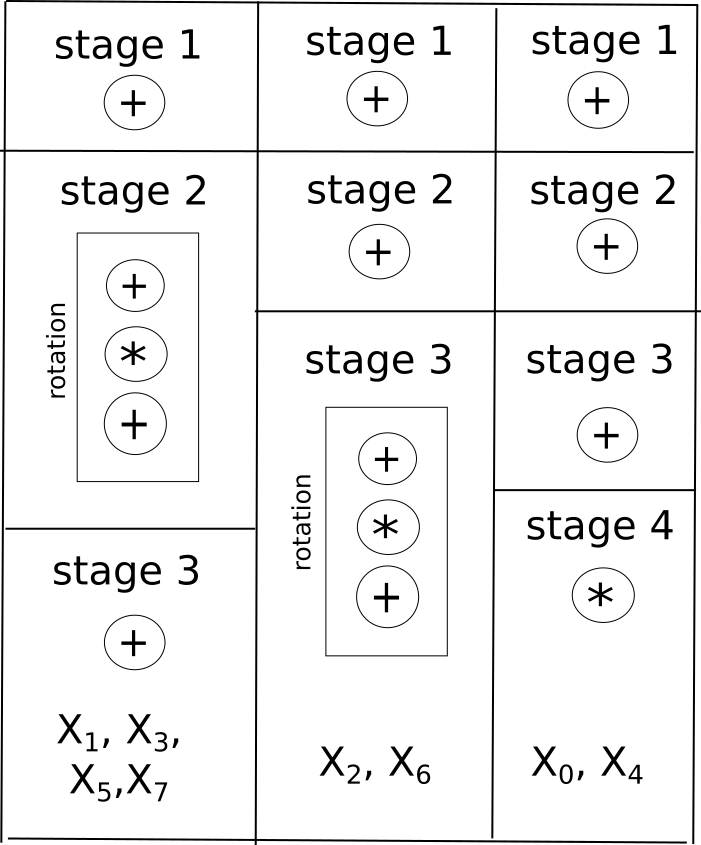
\includegraphics[width=\textwidth]{imm/dct/dfg_llm.png}  
               	\caption{Critical path for each output element} 
               	\label{dfg_llm}
               \end{figure}
      In conclusion, without any pipeline registers, it's better the LLM architecture in terms of time.
 
          \clearpage        
          \newpage
          \subsection{High Order LLM DCT} \label{HLLM}
          Many studies has been done for the LLM architecture, and it has been theorized that the LLM can be applied for the DCT that has a size of $ 2^{n}$. \cite{llm1}\\
 Although we can see a recursive approach for the even parts at top, such as an addition/substraction, nothing can be said for the odd parts. A brute-force search is required. \cite{llm2}\\
 Fig. \ref{dct16} and fig. \ref{dct32} show an implementation for the LLM of order-16 and order-32 respectively.  
\begin{figure}[h!]
     	\centering	
     	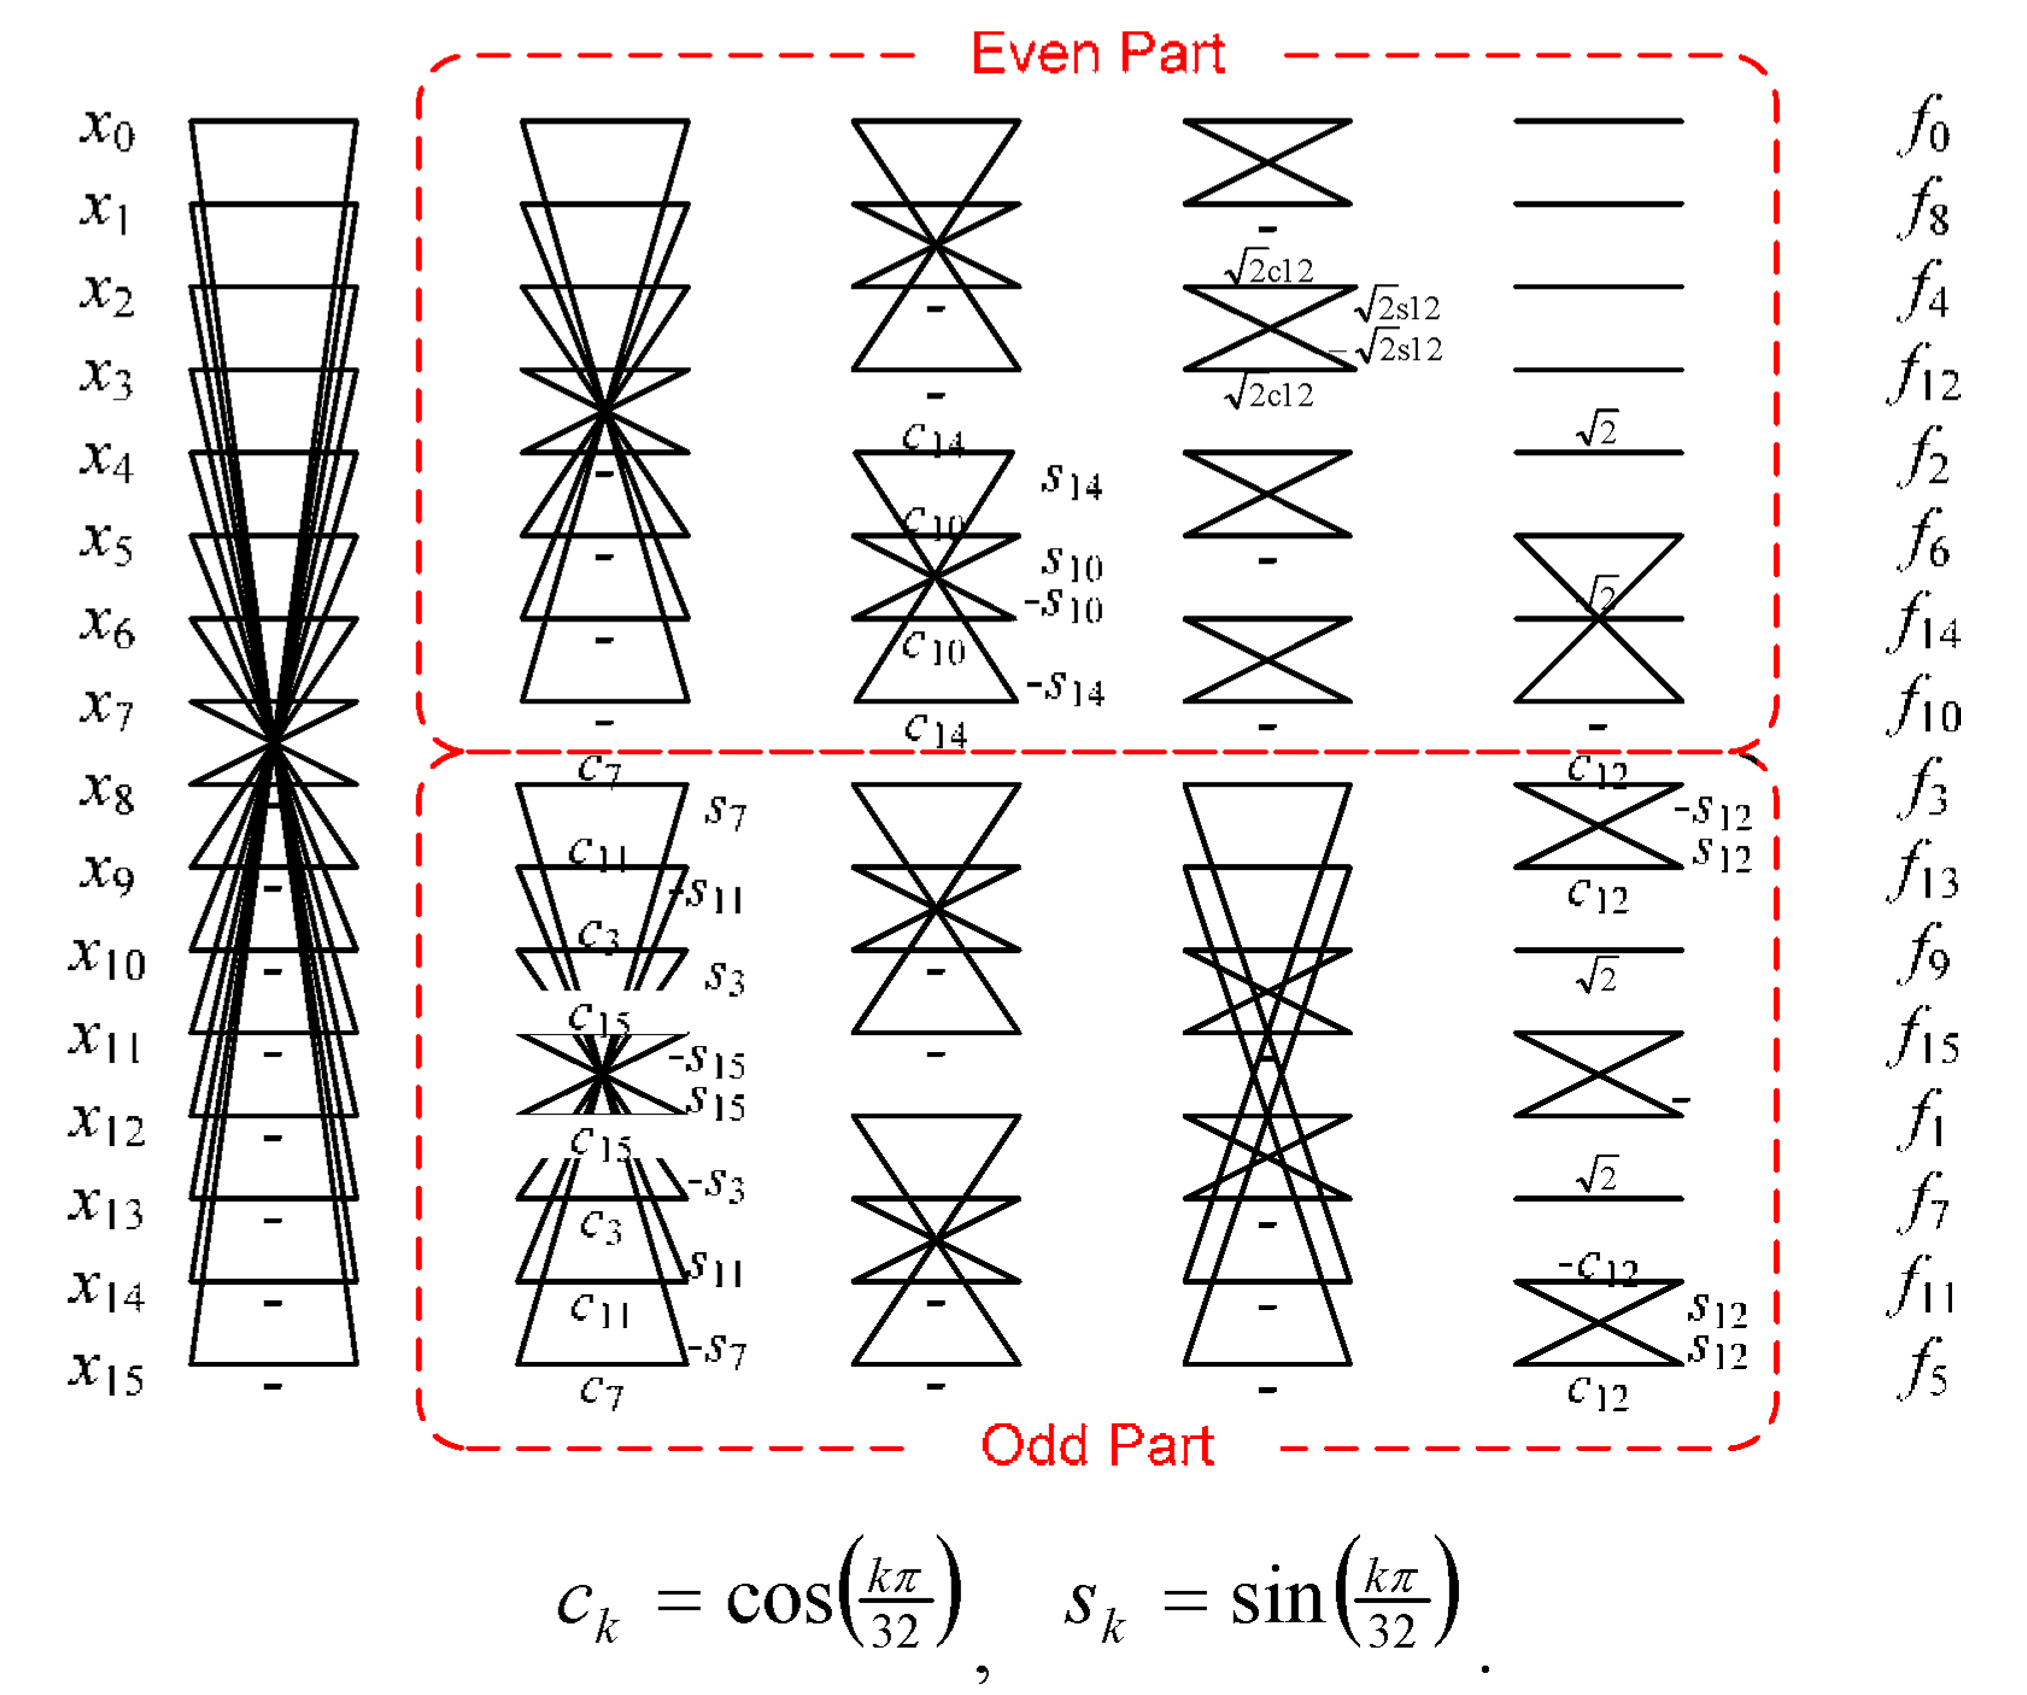
\includegraphics[width=\textwidth]{imm/dct/dct16.png}  
     	\caption{Order-16 LLM fast DCT algorithm} 
     	\label{dct16}
\end{figure} 

\begin{figure}[h!]
     	\centering	
     	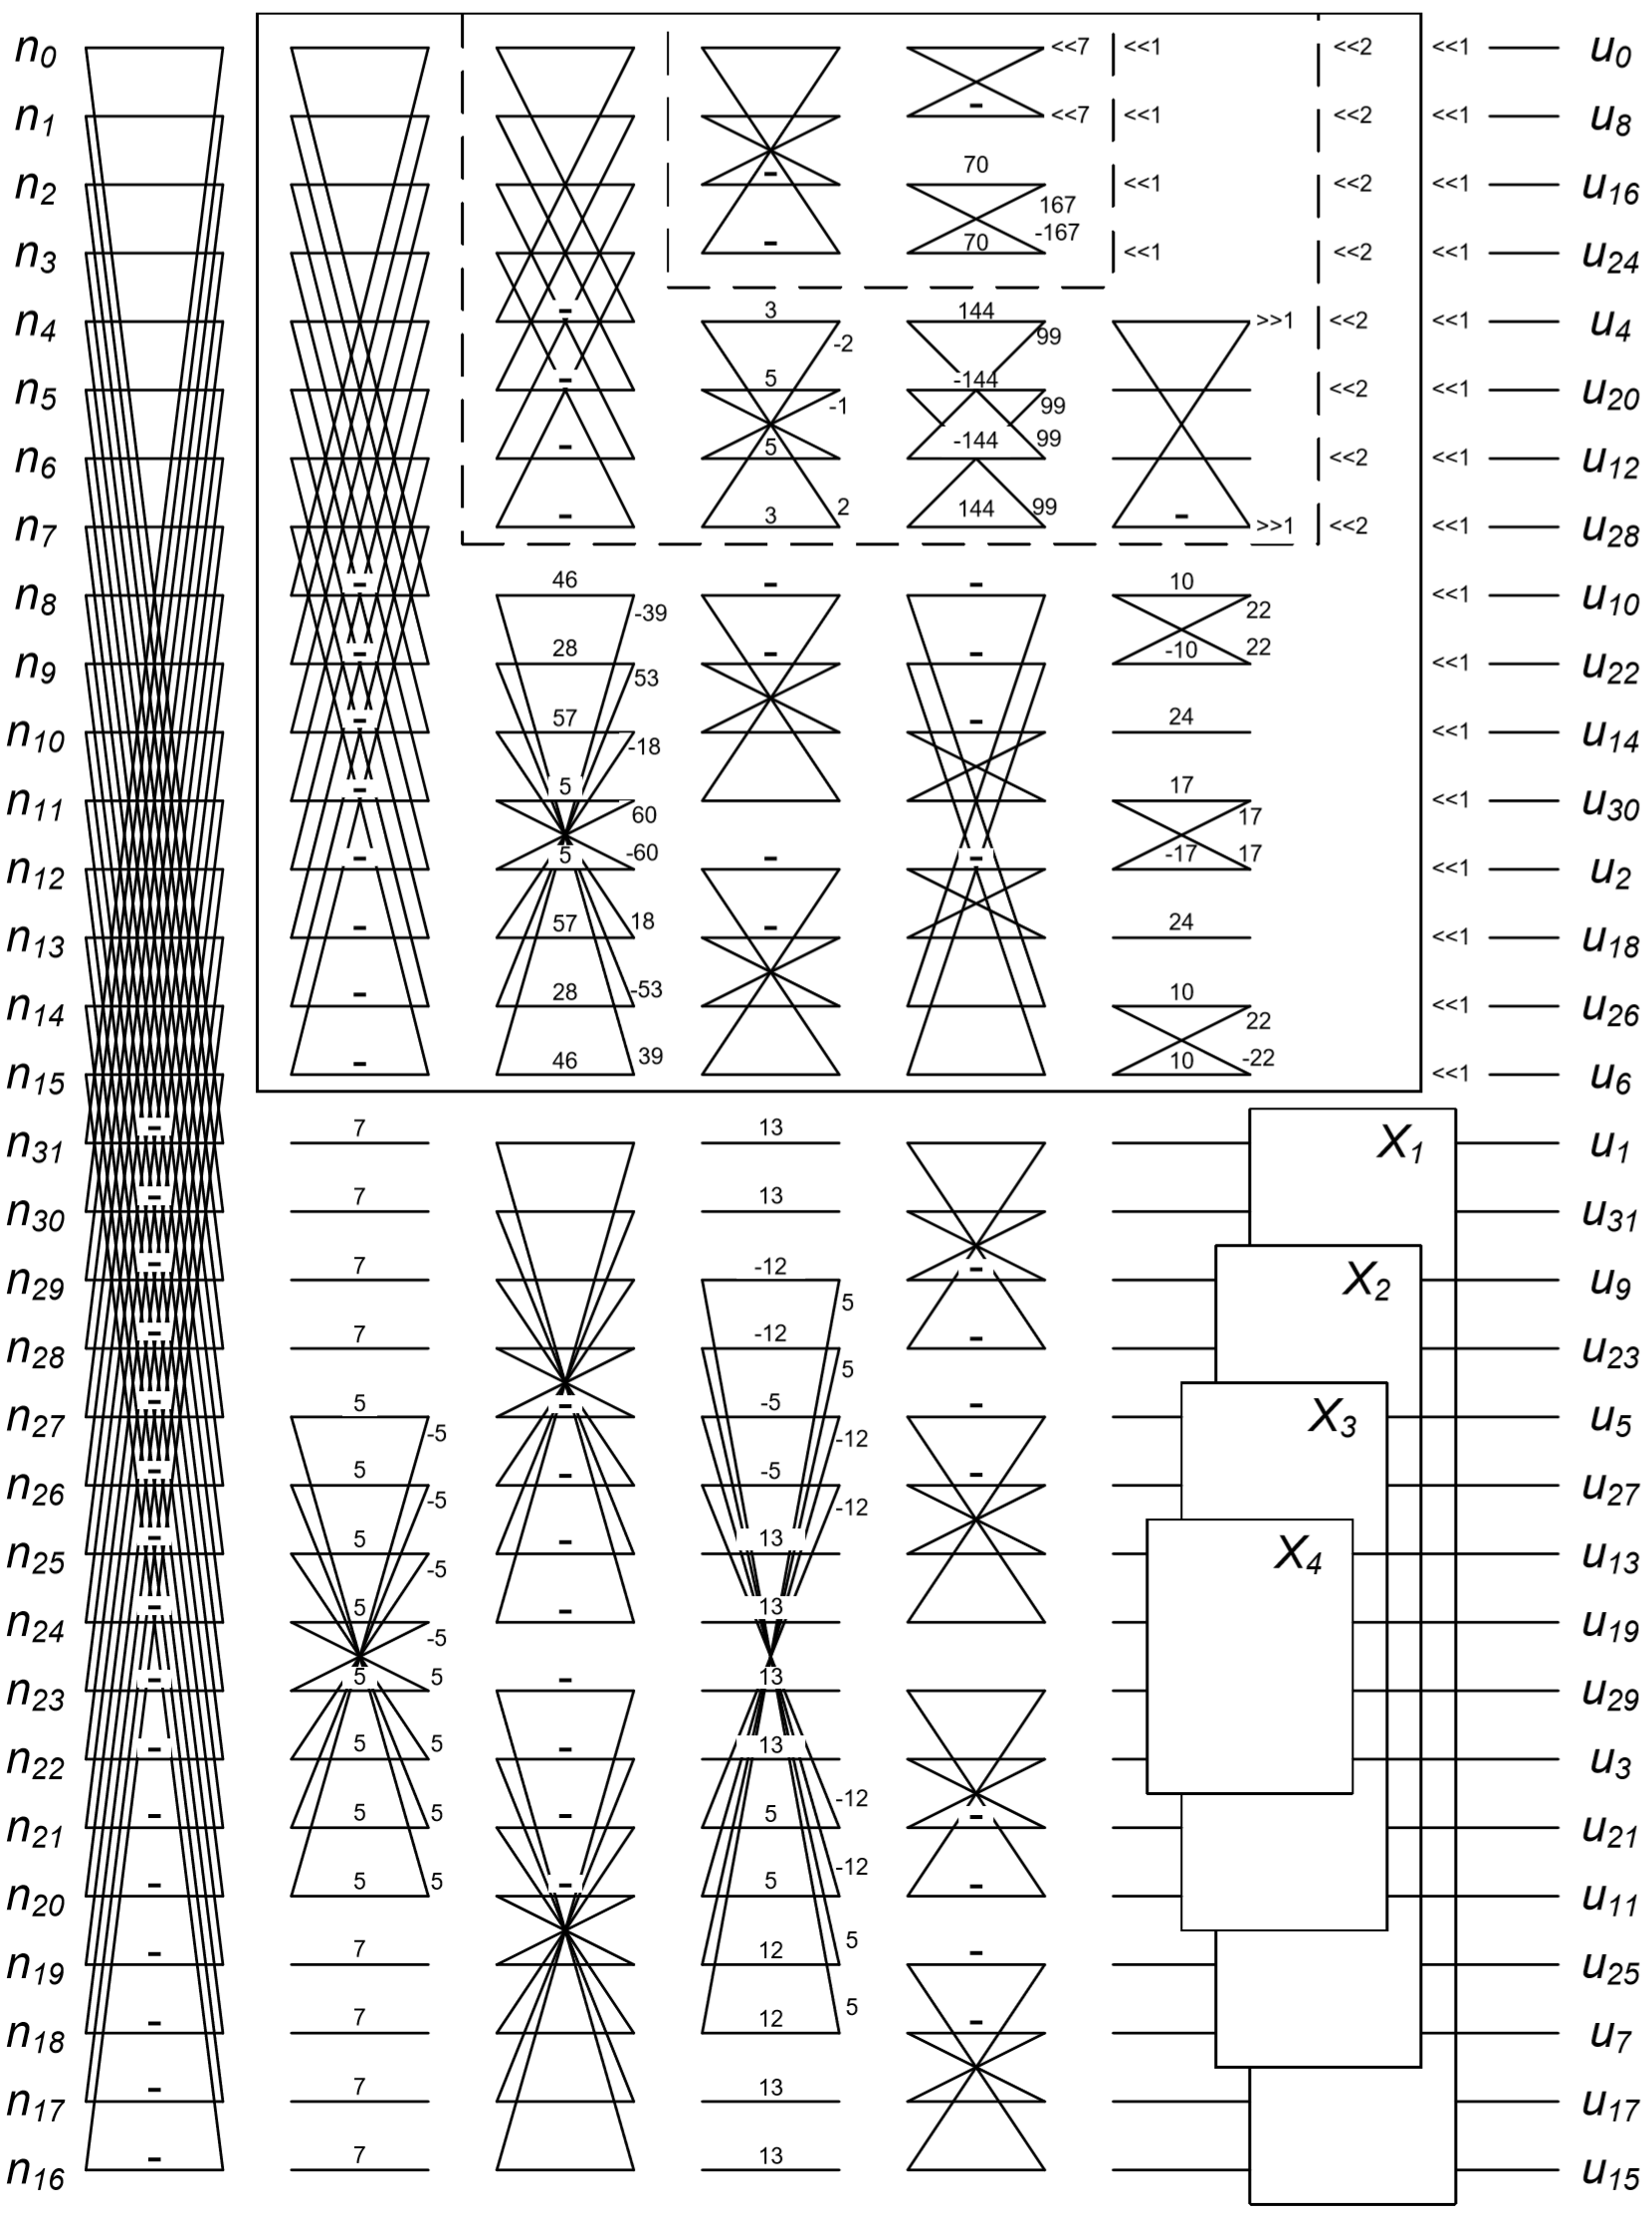
\includegraphics[width=\textwidth]{imm/dct/dct_2n.png}  
     	\caption{ Fast algorithm for the forward order-32 integer transform with the fast algorithms for the forward order-4, order-8, and order-16 integer transforms embedded. } 
     	\label{dct32}
\end{figure}  

\clearpage        
\subsection{Characteristics of the LLM DCT 8-point}
\vspace{10pt}
{\large \textbf{PROCESSING ELEMENTS}}\vspace{10pt}\\
\begin{tabular}{ p{0.2cm} p{14.5cm}}
	
	&\textbf{1- Which kind of Processing element?}\\
	&	Adder, multiplier, substractor\vspace{7pt}\\
	&	\textbf{2- Functionality}\\
	&	Addition, mulltiplication, substraction, summation\vspace{7pt}\\
	&	\textbf{3- Complexity}\\
	&	\begin{tabular}{ p{0.2cm} p{2.5cm} p{10cm}}
		
		&Not pipelined & Area: \quad $ 17 $ multiplier, $ 33 $ additions\\
		& & Time:\quad8x(time for 3 multipliers and 6 adders) \vspace{3pt}\\
		& Pipelined & Area: \quad $ 4.25$ multiplier, $ 8.25$ additions\\
		& & Time:\quad time for a multiplication and by 2 additions\\
		
	\end{tabular}\vspace{7pt}\\
	&	\textbf{4- Parallelism}\\
	& Each operation belonging in a certain phase, can be done in parallel. (Fig. \ref{dct8})\vspace{7pt}\\
	&	\textbf{5-Reconfigurability}\\
	&	No\vspace{7pt}\\
	&	\textbf{6- Programmability}\\
	&	No\vspace{7pt}\\
	&	\textbf{7- Need a dedicated memory?}\\
	&	Yes, it needs to store the cosine values.\\
	&	If not pipelined, no memory is required.\vspace{7pt}\\
	&\textbf{8- Relationship with I/O}\\
	&	INPUT: values of the input vector\\
	&	OUTPUT: result of the DCT algorithm\end{tabular}\vspace{74pt}\\
\newpage{\large \textbf{\qquad }}\vspace{10pt}\\
{\large \textbf{MEMORY ELEMENTS}}\vspace{5pt}\\\begin{tabular}{ p{0.2cm} p{14.5cm}}
	&\textbf{1- Need a clever memory LIM?}\\
	&	No\vspace{7pt}\\
	&\textbf{2- Is there a data search algorithm?}\\
	&	No\vspace{7pt}\\
	&\textbf{	3-Interface mechanism with other PE or memories}\\
	&	Communication required between local cells\vspace{7pt}\\
	&	\textbf{4- Access mechanism}\\
	&	(No memory for this implementation)\vspace{7pt}\\
	&	\textbf{5- Hierarchization} \\
	&	(No memory for this implementation)\vspace{7pt}\\
	&\textbf{	6- Cache coherency} \\
	&	(No memory for this implementation)\vspace{7pt}\\
	&\textbf{	7- Is it a a transactional memory?}\\
	&	(No memory for this implementation)\vspace{7pt}\\
	&\textbf{	8- Are there virtualization (paging) mechanisms?}\\
	&	(No memory for this implementation)\end{tabular}\vspace{14pt}\\
\vspace{10pt}\\
{\large\textbf{ENCODING INFORMATION}}\vspace{10pt}\\
\begin{tabular}{ p{0.2cm} p{14.5cm}}
	&\textbf{1-Which encoding is used?}\\
	&Binary encoding (by reserving some bits for the decimal part) for the cosine matrix and for the result
\end{tabular}
\newpage{\large\textbf{ }}\vspace{10pt}\\
{\large\textbf{CONNECTIONS}}\vspace{10pt}\\\begin{tabular}{ p{0.2cm} p{14.5cm}}
	&\textbf{1-Packet Exchange Protocol}\\
	&Directly\vspace{7pt}\\
	&\textbf{2-Timing (asynchronou/synchronous)}\\
	&Synchronous\vspace{7pt}\\
	&\textbf{3-Are there multiple instances? }\\
	&Yes, but the architecture is not simmetric (\ref{dct8})\vspace{7pt}\\
	&\textbf{4-Heterogeneity (Local/Distant I/O Connections)}\\
	&Heterogeneous when storing the values of the input vector.\vspace{7pt}\\
	&\textbf{5-Are there any buffers?}\\
	&There are pipeline registers.
\end{tabular}\vspace{14pt}\\

%  \chapter{Binomial Filter}
   Binomial filters are simple and efficient structures based on the binomial coefficients for implementing Gaussian filtering. 
   To extract these coefficients, we could use Pascal's Triangle.\\
   The rows of Pascal's triangle are conventionally enumerated starting with row $ n = 0 $ at the top (the 0\^{th} row). The entries in each row are numbered from the left beginning with $ k = 0 $ and are usually staggered relative to the numbers in the adjacent rows. The triangle may be constructed in the following manner: In row $ 0 $ (the topmost row), there is a unique nonzero entry$  1 $. Each entry of each subsequent row is constructed by adding the number above and to the left with the number above and to the right, treating blank entries as $  0 $. For example, the initial number in the first (or any other) row is $ 1  $(the sum of $ 0 $ and $ 1 $), whereas the numbers $ 1 $ and $ 3 $ in the third row are added to produce the number $ 4 $ in the fourth row.
   \bigskip
\begin{center}
	  \begin{tabular}{>{$n=}l<{$\hspace{15pt}}*{13}{c}}
  	0 &&&&&&&1&&&&&&\\    1 &&&&&&1&&1&&&&&\\    2 &&&&&1&&2&&1&&&&\\    3 &&&&1&&3&&3&&1&&&\\    4 &&&1&&4&&6&&4&&1&&\\    5 &&1&&5&&10&&10&&5&&1&\\    6 &1&&6&&15&&20&&15&&6&&1
  \end{tabular}
\end{center}
\bigskip
The first  odd sized serie is:
 \begin{center}
	1 \quad 2 \quad 1\\
\end{center}
 this form the basis for the 3x3 binomial filter. \\
 The weights of the binomial filter are biggest at the center and taper down towards the outer areas of the neighborhood. \\ 
 To create the 2D low pass binomial filter, we have to form the outer product of the row with its corresponding column. In simple terms take the row and multiply each element in it by the first value in the row. Then take the row and multiply each element in it by the second value in the row. Repeat this until we have multiplied the row by every element in the row. Then stack each of these resulting rows to make a square table or matrix. \\
 For example, the 3x3 matrix is generated as 
   \begin{center}
   	$ \begin{bmatrix}1\\ 2 \\ 1 \end{bmatrix} \cdot
   	\begin{bmatrix} 1 & 2 & 1 \end{bmatrix}= \begin{bmatrix}1 & 2 & 1\\
   	2 & 4 & 2   	\\1 & 2 & 1\end{bmatrix}$
   \end{center}
      After multipling, we need to normalize, so the overall 3x3 binomial filter is:
   \begin{center}
   	$   \dfrac{1}{16}\begin{bmatrix}1 & 2 & 1\\
   	2 & 4 & 2   	\\1 & 2 & 1\end{bmatrix}$
   \end{center}
    In particular, given a cell in position $ (x, y) $, the final value of the computation should be:
   
     \begin{equation} \label{eq:BN eq}
     \begin{aligned}
     f(x,y)= \dfrac{1}{16} & [  1(x-1,y-1) + 2(x-1,y)+ 1(x-1, y+1)+\\
     & + 2(x,y-1) + 4(x,y)+ 2(x, y+1)+\\
     & + 1(x+1,y-1) + 2(x+1,y) + 1(x+1, y + 1) ] \\
     \end{aligned}
     \end{equation}
     
     As shown in the figure below, the value of the dark blue rectangle can be calculated as the weighted mean of all the light blue rectangles:
       
        \begin{figure}[h!]
        	\centering
        	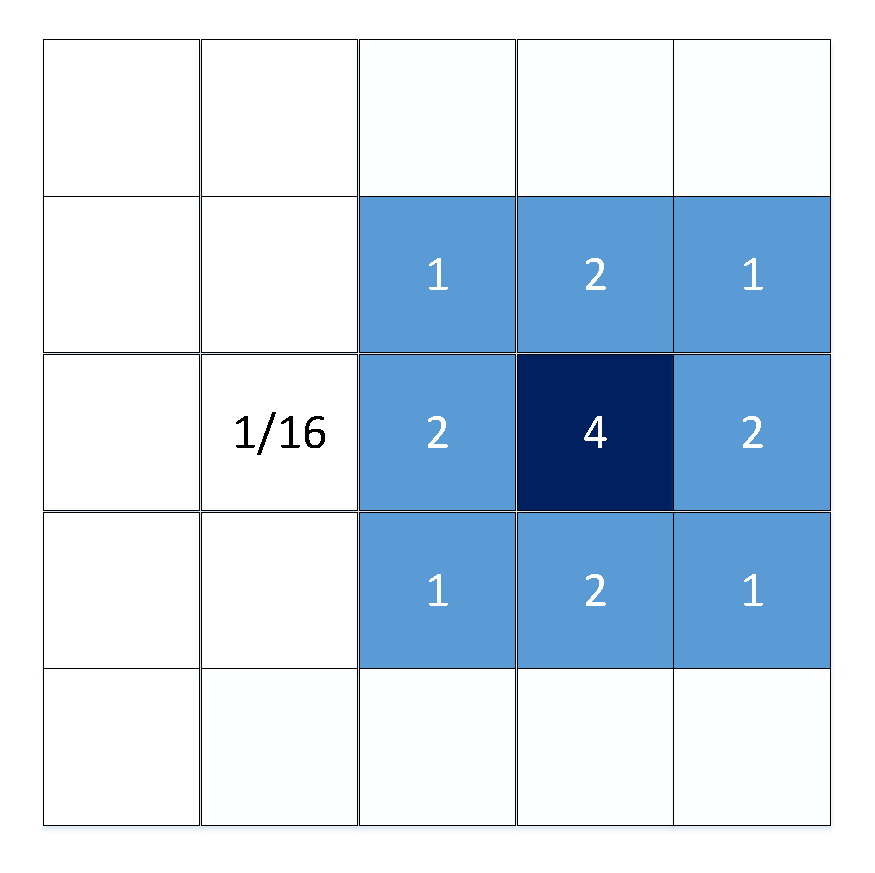
\includegraphics[width=\textwidth]{imm/bf/bf1.pdf} 	\caption{Binomial Filter for a generic cell} 
        	\label{fig:bf1}
        \end{figure}
        \clearpage
        \section{Hardware implementations} \label{bfh}
        \subsection{Hardware implementation type 1} \label{h1}
        This implementation will focus only to the possible cells for the binomial filter, i.e. the ones not in the border of the matrix, bevause they are leaved unchanged.
        \begin{enumerate}
        	\item for each row, whenever we find three consecutive cells, we evaluate the sum \begin{center}
        		$ S_{x,y}=cell_{x-1,y}+2\cdot cell_{x,y}+cell_{x+1,y}$
        	\end{center}
        	In order to so, we need 2 adder: we shift by one position the value of the central cell (i.e. multiply by two) and sum it with the left and the right cells as shown in fig \ref{fig:bflev11} while fig \ref{fig:bflev1} shows the overall picture of this step.
        	\begin{figure}[h!]
        		\centering
        		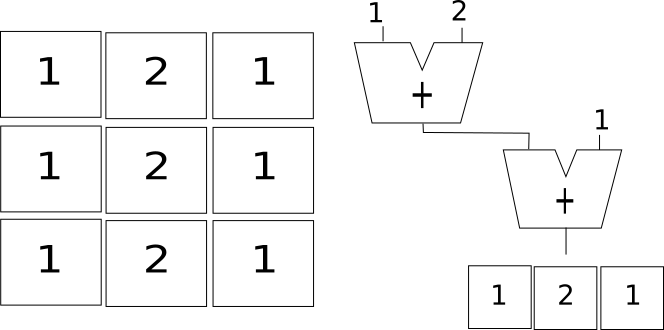
\includegraphics[width=\textwidth]{imm/bf/bflev11.png}  
        		\caption{Weighted sum for three consecutive cells} 
        		\label{fig:bflev11}
        			\end{figure}
        			
        	\begin{figure}[h!]
        		\centering
        		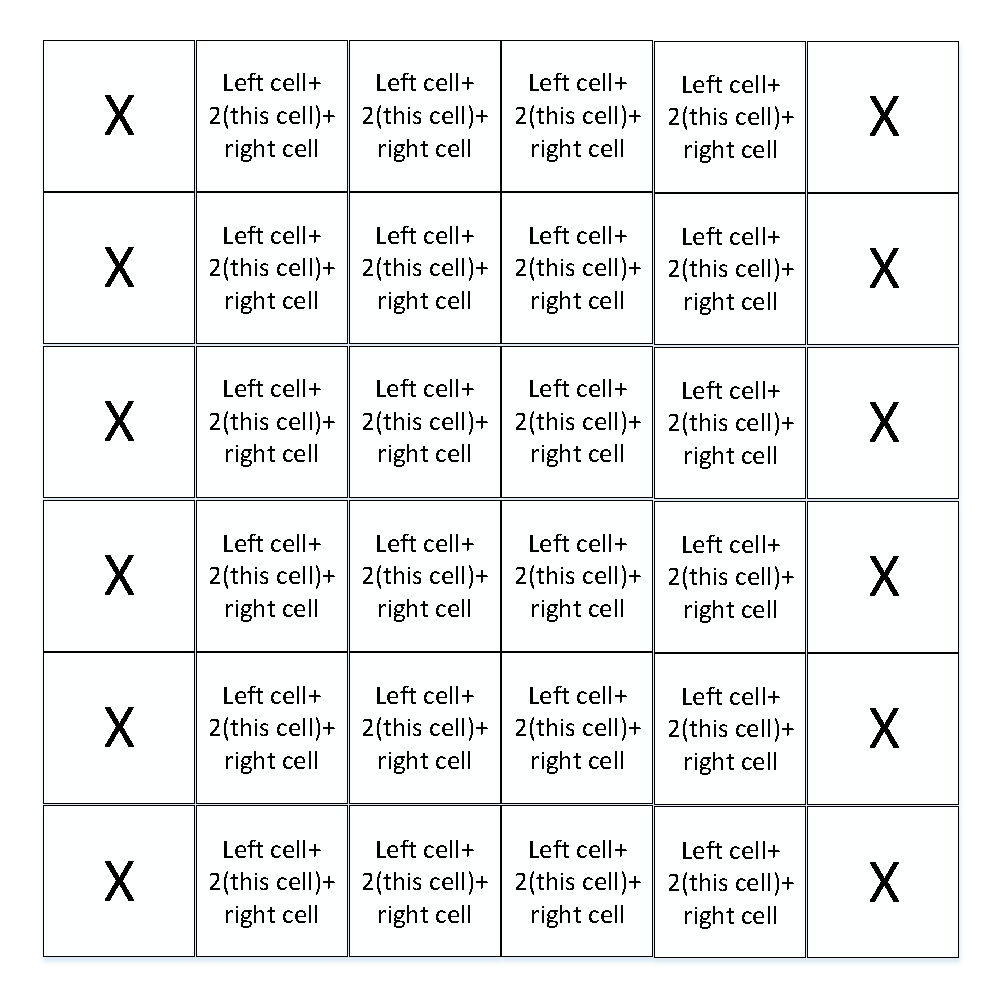
\includegraphics[width=\textwidth]{imm/bf/bflevel1.pdf}  
        		\caption{First part of the binomial filter HW implementation} 
        		\label{fig:bflev1}
        	\end{figure}
        	\clearpage
        	\item Taking the result of the previous step as a matrix, for each column whenever we found three consecutive cells we evaluate the sum
        	\begin{center}
        			$ SUM_{x,y}=S_{x,y-1}+2\cdot S_{x,y}+S_{x,y+1}$
        	\end{center}
        	which is equal to 
        	\begin{equation} \label{eq:BF_eq}
        	\begin{aligned}
        SUM_{x,y} =& (cell_{x-1,y-1}+2\cdot cell_{x,y-1}+cell_{x+1,y-1})+\\
        & +2\cdot (cell_{x-1,y}+2\cdot cell_{x,y}+cell_{x+1,y})+\\
        &+(cell_{x-1,y+1}+2\cdot cell_{x,y+1}+cell_{x+1,y+1}) =\\
        =& cell_{x-1,y-1}+2\cdot cell_{x,y-1}+cell_{x+1,y-1}+\\
        &+ 2\cdot cell_{x-1,y}+4\cdot cell_{x,y}+2\cdot cell_{x+1,y}+\\
        &+ cell_{x-1,y+1}+2\cdot cell_{x,y+1}+cell_{x+1,y+1}
        	\end{aligned}
        	\end{equation}
        	fig \ref{fig:bflev12} shows this step
        	\bigskip
       	\begin{figure}[h!]
       		\centering
       		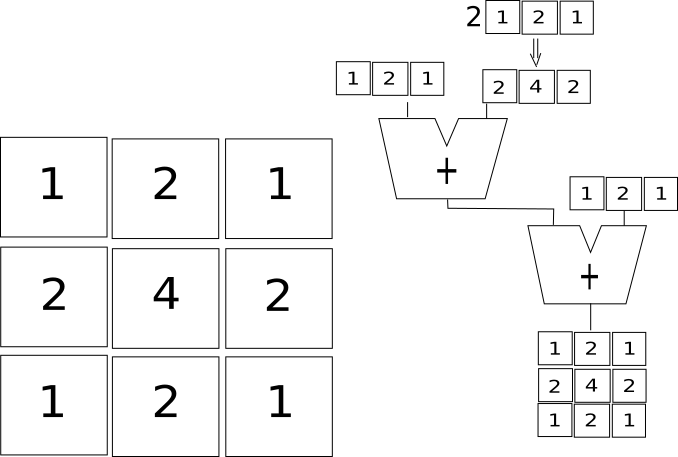
\includegraphics[width=0.95\textwidth]{imm/bf/bflev12.png}  
       		\caption{Weighted sum for 3x3 cells} 
       		\label{fig:bflev12} 	
        \end{figure}
        	\begin{figure}[h!]
        		\centering
        		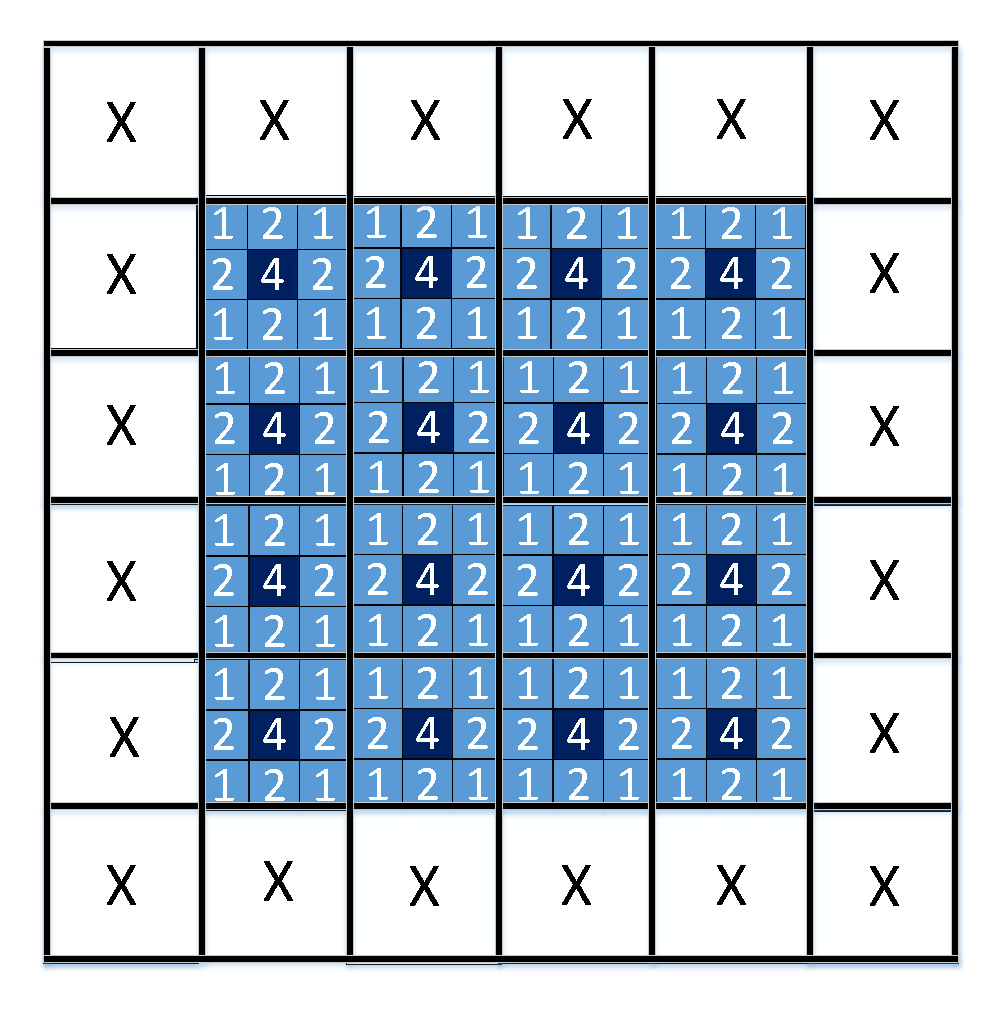
\includegraphics[width=\textwidth]{imm/bf/bflev2.pdf}  
        		\caption{Weighted sum for all 3x3 cells} 
        		\label{fig:bflev2}
        	\end{figure}
        \item Now that we have the weighted sum for all the 3x3 cells, we have to divided by 16. In order to do so, the quickest way is to shift the result by 4 bits.
        The values of the cells in the border of the matrix, are unchanged in the final result.
        	\end{enumerate}
     \clearpage
     \subsection{Hardware implementation type 2} \label{h2}
     This implementation will focus to all the cells. 
     The only difference between this implementation and the one  described in the subsection \ref{h1} is that now we apply the Binomial Filter also for the cells in the border of the matrix.
     We take the original matrix and we set a neighborhood of cells at $ '0' $ as shown in fig \ref{fig:h2} where the original matrix has benn highlighted in black.
     The procedure to evaluate the final result of the binomial filter is the same as explained in the subsection  \ref{h1}.
      \begin{figure}[h!]
      	\centering	
      	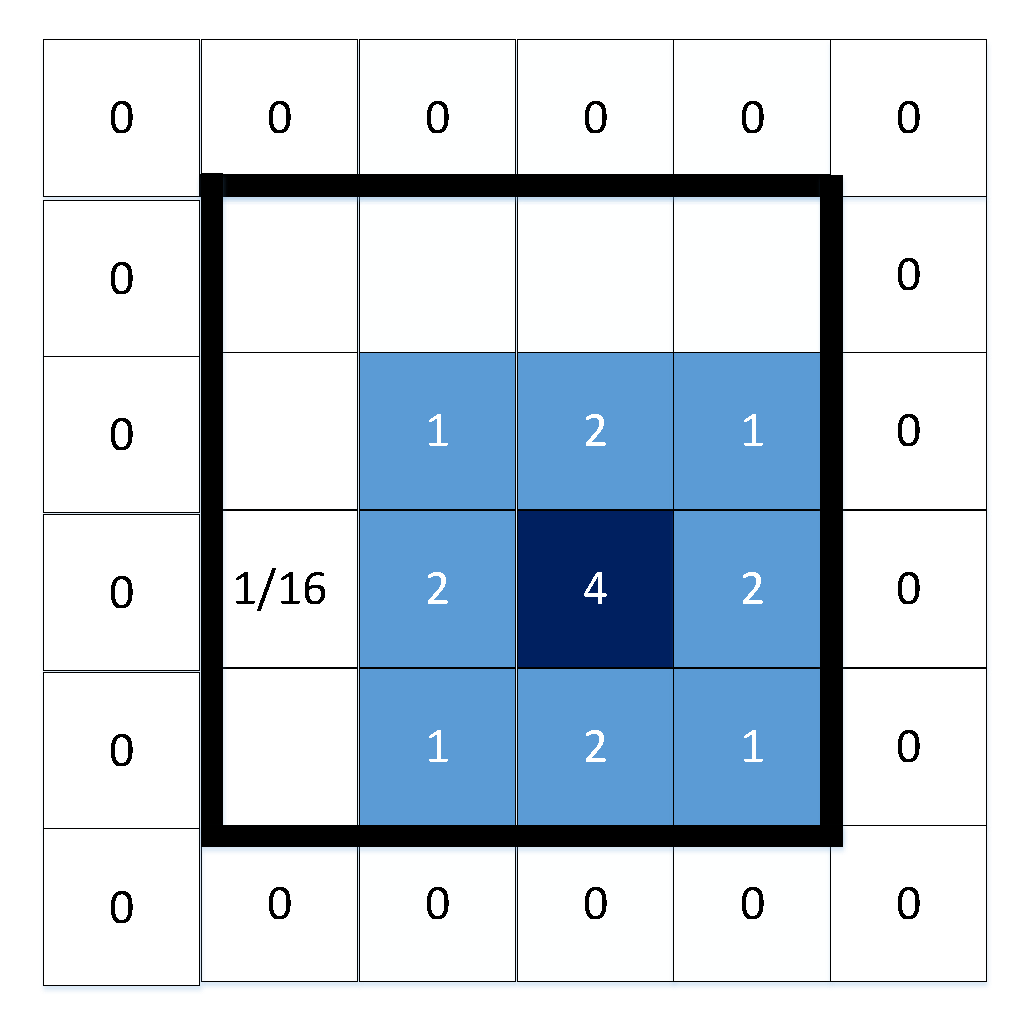
\includegraphics[width=0.9\textwidth]{imm/bf/bf_h2.pdf}  
      	\caption{Binomial Filter, second implemetation} 
      	\label{fig:fig:h2}
      \end{figure} 
     \section{Simulations}   
     \subsection{Simulation type 1} \label{sim1}
     The simulation shown in this work is referred to the hardware implementation descrived in the subsection \ref{h1} where the values of the matrix's border are leaved unchanged.
     In this testbench, we have a matrix 4x4 (fig.\ref{fig:tb_bf} highlighted in yellow, and the output highlighted in red).
    
     
     \begin{figure}[h!]
     	\centering	
     	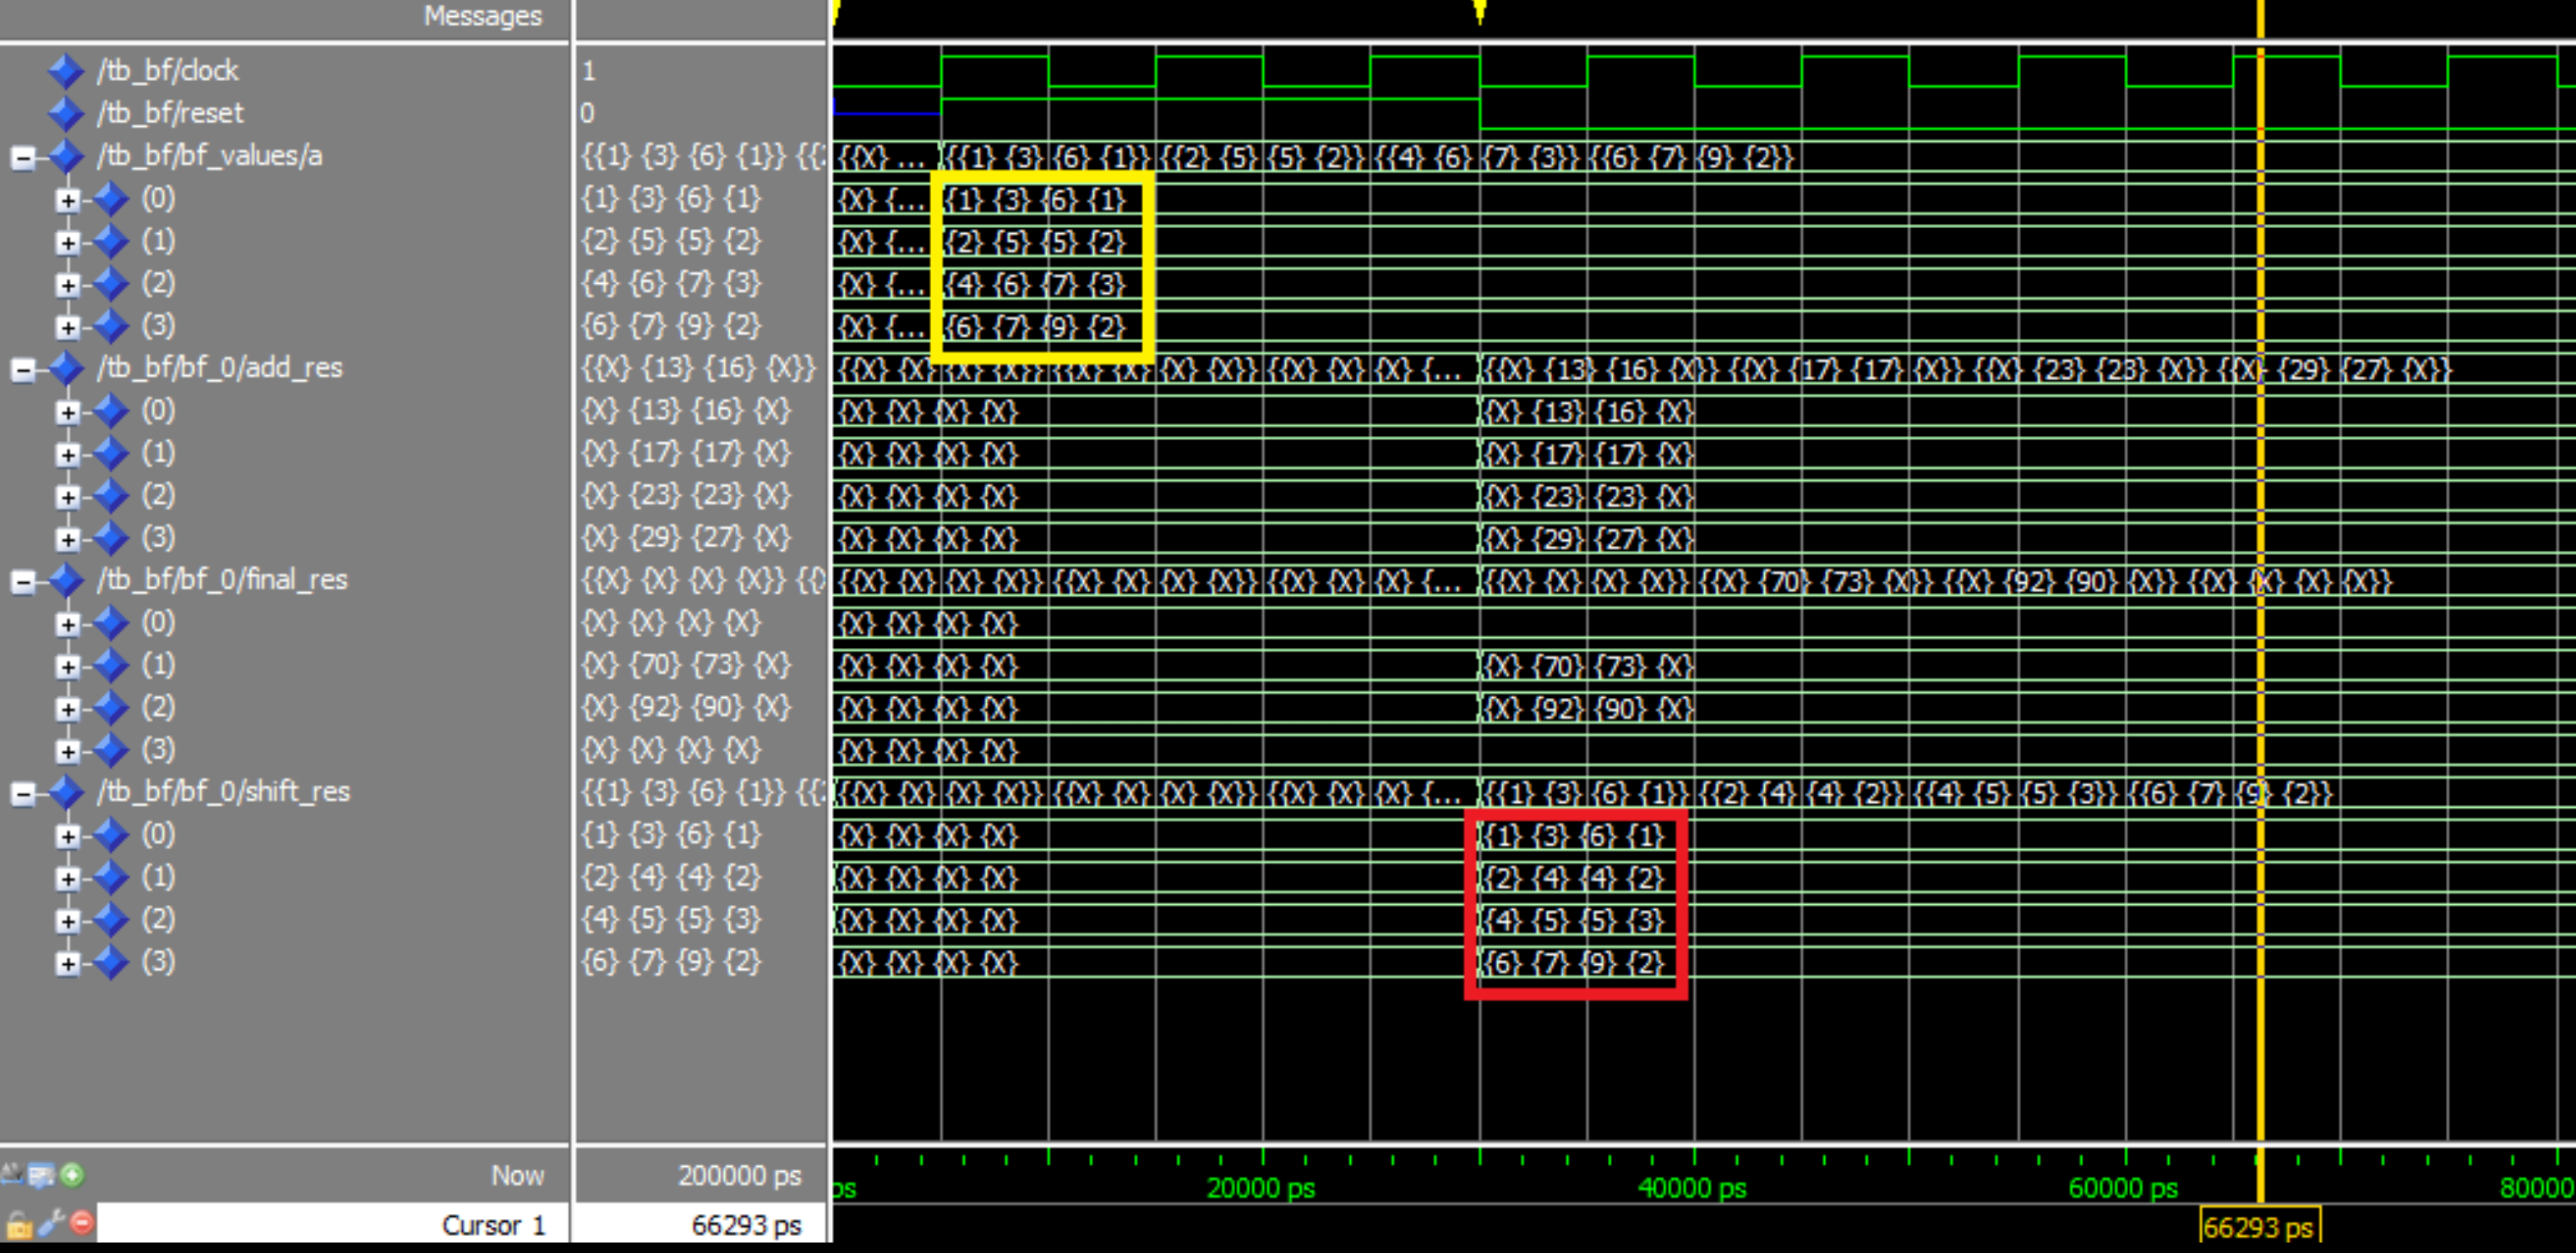
\includegraphics[width=\textwidth]{imm/bf/tb_bf.png}  
     	\caption{Binomial Filter-Results of the simulation type 1} 
     	\label{fig:tb_bf}
     \end{figure}
     
     At the beginning we have an input array that contains the values of the matrix   \begin{center}
     	$ \begin{bmatrix}
     	1 & 3 & 6 & 1\\
	     	2 & 5 & 5 & 2   	\\
	     	4&6 & 7 & 3\\
	     	6&7 & 9 & 2
	     	\end{bmatrix}$
	     	     \end{center}
	  The first step of this implementation is to do the partial weighted sum for three consecutive cell
	  \begin{center}
	  	$ S_{x,y}=cell_{x-1,y}+2\cdot cell_{x,y}+cell_{x+1,y}$\\
	  	$  \forall x\in [1,n-2] \quad\forall y\in[0,n-1]$
	  \end{center}
	   \begin{center}
	   	$ \begin{bmatrix}
	   	X\quad & 1+2\cdot3+6 \quad& 3+2\cdot6+1\quad & X\\
	   	X\quad & 2+2\cdot5+5 \quad& 5+2\cdot5+2\quad & X   	\\
	   	X\quad&4+2\cdot6+7 \quad& 6+2\cdot7+3\quad & X\\
	   	X\quad&6+2\cdot7+9 \quad& 7+2\cdot9+2\quad & X
	   	\end{bmatrix}$
	   \end{center}
	   which will lead us to the result
	   \begin{center}
	   	$ \begin{bmatrix}
	   		X & 13 & 16 & X\\
	   		X & 17 & 17 & X   	\\
	   		X&23 & 23 & X\\
	   		X&29 & 27 & X
	   	\end{bmatrix} $
	   \end{center}
	   which is the same shown in the simulation (fig \ref{fig:tb_bf}, \textit{add\_res} array).\\
	    Now we have to do the final sum
	   \begin{center}
	   	$ SUM_{x,y}=S_{x,y-1}+2\cdot S_{x,y}+S_{x,y+1}$\\
	   		$  \forall x\in [1,n-2] \quad\forall y\in [1,n-2] $
	   \end{center}
	   \bigskip
	  \begin{center}
	  	$ \begin{bmatrix}
	  	X & X & X & X\\
	  	X \quad& 13+2\cdot17+23\quad & 16+2\cdot17+23 \quad& X   	\\
	  	X\quad&17+2\cdot23+29 \quad& 17+2\cdot23+27 \quad& X\\
	  	X&X & X & X
	  	\end{bmatrix} = \begin{bmatrix}
	  	X & X & X & X\\
	  	X & 70 & 73 & X   	\\
	  	X&92 & 90 & X\\
	  	X&X & X & X
	  	\end{bmatrix}$
	  \end{center}
	  this matrix is the same we obtained in the simulation (fig \ref{fig:tb_bf}, \textit{final\_res} array).
	  The work is not over yet because we need to divide these sums by 16
	  \begin{center}
	  	$ \begin{bmatrix}
	  	X & X & X & X\\
	  	X & \frac{70}{16} & \frac{73}{16} & X   	\\
	  	X&\frac{92}{16}  & \frac{90}{16}  & X\\
	  	X&X & X & X
	  \end{bmatrix}=\begin{bmatrix}
	  X & X & X & X\\
	  X & 4.375 & 4.5625 & X   	\\
	  X&5.75  & 5.625  & X\\
	  X&X & X & X
	  \end{bmatrix}$
	  \end{center}
	  Since the values of the pixel are integer, we can round the matrix as\begin{center}
	  	$ 
	  \begin{bmatrix}
	  	X & X & X & X\\
	  	X & 4 & 4 & X   	\\
	  	X&5  & 5  & X\\
	  	X&X & X & X
	  \end{bmatrix}$
	  \end{center}
	  so the final result is \begin{center}
	  	$ 
	  	\begin{bmatrix}
	  	1 & 3 & 6 & 1\\
	  	2 & 4 & 4 & 2   	\\
	  4&5  & 5  & 3\\
	  	6&7 & 9 & 2
	  	\end{bmatrix}$
	  \end{center}
	  which is the same as shown in the simulation (fig \ref{fig:tb_bf}, \textit{shifft\_res} array).
	  \subsection{Simulation type 2}
	
	  The simulation shown in this work is referred to the hardware implementation descrived in the subsection \ref{h2} where also the final values of the matrix's border are computed using the binomial filter criteria.
	  In this testbench, we have a matrix 4x4 (fig.\ref{fig:tb_bf} highlighted in yellow, and the output highlighted in red).
	  
	  
	  \begin{figure}[h!]
	  	\centering	
	  	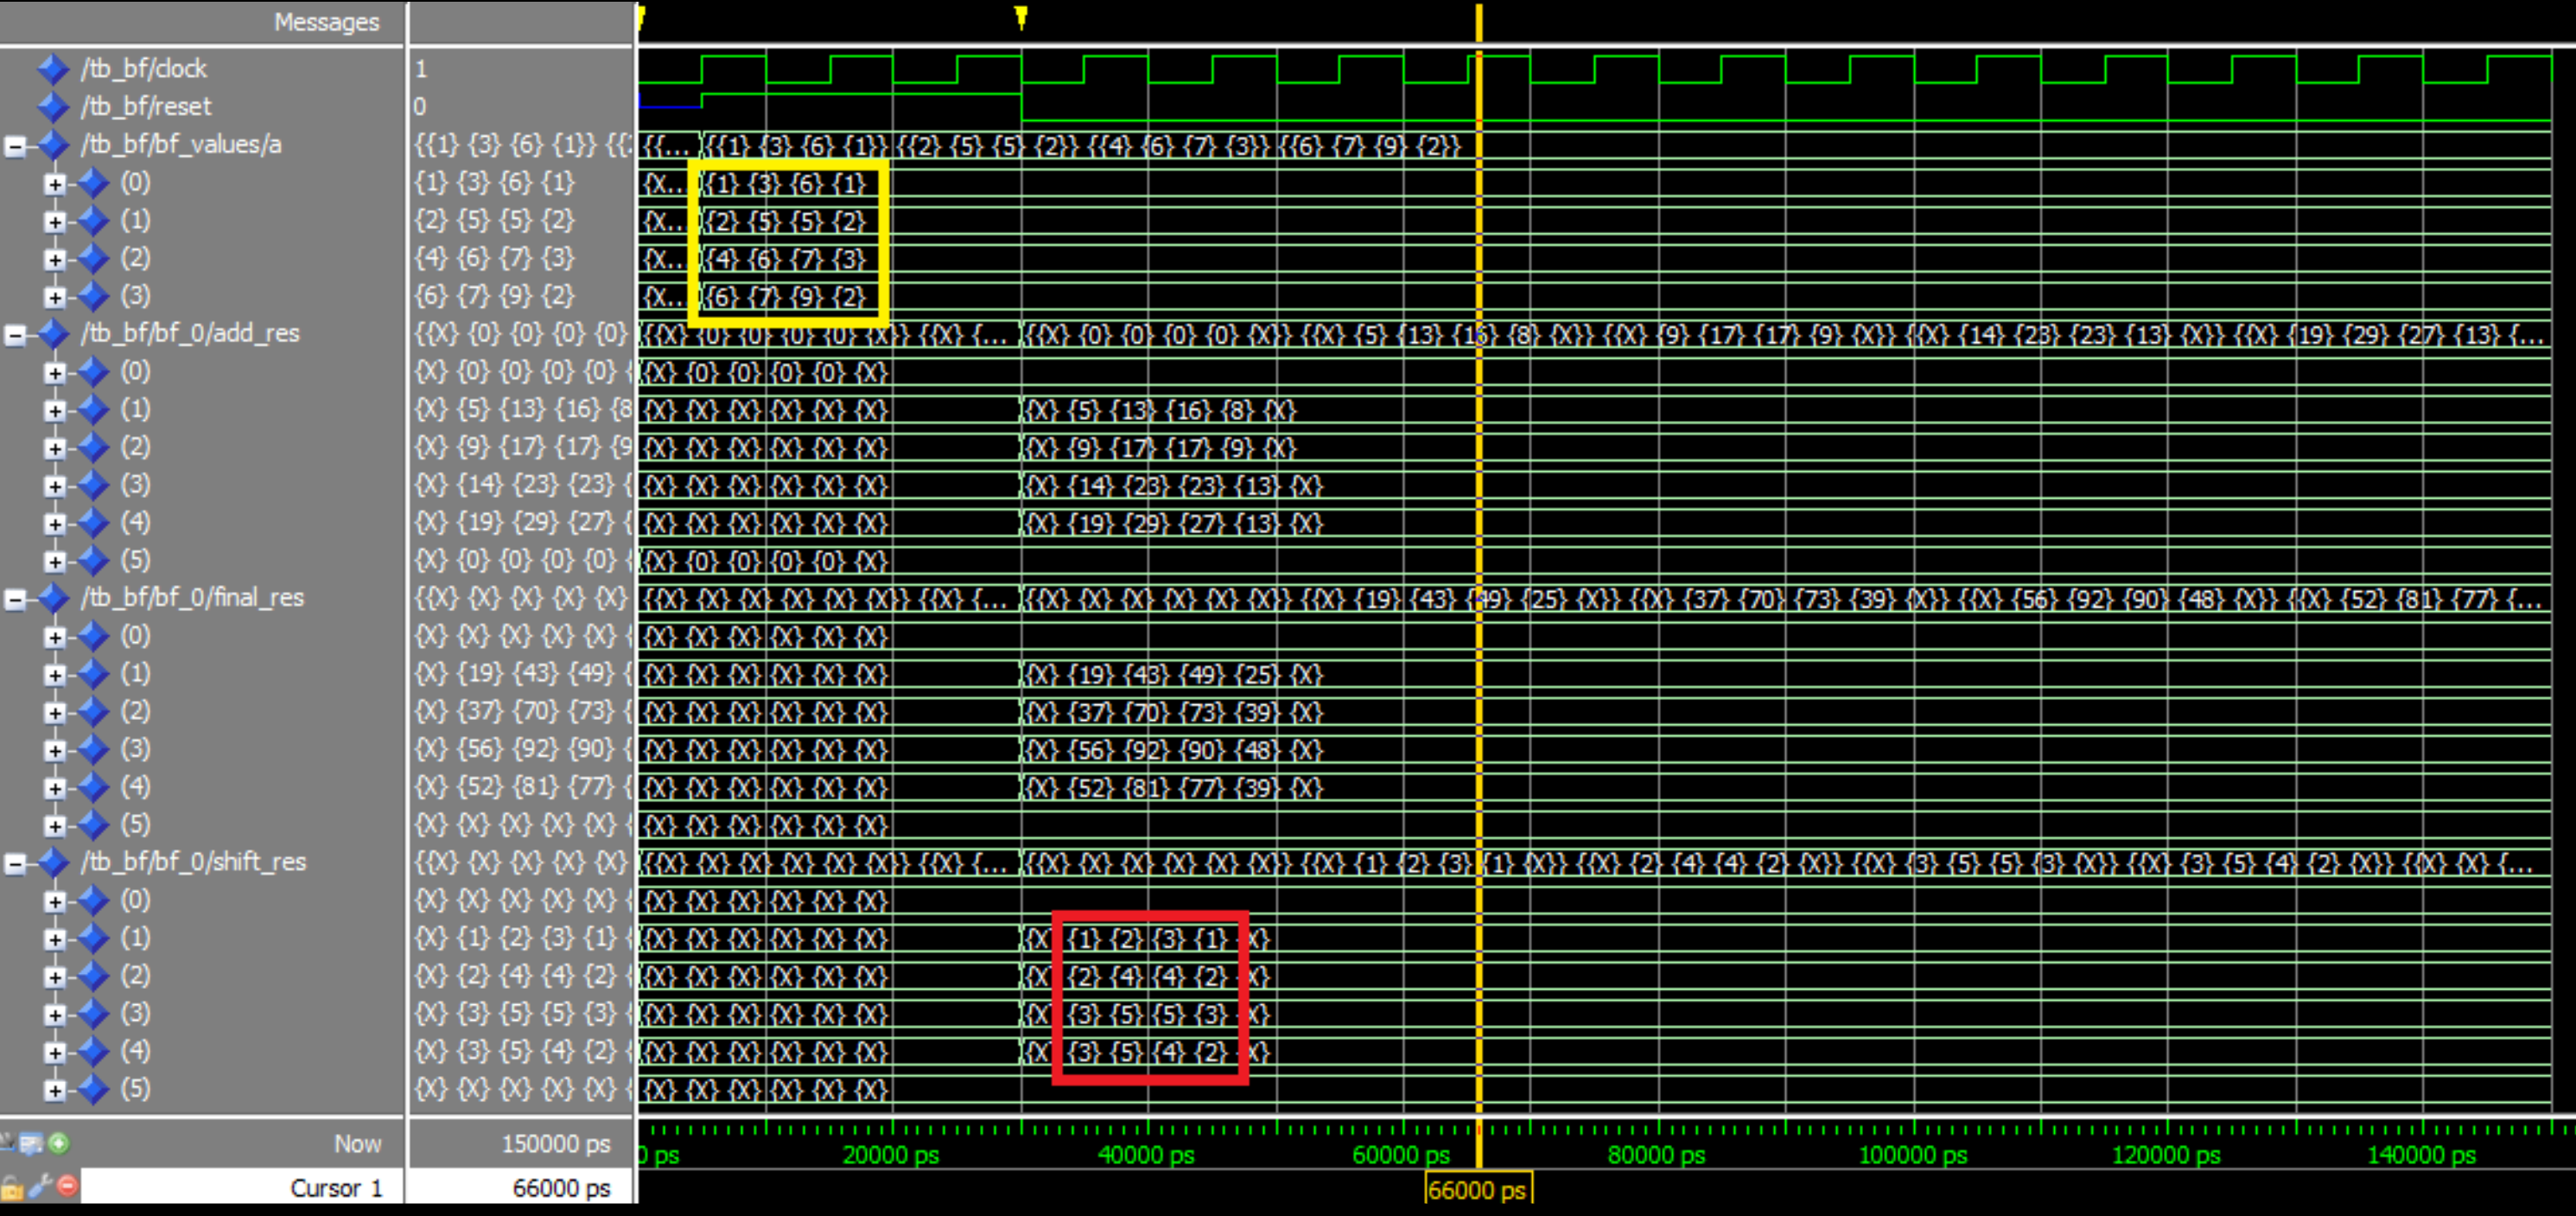
\includegraphics[width=\textwidth]{imm/bf/bfwavev2.png}  
	  	\caption{Binomial Filter-Results of the simulation type 2} 
	  	\label{fig:tb_bf2}
	  	\end{figure}
	At the beginning we have an input array that contains the values of the matrix   \begin{center}
		$ \begin{bmatrix}
		1 & 3 & 6 & 1\\
		2 & 5 & 5 & 2   	\\
		4&6 & 7 & 3\\
		6&7 & 9 & 2
		\end{bmatrix}$
	\end{center}
	For this implementation, we will perform the binomial filter for the matrix that has a border of  $ '0' $ and in the center the input matrix.
	 \begin{center}
	 	$ \begin{bmatrix}
	 	0&0 &0  &0  & 0&0\\
	 	0&1 & 3 & 6 & 1&0\\
	 	0&2 & 5 & 5 & 2  &0 	\\
	 0&	4&6 & 7 & 3&0\\
	 0&	6&7 & 9 & 2&0\\
	 	0&0 &0  &0  & 0&0
	 	\end{bmatrix}$
	 	 \end{center}
Now we perform the same steps described in section \ref{sim1}.	
We do the partial weighted sum for three consecutive cell
\begin{center}
	$ S_{x,y}=cell_{x-1,y}+2\cdot cell_{x,y}+cell_{x+1,y}$\\
	$  \forall x\in [1,n-2] \quad\forall y\in[0,n-1]$
\end{center} 	 
	\begin{center}
		$ \begin{bmatrix}
		X&0&0&0&0&X\\
		X\quad&2\cdot1+3\quad & 1+2\cdot3+6 \quad& 3+2\cdot6+1\quad & 6+2\cdot1\quad&X\\
		X\quad&2\cdot2+5\quad & 2+2\cdot5+5 \quad& 5+2\cdot5+2\quad & 5+2\cdot2  \quad&X 	\\
		X\quad&2\cdot4+6\quad&4+2\cdot6+7 \quad& 6+2\cdot7+3\quad & 7+2\cdot3\quad&X\\
		X\quad&2\cdot6+7\quad&6+2\cdot7+9 \quad& 7+2\cdot9+2\quad & 9+2\cdot2\quad&X\\
		X&0&0&0&0&X
		\end{bmatrix}$
	\end{center}
	which will lead us to the result
	\begin{center}
		$ \begin{bmatrix}
		X&0&0&0&0&X\\
		X\quad&5\quad & 13 \quad& 16\quad & 8\quad&X\\
		X\quad&9\quad &17 \quad& 17\quad & 9  \quad&X 	\\
		X\quad&14\quad&23 \quad&23\quad & 13\quad&X\\
		X\quad&19\quad&29 \quad& 27\quad & 13\quad&X\\
		X&0&0&0&0&X
		\end{bmatrix}$
	\end{center}
	which is the same shown in the simulation (fig \ref{fig:tb_bf2}, \textit{add\_res} array).\\ 	 
	  	Now we have to do the final sum
	  	\begin{center}
	  		$ SUM_{x,y}=S_{x,y-1}+2\cdot S_{x,y}+S_{x,y+1}$\\
	  		$  \forall x\in [1,n-2] \quad\forall y\in [1,n-2] $
	  	\end{center}
	  	\bigskip
	  	\begin{center}
	  		$ \begin{bmatrix}
	  		X & X & X & X &X&X\\
	  		X\quad & 2\cdot5+9\quad& 2\cdot13+17\quad&2\cdot16+17\quad&2\cdot8+9\quad&X\\
	  		X \quad&5+2\cdot9+17\quad& 13+2\cdot17+23\quad & 16+2\cdot17+23 \quad& 8+2\cdot9+13\quad&X   	\\
	  		X\quad&9+2\cdot14+19\quad&17+2\cdot23+29 \quad& 17+2\cdot23+27 \quad& 9+2\cdot13+13\quad&X\\
	  		X\quad & 14+2\cdot19\quad& 23+2\cdot29\quad&23+2\cdot27\quad&13+2\cdot13\quad&X\\
	  		X&X & X & X &X&X
	  		\end{bmatrix} = $
	  		\bigskip$=\begin{bmatrix}
	  	X & X & X & X &X&X\\
	  	x & 19 & 43 & 49 & 25 & X\\
	  	X & 37 &70 & 73 & 39 & X   	\\
	  		X&56 & 92 & 90 & 48& X\\
	  		X&52&81&77&39&X\\
	  		X & X & X & X &X&X
	  		\end{bmatrix}$
	  	\end{center}
	  	this matrix is the same we obtained in the simulation (fig \ref{fig:tb_bf2}, \textit{final\_res} array).
	  	The work is not over yet because we need to divide these sums by 16\\
	  	\begin{center}
	  	$	\begin{bmatrix}
  			X & X & X & X &X&X\\
  			X & \frac{19}{16} & \frac{43}{16} & \frac{49}{16} & \frac{25}{16} & X\\
  			X & \frac{37}{16} &\frac{70}{16} & \frac{73}{16} & \frac{39}{16} & X   	\\
  			X&\frac{56}{16} & \frac{92}{16} & \frac{90 }{16}& \frac{48}{16}& X\\
  			X&\frac{52}{16}&\frac{81}{16}&\frac{77}{16}&\frac{39}{16}&X\\
  			X & X & X & X &X&X
	  		\end{bmatrix}=	\begin{bmatrix}
	  		X & X & X & X &X&X\\
	  		X & 1.1875 & 2.6875 & 3.0625 & 1.5625 & X\\
	  		X & 2.3125 &4.375 & 4.5625 & 2.4375 & X   	\\
	  		X&3.5 & 5.75 & 5.625& 3& X\\
	  		X&3.25&5.0625&4.8125&2.4375&X\\
	  		X & X & X & X &X&X
	  		\end{bmatrix}$
	  	\end{center}\bigskip
	  	Since the values of the pixel are integer, we can round the matrix as\\
	  	\begin{center}
	  		$	\begin{bmatrix}
	  		X & X & X & X &X&X\\
	  		X & 1 & 2 & 3 & 1 & X\\
	  		X & 2 &4 & 4 & 2 & X   	\\
	  		X&3 & 5 & 5& 3& X\\
	  		X&3&5&4&2&X\\
	  		X & X & X & X &X&X
	  		\end{bmatrix}$
	  		\end{center}
	  	
	  \section{Comparison}
	  \subsubsection{Logic-In-Memory implementation}
	  The architecture of the Logic-In-memory was already explained in the subsection \ref{sssec:1}.
	  The pseudocode for the LIM is
	  \begin{enumerate}
	  	\item Each cell reads its own value;
	  	\item Reads all neighbouring cells data (8 different values); 
	  	\item Sums all values and divides them by 16;
	  	\item Writes the final result in its own memory;
	  \end{enumerate}
	 The main advantage of the LIM architecture is the parallelism: the presence of many cells that can work autonomously greatly increases the speed of the computation of algorithms that can be executed in parallel.
	 It has been calculated that the total duration for the computation is equal to: 
	 \begin{itemize}
	 	\item N clock cycles to write the data;
	 	\item 28 clock cycles to compute the algorithm;
	 	\item 2N+1 clock cycles to read the data through a remote read. Therefore,
	 \end{itemize}   \begin{center}
	 	 $ t = N + 28 + 2N +1=3N + 29 $
	\end{center}
	
	 \begin{center}
	 	\begin{tabular}{ | p{1.7cm} | c | c |}
	 		
	 		\hline
	 		\label{table:bf_tab} & LIM & This work \\
	 		\hline
	 		Area & $ N\cdotp N $ cells  &  $ N\cdotp (N-2)+(N-2)\cdotp (N-2)$ adders \\
	 		\hline
	 		Time & $ 3N + 29 $ cycles
	 		&
	 		 time for 4 adders   \\
	 		\hline
	 		
	 	\end{tabular}
	 \end{center}
	As for this work by looking to the section \ref{bfh}, we know that the time required is the time for 4 adder in sequence, this because 2 adder are required for doing the weighted sum of 3 consecutive cells, and the other 2 for doing the weighted sum of the 9 cells


%\chapter{Digital Filter FIR}
A digital filter is a system performing a certain function on an input stream $ X[n] $ (samples are received at constant rate) and generating an output stream called $ Y[n] $. 
In general it's possible to have multiple input streams and multiple output streams (for example in a parallel architecture this allows to speed up the filter).
\section{Digital filters properties}
Filters are systems characterized by the following properties \cite{fir1}:
\begin{enumerate}
	\item \textbf{Linearity}: it is possible to represent the output as an overlapping of the input pulses. Let $\delta[n-k]$ be the input signal and $ h_{k}[n] $ the filter response, using overlapping property, assuming that the input is a sum of pulses: 
	\begin{center}
		$ x[n]=\sum\limits_{k}^{} (x[n]\cdot \delta[n-k]) $
		\end{center}
		so the output is: $ h_{k}[n] =F(\delta[n-k])$ (F is the filter funtion), so applying linearity: 
			\begin{center}
				$ F(x[n])=F(\sum\limits_{k}^{ } (x[n]\cdot \delta[n-k])) $\\
			\end{center}
			\begin{center}
				$ y[n]=\sum\limits_{k}^{ } x[n]\cdot h_{k}[n] $
			\end{center}
    It means that if the input is a weighted sum of pulses, also the output will have the same form.
    \item  \textbf{Time invariance}: the shape of the answer $ h_{k} $ is not dependent on the selected time $ k $. So applying the same input signal at different time (i.e. different $ k $), the filter response will be always the same, just time-shifted. Therefore:
    
    \begin{center}
    	$ h_{k}[n] = h[n-k]  $
    \end{center}
    The expression for the output found before can be rewritten as:
    \begin{center}
    	$ y[n]=\sum\limits_{k}^{ } x[n]\cdot h_{k}[n]= \sum\limits_{k}^{ } x[n]\cdot h[n-k]=x[n]\ast h[n]$
    \end{center}
    where it has been used the definition of convolution product.
    \item \textbf{Stability}: we expect to have at the output a stable stream of samples whose values do not diverge. This is true if a sufficient numbers of bit has been employed for representing the samples. Assuming that the system is BIBO (bounded input bounded output), the following condition should be satisfied: 
    \begin{center}
    	$ S=\sum\limits_{k}^{ } |h[n]| < \infty $
    \end{center}
    \item \textbf{Causality}: if we apply an input at time $ k $,
     we expect that the output doesn't come before time $ k $.
     Assuming that $ x[n] = 0  $ for $ n < 0 $, then $ y[n] = 0 $ for $ k < 0 $: this property is true only if $  h[n] = 0 $ for $ n < 0 $ 
    
\end{enumerate}

\section{Hardware Implementation}
An FIR filter can be easily implemented using just three digital hardware elements, a unit delay (D Flip Flop), a multiplier, and an adder. The unit delay simply updates its output once per sample period, using the value of the input as its new output value. In the convolution sum,

\begin{center}
	$ 	 y[n]=\sum\limits_{k}^{ } x[n]\cdot h[n-k] =\sum\limits_{k}^{ } x[n-k]\cdot h[n]$
\end{center}
notice that at each $ n $ we need access to $ x(n)$, $x(n - 1)$, $x(n - 2)$, $\cdots$, $x(n - k) $. We can maintain this set of values by cascading a set of D Flip Flops to form a delay line, as shown in Fig. \ref{fig:fir1}
\begin{figure}[h!]
	\centering
	
\includegraphics[width=0.9\textwidth]{imm/fir/fir1.png}  
	\caption{Cascading D Flip Flops} 
	\label{fig:fir1}
\end{figure}

For each of the previous $ k $ inputs, we have to scale them by $ h(0) $, $ h(1) $, $ \cdots $, $ h(k) $. To obtain these values, we simply put a multiplier as shown in the following picture (Fig. \ref{fig:fir2}).
To obtain the final result, we have to sum all the results of these multiplications.
\begin{figure}[h!]
	\centering
	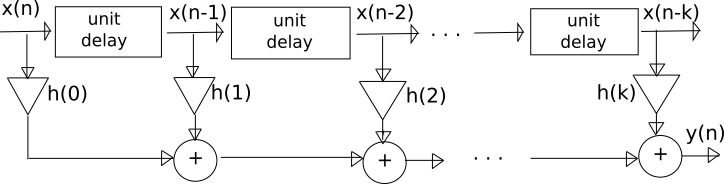
\includegraphics[width=0.9\textwidth]{imm/fir/fir2.png}  
	\caption{FIR hardware implementation} 
	\label{fig:fir2}
\end{figure}
\section{Simulation}
The simulation shown in this work has 6 constants (fig. \ref{fig:fir_sim}, \textit{fir\_constants\_value} section)
\begin{center}
	$ h_{0}=12$\\
	$h_{1}=10$\\
	$h_{2}= 8$\\
	$h_{3}= 6$\\
	$h_{4}= 4$\\
	$h_{5}= 2$\\
\end{center}
and it will take into account the last 6 inputs.\\
\begin{figure}[h!]
	\centering
	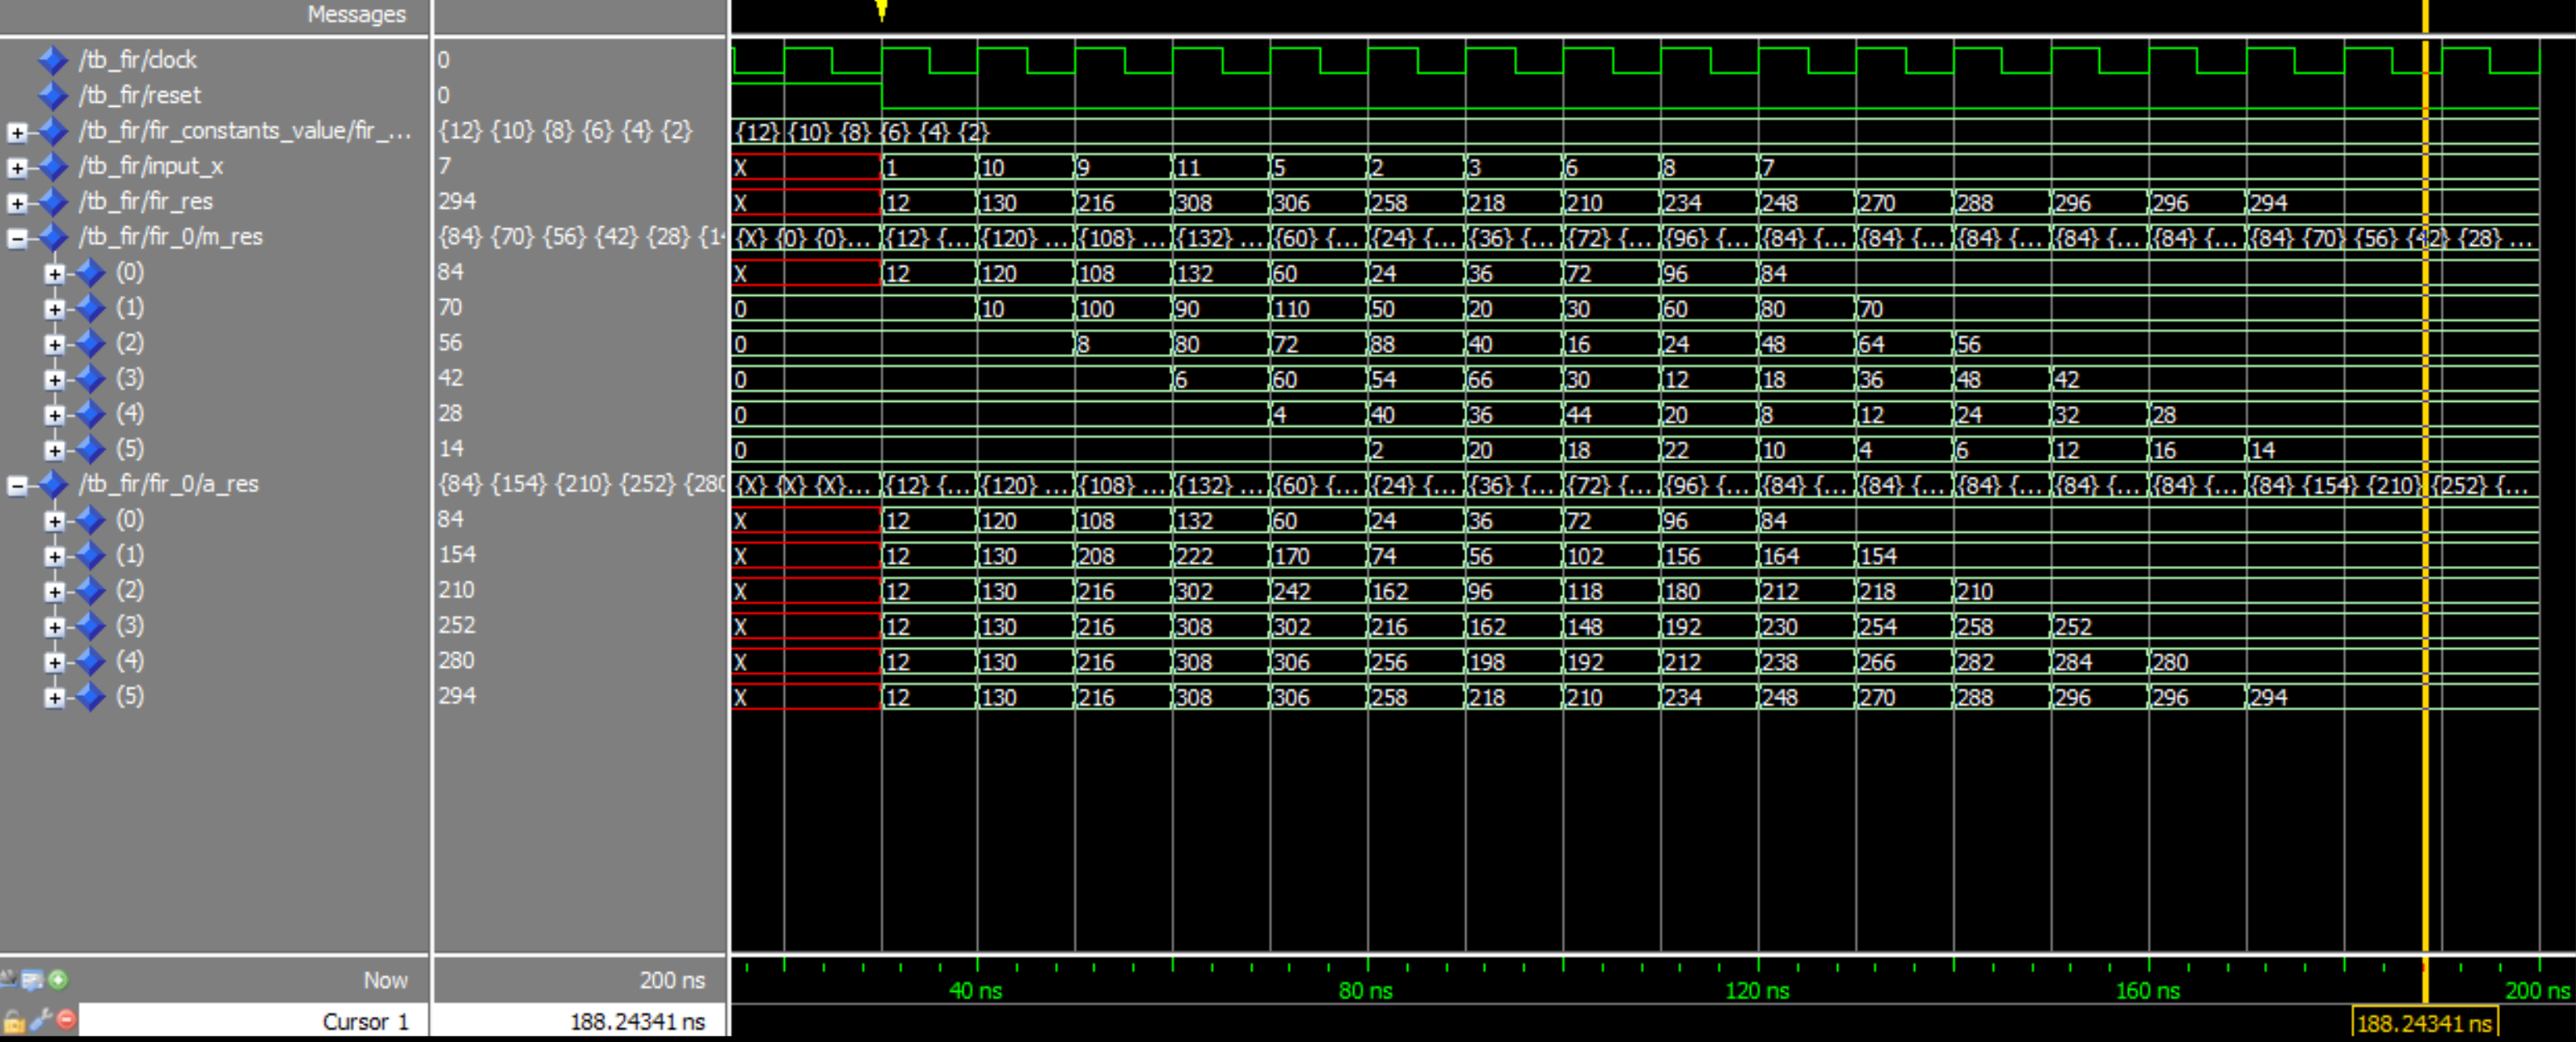
\includegraphics[width=\textwidth]{imm/fir/fir_sim.png}  
	\caption{FIR's simulation} 
	\label{fig:fir_sim}
\end{figure}
When we start sampling after the reset, we set all the previous inputs to $ '0' $, therefore the output will be simply $ y[n]=x[n]\cdot h_{0} $.\\
In fact in the simulation, as soon as the reset was set low, we see the output (fig. \ref{fig:fir_sim},\textit{fir\_res} signal) to be\begin{center}
	 $ y[n]=x[n]\cdot h_{0}=1\cdot12=12 $.
\end{center}
In the next cycle we get \begin{center}
	$ y[n]=x[n]\cdot h_{0}+x[n-1]\cdot h_{1}=10\cdot12+1\cdot 10=130 $.
\end{center}
For the next clock cycles we repeat the same procedure.\\
In the end, when the input has not changed for more than 6 clock cycles, we can see the result to be 
\begin{center}
	$ y[n]=\sum\limits_{k=0}^{6 } x[n-k]\cdot h[k]=7\sum\limits_{k=0}^{6 }=7\cdot42=294$
\end{center}
\clearpage
\newpage
\section{Characteristics of Filter FIR}
\vspace{10pt}
{\large \textbf{PROCESSING ELEMENTS}}\vspace{10pt}\\
\begin{tabular}{ p{0.2cm} p{14.5cm}}
	
	&\textbf{1- Which kind of Processing element?}\\
	&	Adder, multiplier, registers\vspace{7pt}\\
	&	\textbf{2- Functionality}\\
	&	Addition, multiplications, storing.\vspace{7pt}\\
	&	\textbf{3- Complexity}\\
	&	\begin{tabular}{ p{0.2cm} p{1.2cm}  p{13cm}}
		
		& Area: &$ N-1 $ adders\\
		& & $N-1$ registers\\
		& & $N$ multipliers\\
		 & Time: &Time for one registers, one multiplication and  $N-1 $ additions \vspace{3pt}\\
	
		
	\end{tabular}\vspace{7pt}\\
	&	\textbf{4- Parallelism}\\
	&	Registers and multiplications can work in parallel, The chain made of adder not (fig. \ref{fig:fir2}).\vspace{7pt}\\
	&	\textbf{5-Reconfigurability}\\
	&	No\vspace{7pt}\\
	&	\textbf{6- Programmability}\\
	&	No\vspace{7pt}\\
	&	\textbf{7- Need a dedicated memory?}\\
	&	It needs some memory to store the previous $N-1$ input values.\\
	&It is possible also to store the $N$ constants\vspace{7pt}\\
	&\textbf{8- Relationship with I/O}\\
	&	INPUT: values of the input and values of the constatnts.\\
	&	OUTPUT: result of the filter FIR algorithm\end{tabular}\vspace{74pt}\\
\newpage{\large \textbf{\qquad }}\vspace{10pt}\\
{\large \textbf{MEMORY ELEMENTS}}\vspace{10pt}\\\begin{tabular}{ p{0.2cm} p{14.5cm}}
	&\textbf{1- Need a clever memory LIM?}\\
	&	No, but can be implemented\vspace{7pt}\\
	&\textbf{2- Is there a data search algorithm?}\\
	&	No\vspace{7pt}\\
	&\textbf{	3-Interface mechanism with other PE or memories}\\
	&	Communication required between local elements\vspace{7pt}\\
	&	\textbf{4- Access mechanism}\\
	&	(No memory for this implementation)\vspace{7pt}\\
	&	\textbf{5- Hierarchization} \\
	&	(No memory for this implementation)\vspace{7pt}\\
	&\textbf{	6- Cache coherency} \\
	&	(No memory for this implementation)\vspace{7pt}\\
	&\textbf{	7- Is it a a transactional memory?}\\
	&	(No memory for this implementation)\vspace{7pt}\\
	&\textbf{	8- Are there virtualization (paging) mechanisms?}\\
	&	(No memory for this implementation)\end{tabular}\vspace{14pt}\\
\vspace{10pt}\\
{\large\textbf{ENCODING INFORMATION}}\vspace{10pt}\\
\begin{tabular}{ p{0.2cm} p{14.5cm}}
	&\textbf{1-Which encoding is used?}\\
	&Binary encoding
\end{tabular}
\newpage{\large\textbf{ }}\vspace{10pt}\\
{\large\textbf{CONNECTIONS}}\vspace{10pt}\\\begin{tabular}{ p{0.2cm} p{14.5cm}}
	&\textbf{1-Packet Exchange Protocol}\\
	&Directly\vspace{7pt}\\
	&\textbf{2-Timing (asynchronou/synchronous)}\\
	&Synchronous\vspace{7pt}\\
	&\textbf{3-Are there multiple instances? }\\
	&Yes\vspace{7pt}\\
	&\textbf{4-Heterogeneity (Local/Distant I/O Connections)}\\
	&Heterogeneous. Each elements is connected to the previous and following elementss. (No connections between distant elements)\vspace{7pt}\\
	&\textbf{5-Are there any buffers?}\\
	&There are some registers.
\end{tabular}\vspace{14pt}\\

%\chapter{Transport equation problem}
Fluid dynamics and transport phenomena, such as heat and mass transfer, play a vitally important role in human life.\\
Gases and liquids surround us, flow inside our bodies, and have a profound influence on the environment in which we live.\\
 Fluid flows produce winds, rains, floods, and hurricanes.\\ Convection and diffusion are responsible for temperature fluctuations and transport of pollutants in air, water or soil.\\
The ability to understand, predict, and control transport phenomena is essential for many industrial applications,such as aerodynamic shape design, oil recovery from an underground reservoir, or multiphase/multicomponent flows in furnaces, heat exchangers, and chemical reactors. \\Heating, air conditioning, and weather forecast have become an integral part of our everyday life. \\
The traditional approach to investigation of a physical process is based on observations, experiments, and measurements. The amount of information that can be obtained in this way is usually very limited and subject to measurement errors.\\
Moreover, experiments are only possible when a small-scale model or the actual equipment has already been built. An experimental investigation may be very time consuming, dangerous, prohibitively expensive, or impossible for another reason.
Alternatively, an analytical or computational study can be performed on the basis of a suitable mathematical model. As a rule, such a model consists of several differential and/or algebraic equations which make it possible to predict how the quantities of interest evolve and interact with one another.\\
\bigskip

The equations and the functionality used in this work, are the same described in the work of a student for the Logic-In-Memory. \\
The transport equation is a partial differential equation that describes the distribution of heat (or variation in temperature) in a given region over time.
\begin{equation}
	\dfrac{\partial}{\partial x} + \dfrac{\partial}{\partial y} = -\dfrac{\partial}{\partial t}
\end{equation}
Temperature values are calculated over a grid and initialized with a gaussian distribution. The points of the grid represent the local indexes (ix, iy) of the matrix that contains the temperature values. The domain is shown in orange in the picture below. Boundaries are represented in white. Data are evolved along Y=X direction, i.e. towards the up-right corner of the coordinate system.

\begin{figure}[h!]
	\centering
	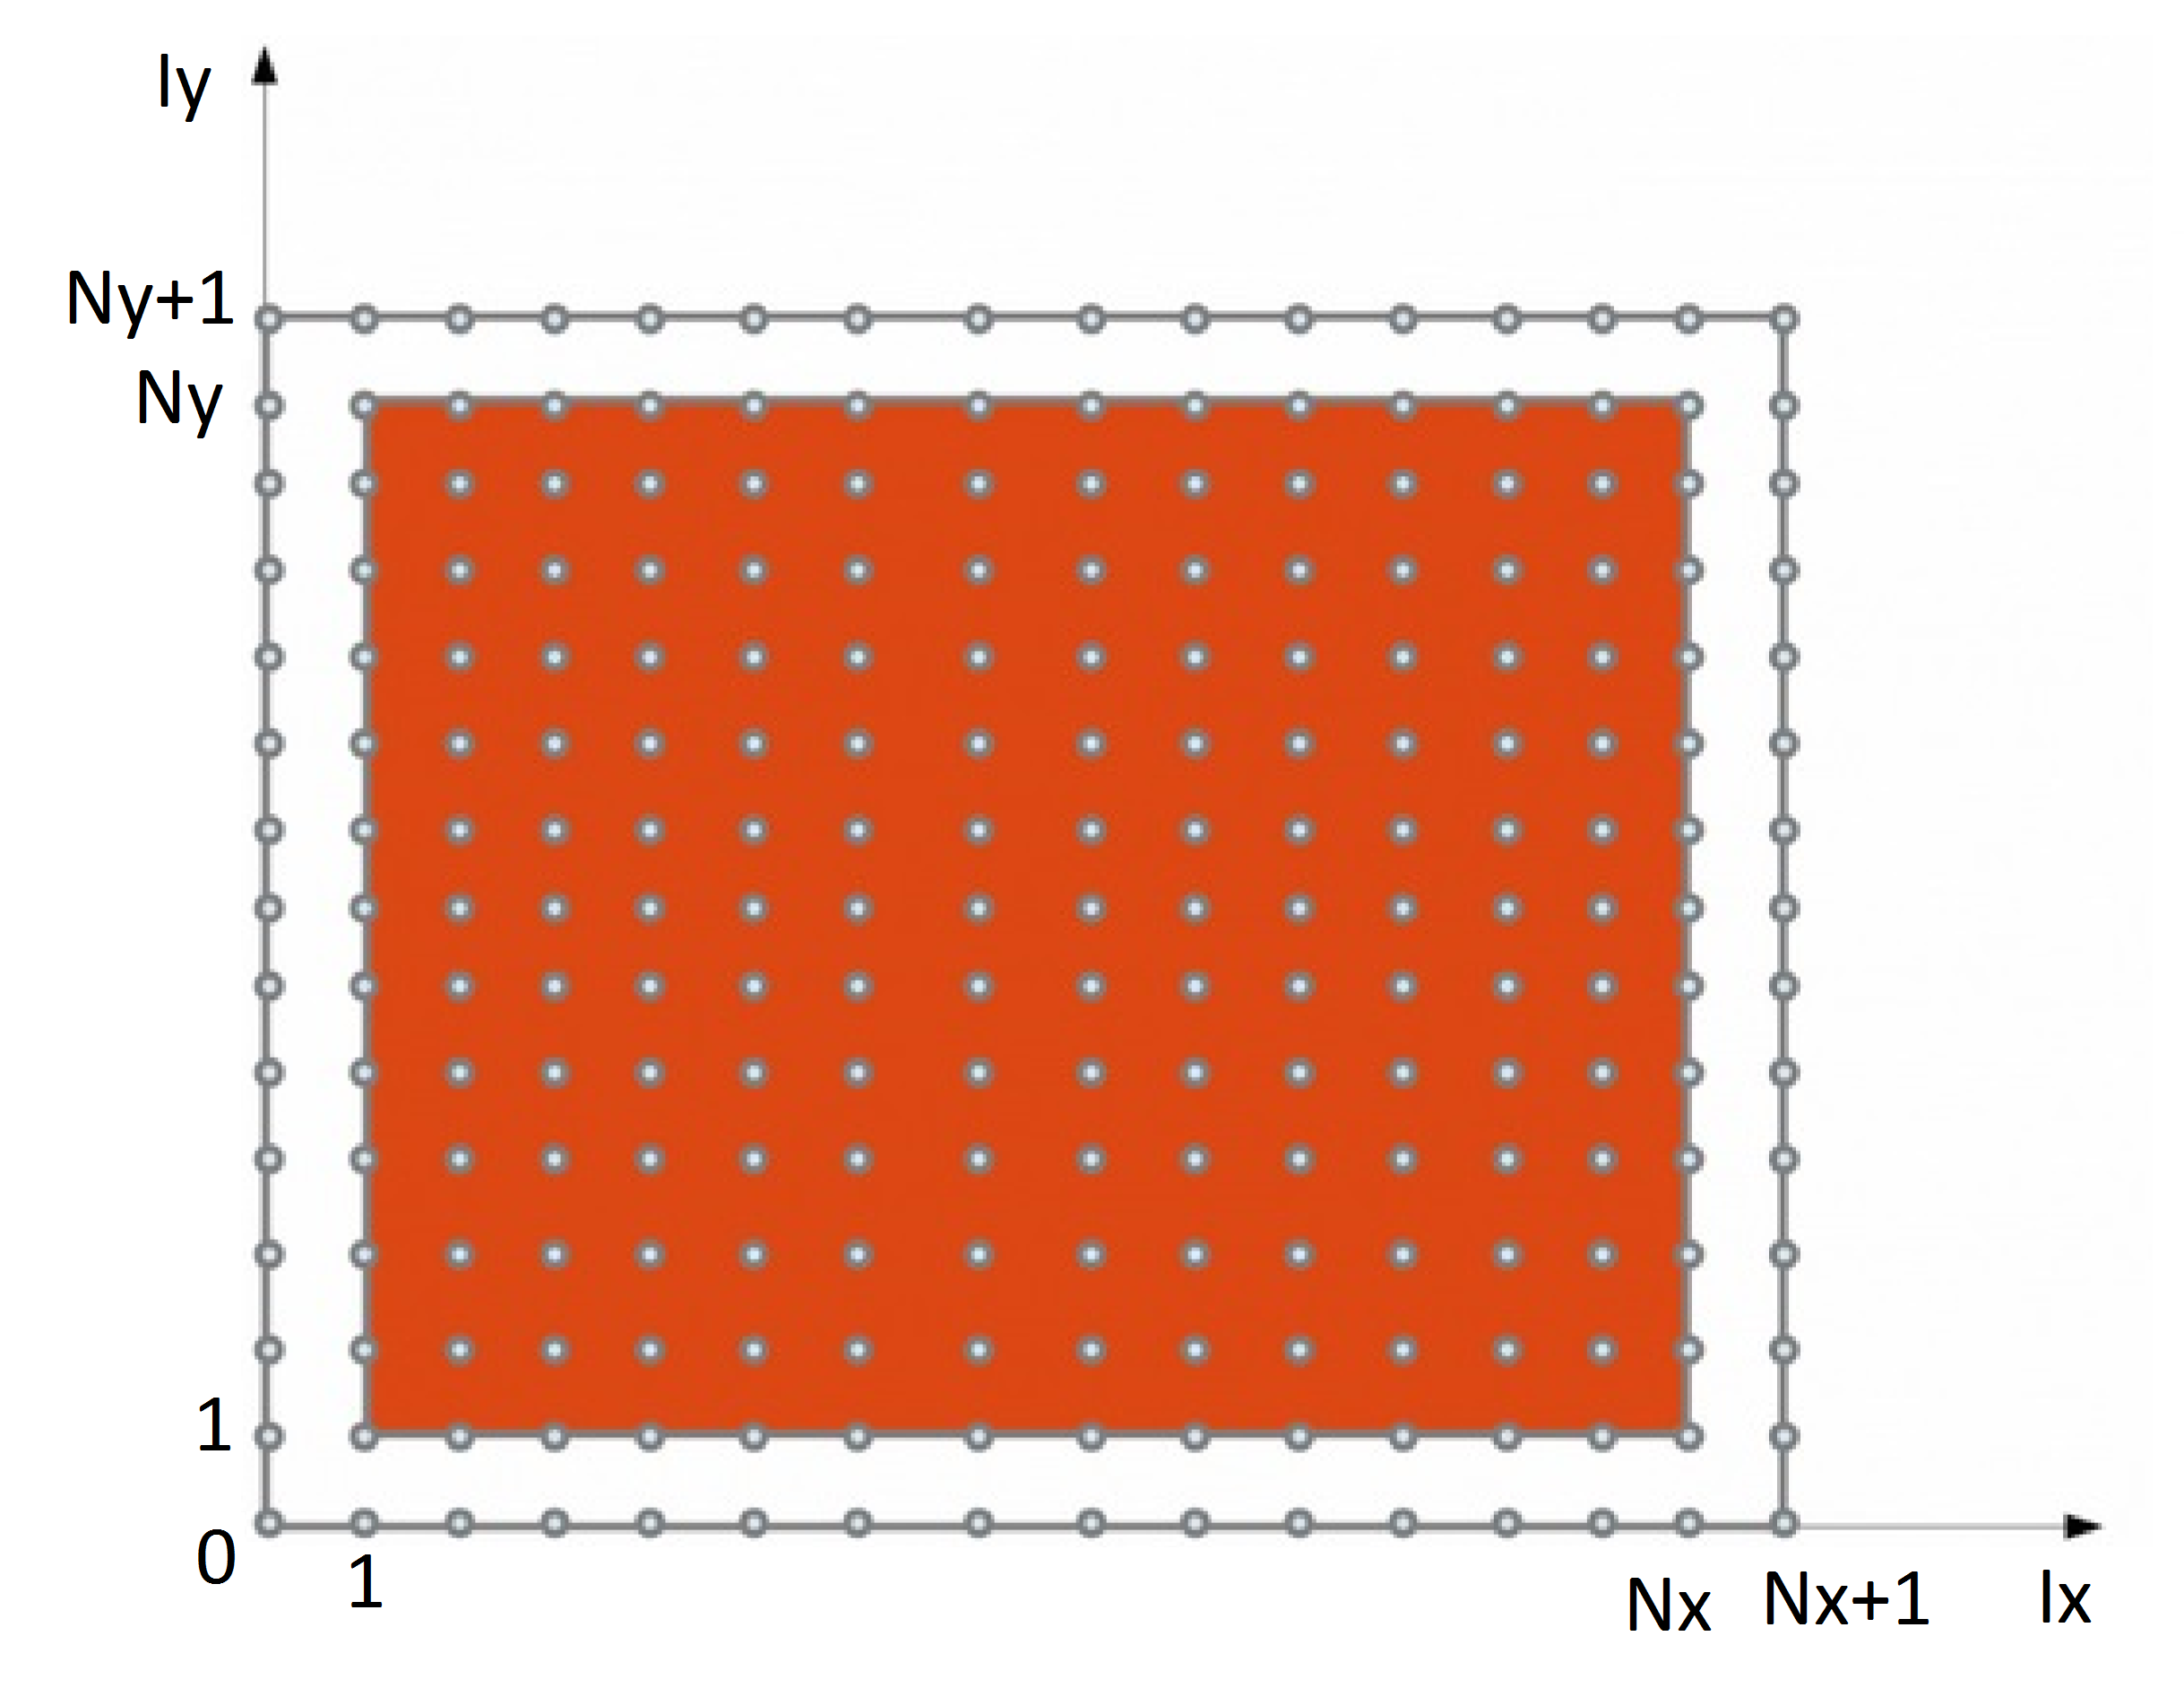
\includegraphics[width=0.8\textwidth]{imm/tep/tep0.png}  
	\caption{Grid for the Transport equation Problem} 
	\label{tep0}
\end{figure}
\bigskip
Each dot of the grid represents a cell. All the cells inside the orange rectangle have to calculate the new value of temperature and the cells at the boundary have to copy the calculated value from the cells at the border of the orange rectangle. Each cell works autonomously performing these calculations: 
\begin{equation}
	temp = t_{0}-\alpha[t(i+1,j)-t(i-1,j)+t(i,j + 1)-t(i,j-1)] 
\end{equation}
As shown below, each cell reads the values of temperature of the adjacent cells to compute the equation illustrated above:
\begin{figure}[h!]
	\centering
	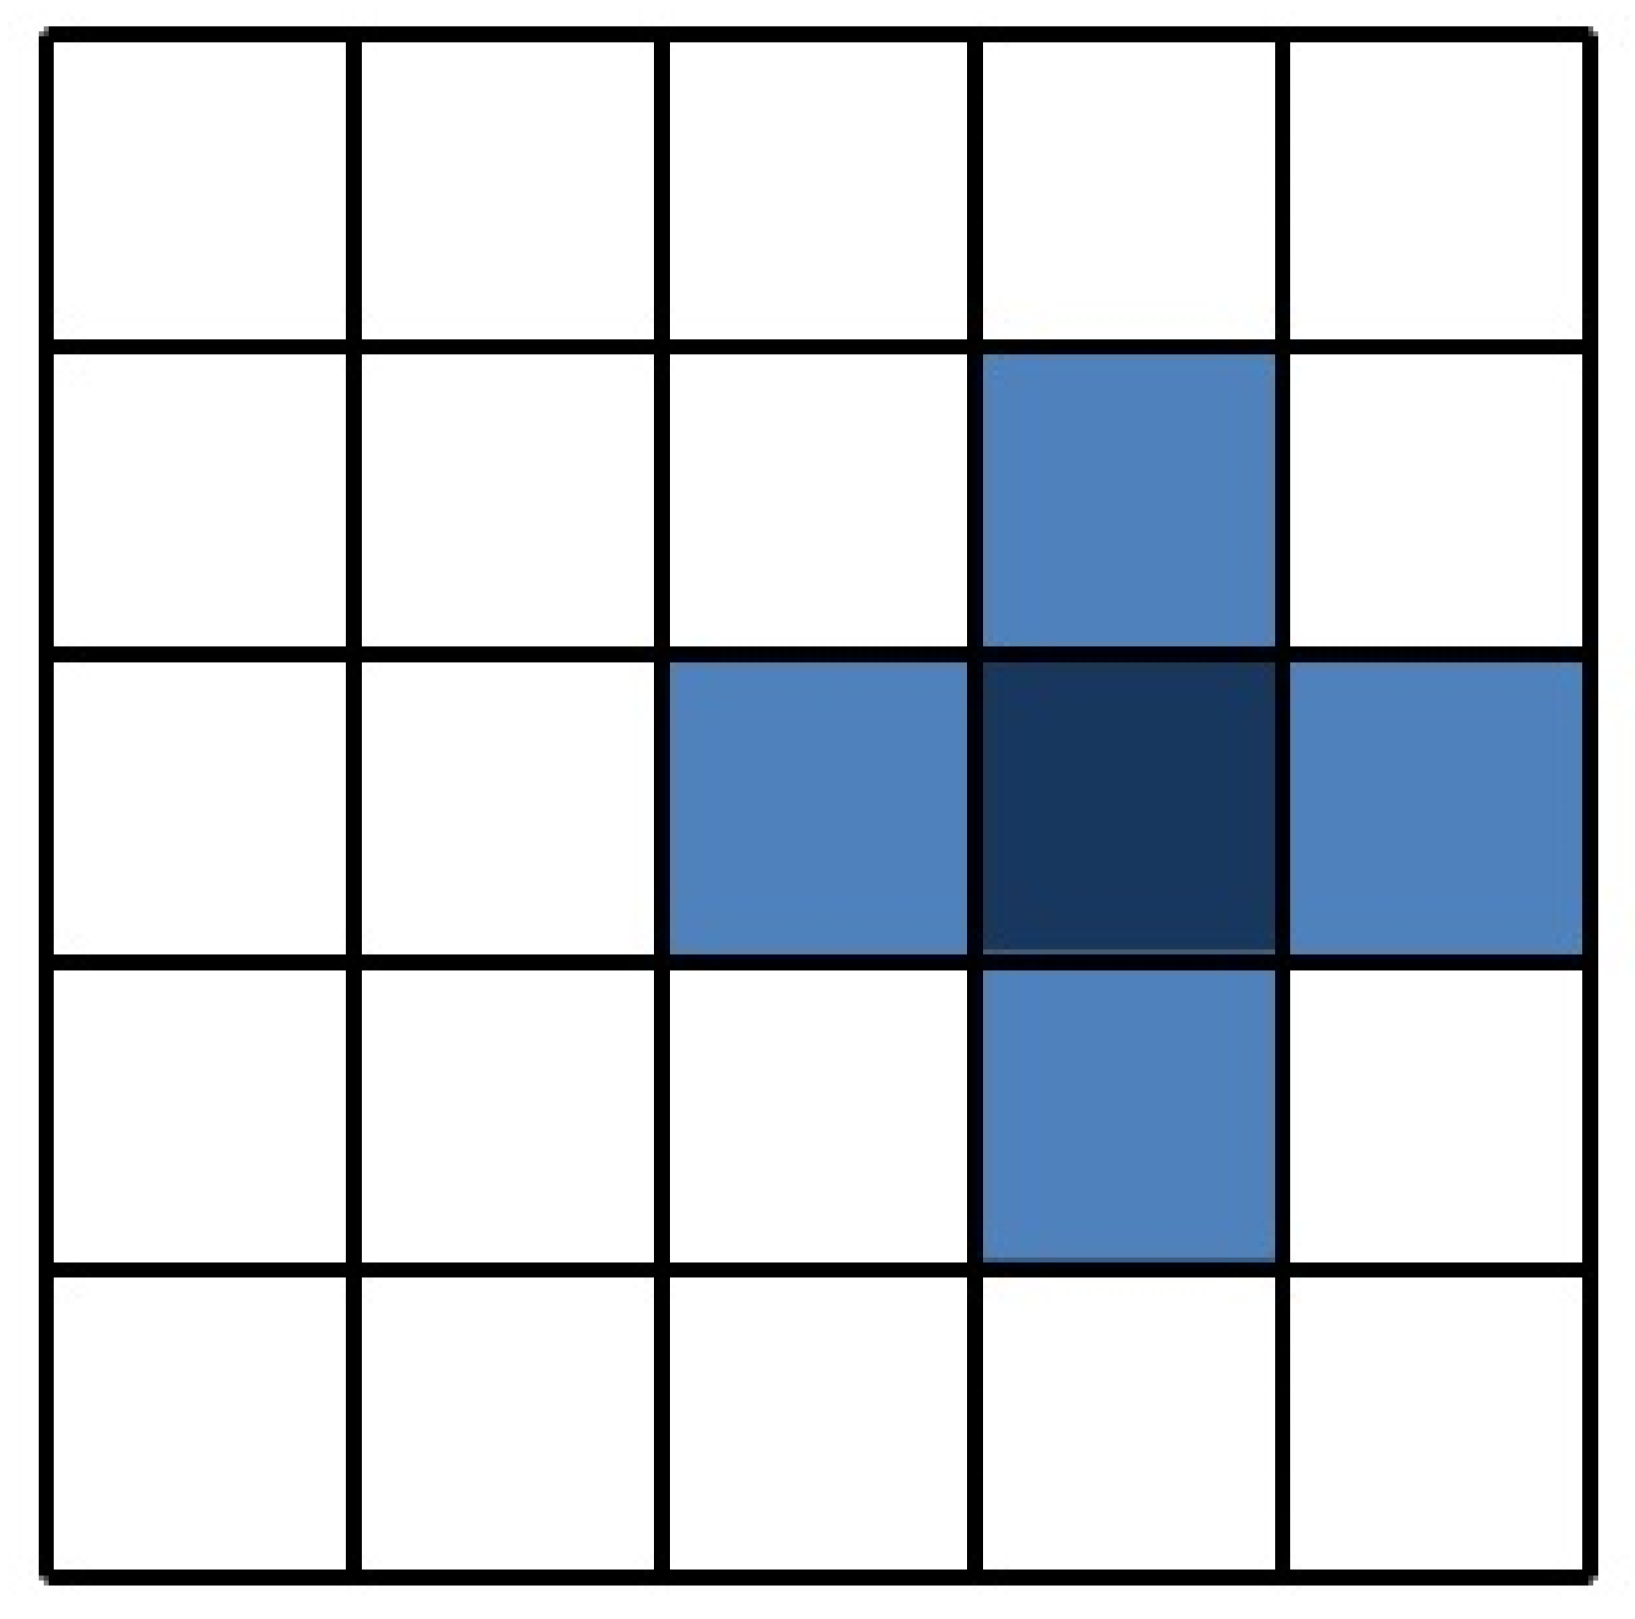
\includegraphics[width=0.5\textwidth]{imm/tep/tep1.png}  
	\caption{Transport Equation Problem for a single cell} 
	\label{tep1}
\end{figure}
After that, the cells near the boundary copy the calculated values to the boundary cells:
\begin{figure}[h!]
	\centering
	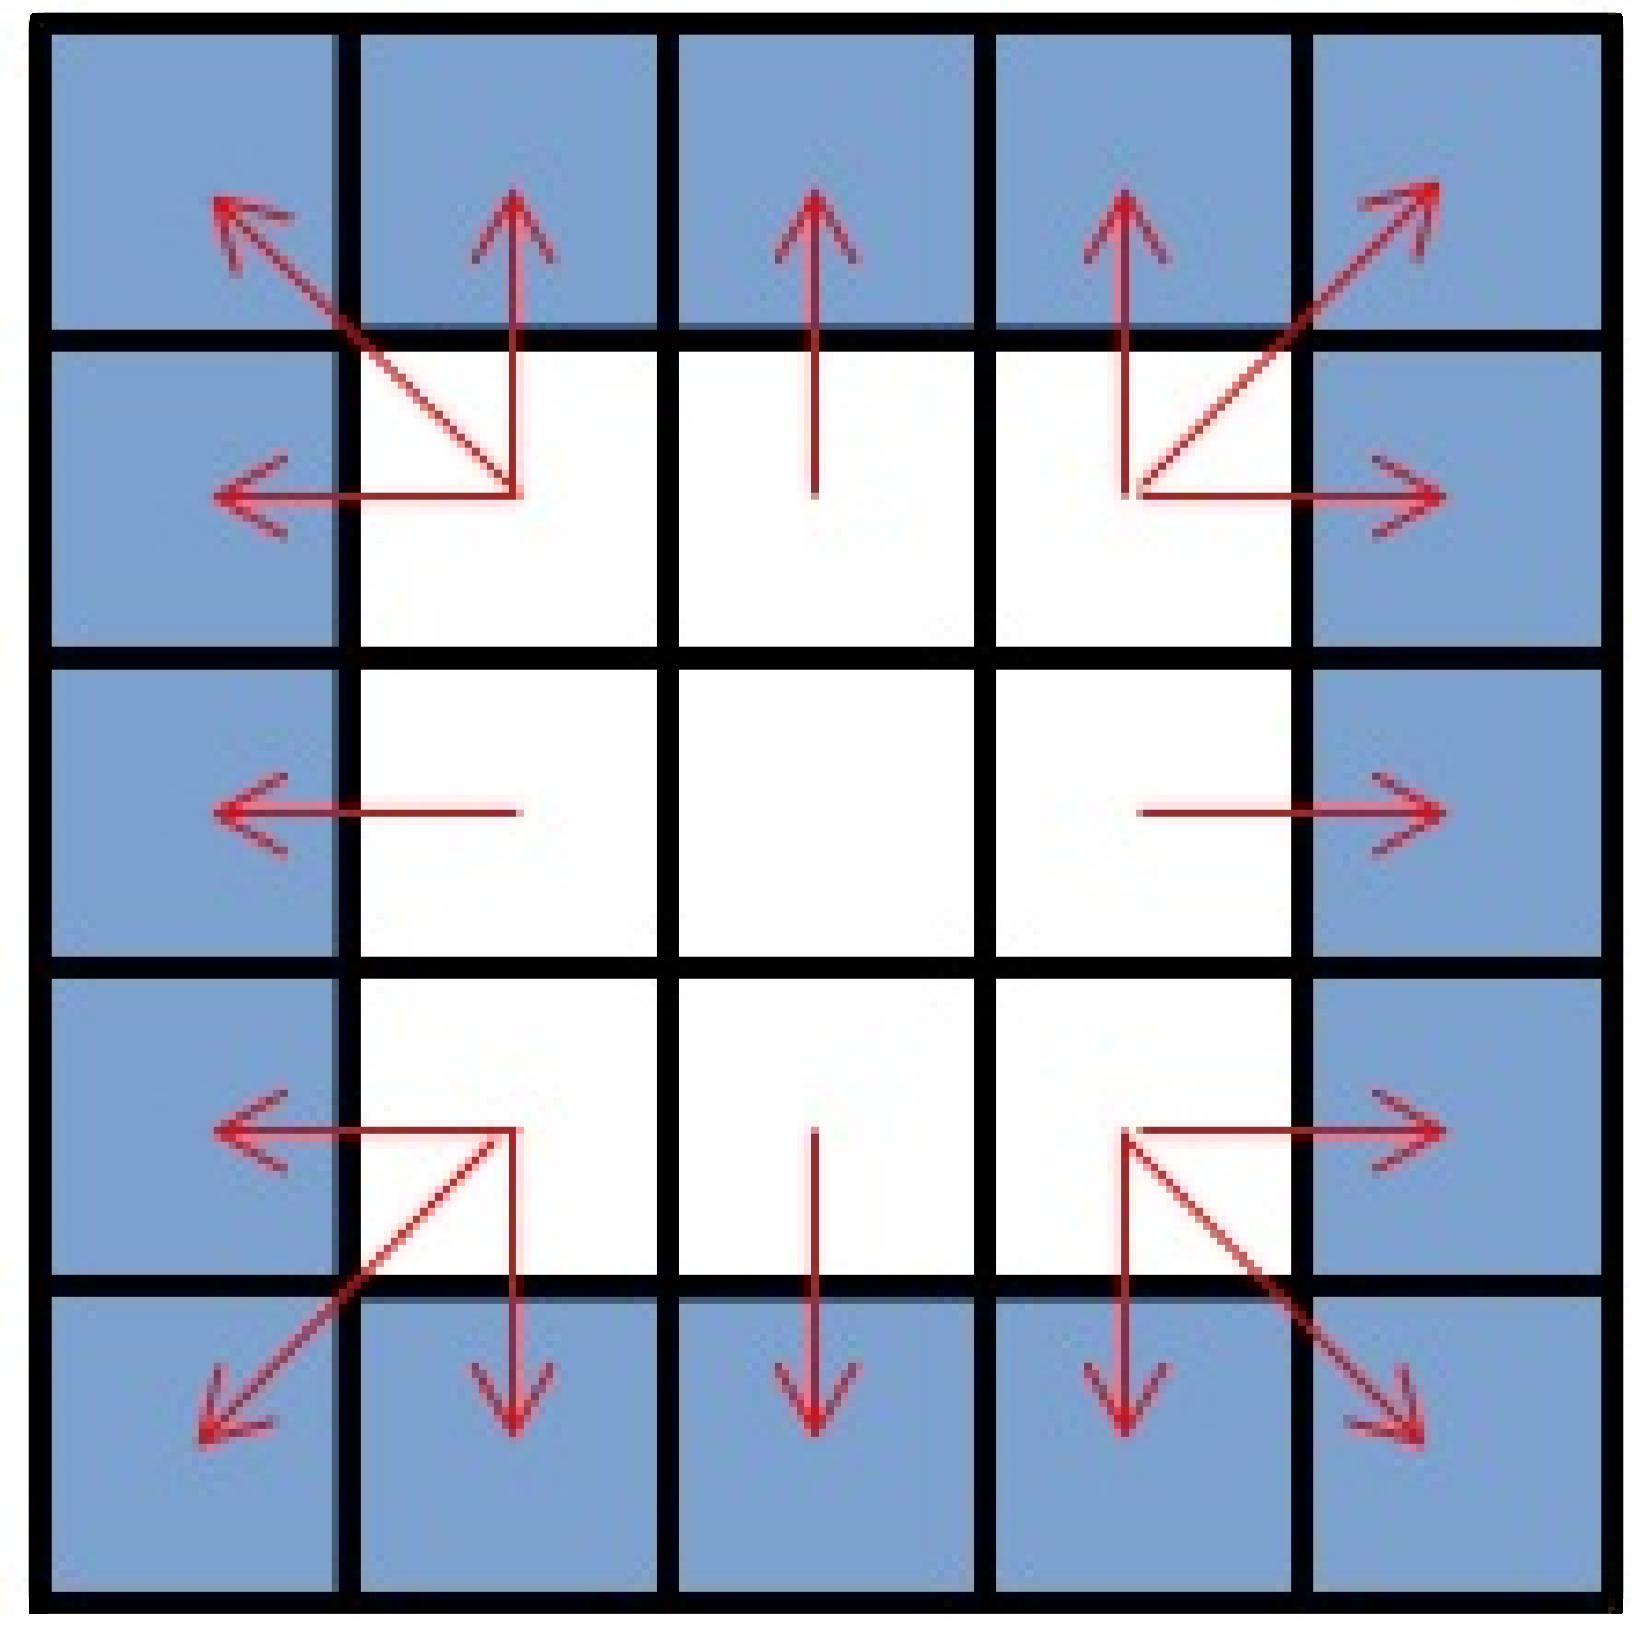
\includegraphics[width=0.5\textwidth]{imm/tep/tep2.png}  
	\caption{Propagarting the values to the boundary} 
	\label{tep2}
\end{figure}

\section{Hardware Implementation}
Since each cell has to compute the same equation, and since there is no data dependencies between them, we can implement a component that compute this result. Let's call it \textit{tep\_unit}.
The \textit{tep\_unit} has as input
\begin{itemize}
\item t0: the value of the interested cell
\item tr: the value of the cell on the right side
\item tup: the value of the cell on the upper side
\item tl: the value of the cell on the left side
\item tdn: the value of the cell on the lower side
\item alpha : the value of theconstant
\end{itemize}
with these values, it is possible to  calculate the final value.\\
The equation above can be rewritten as :
\begin{equation} \label{tep_eq2}
temp = t_{0}+\alpha{[t(i-1,j)+t(i,j-1)]-[t(i+1,j)+t(i,j + 1)]}
\end{equation}
For the cell on the border or on the angle of the matrix, we will compute the equation as if there were some zero cells in the neighborhood.
In fig. \ref{tep_unit} we can see the DFG.
\begin{figure}[h!]
	\centering
	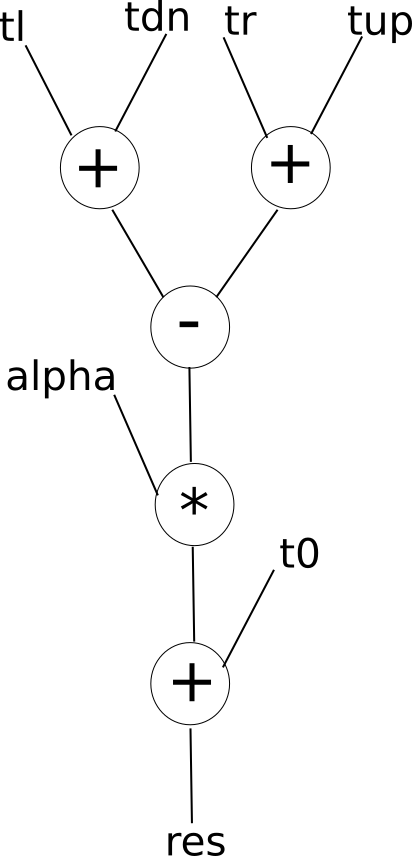
\includegraphics[width=0.4\textwidth]{imm/tep/tep_unit0.png}  
	\caption{Tep\_unit DFG} 
	\label{tep_unit}
\end{figure}

\clearpage
\newpage
\section{Simulation}
The simulation shown in this work has a 4x4 matrix  (fig. \ref{fig:tep_sim}, highlighted in yellow)
\begin{center}
	$\begin{bmatrix}
	1 & 2& 3&4\\
	3&4&2&8\\
	5&6&1&18\\
	7&8&0&22
	\end{bmatrix}$
\end{center}
\begin{figure}[h!]
	\centering
	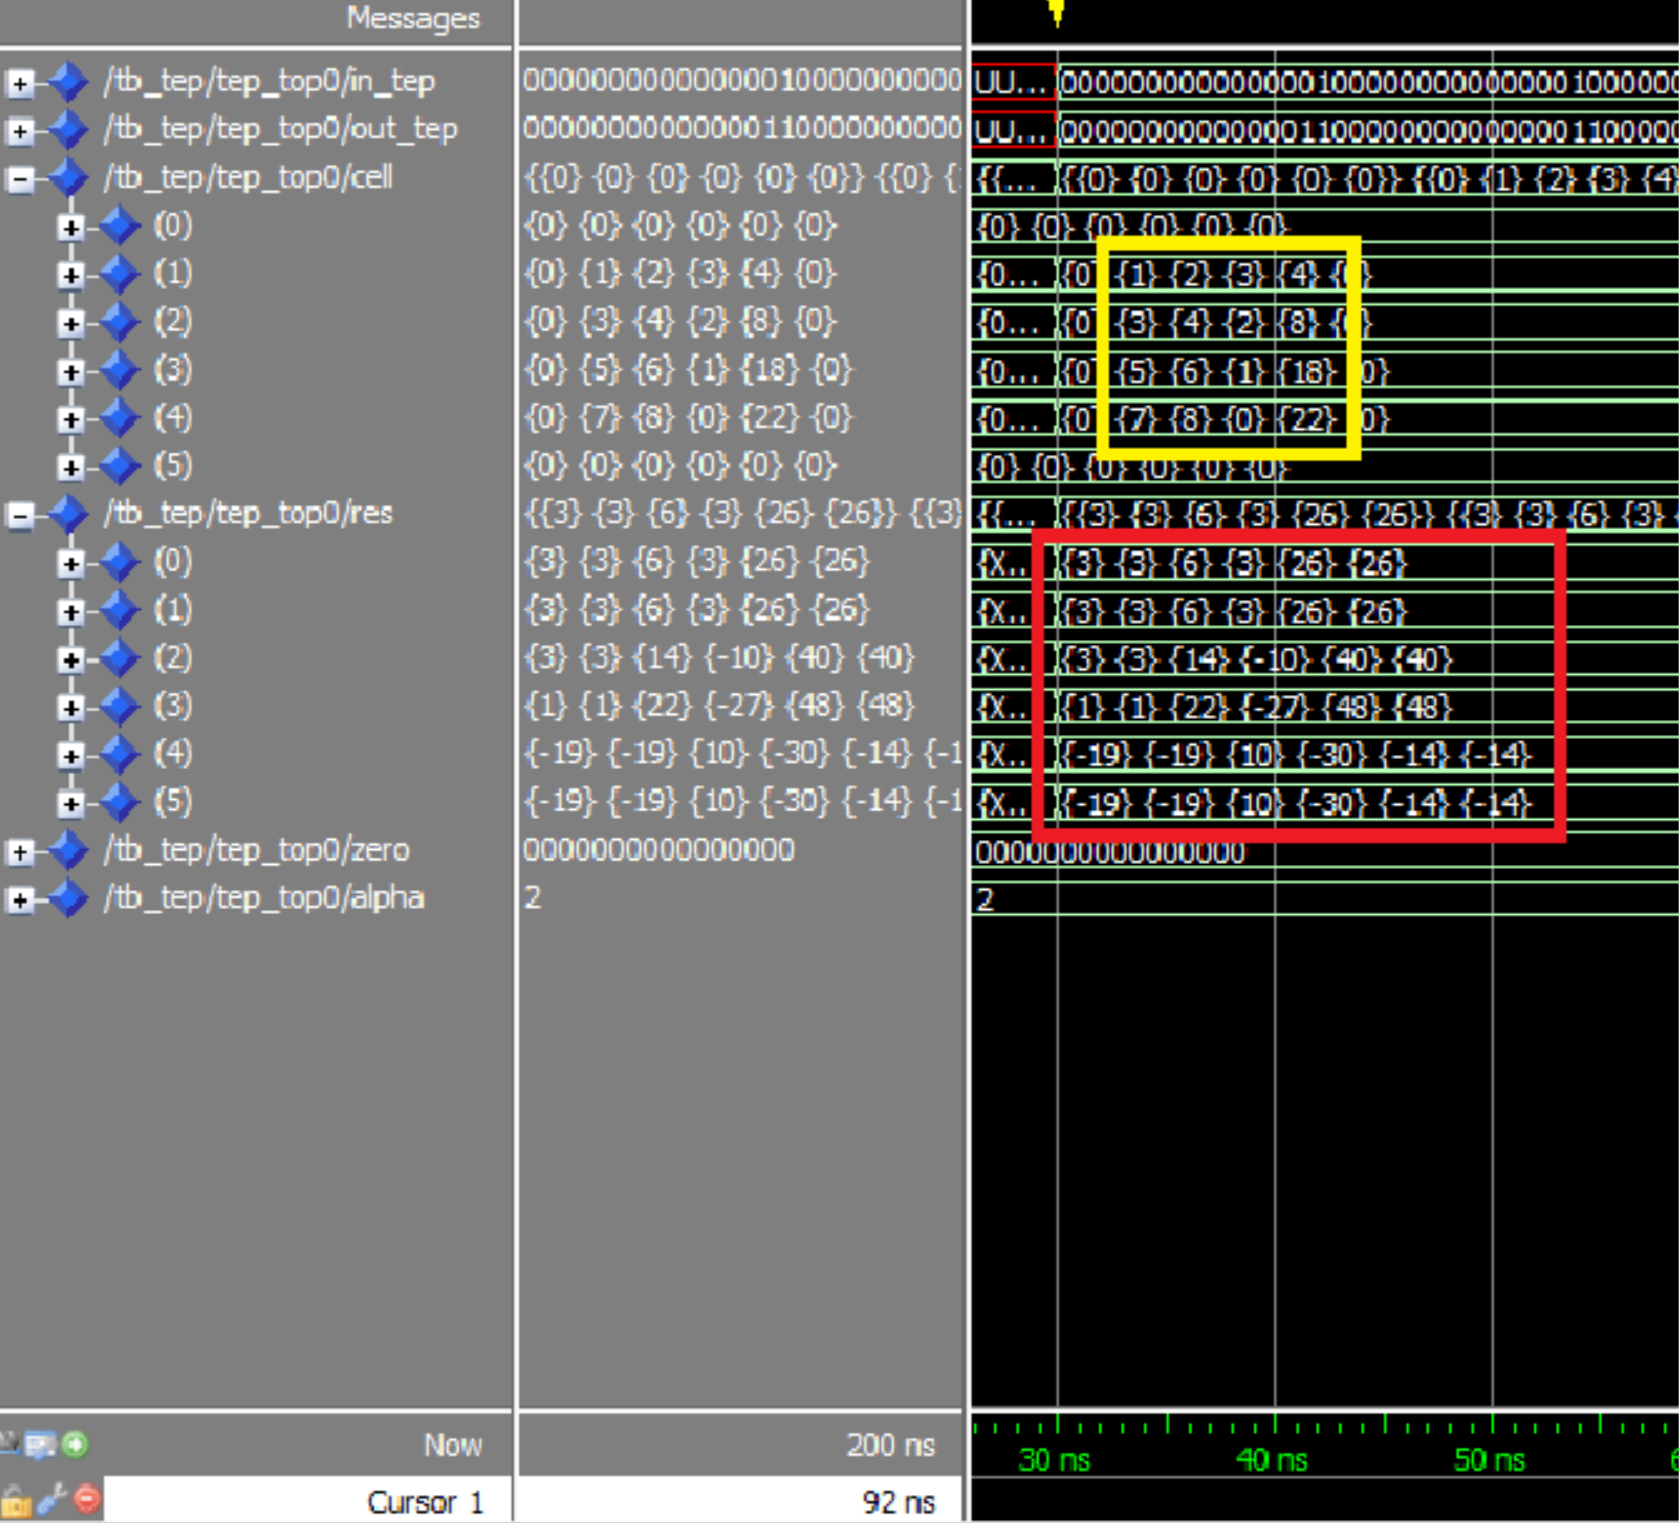
\includegraphics[width=\textwidth]{imm/tep/wave_t.png}  
	\caption{Transport Equation Problem's simulation} 
	\label{fig:tep_sim}
\end{figure}
\bigskip
If we compute the equation \ref{tep_eq2} for each element we will get 
\begin{center}
	$\begin{bmatrix}
	3 & 6& 3&26\\
	3&14&-10&40\\
	1&22&-27&48\\
	-19&10&-30&-14
	\end{bmatrix}$
\end{center}
\bigskip
Now we have to propagate the values on the border to the boundary, thus having
\begin{center}
	$\begin{bmatrix}
	3&3 & 6& 3&26&26\\
	3&3 & 6& 3&26&26\\
	3&3&14&-10&40&40\\
	1&1&22&-27&48&48\\
	19&-19&10&-30&-14&-14\\
	19&-19&10&-30&-14&-14
	\end{bmatrix}$
\end{center}
\bigskip
\section{Comparison with LIM's architecture}
I take the results of the LIM's architecture. 
The pseudocode for the LIM architecture is the following:
\begin{enumerate}
 \item Each cell reads its own value; 
 \item Reads N-W-S-E cells data (4 different values);
 \item Computes sums/subtractions and a multiplication; 
 \item Boundary cells just copy their neighbours' values;
 \item Writes the final result in its own memory;
\end{enumerate}
As already said, the main advantage of the LIM architecture is the parallelism: the presence of many cells that can work autonomously greatly increases the speed of the computation of algorithms that can be executed in parallel.\\
In particular, the duration of the algorithms doesn't depend on the number of cells composing the grid.
The total duration for the computation is equal to:
\begin{itemize}
\item $ N $ clock cycles to write the data;
 \item $ 16 \cdot i  $clock cycles to compute the algorithm;
 \item $ 2N+1 $ clock cycles to read the data through a remote read.\\
\end{itemize}
Therefore,
\begin{center}
	$ t =  N + 16\cdot i +2N +1=3N + 16\cdot i +1  $
\end{center}
   \begin{center}
   	\begin{tabular}{ | p{1.8cm} | >{\centering\arraybackslash}p{6cm} | >{\centering\arraybackslash}p{6cm} | }
   		\hline
   		\label{table:tep_tab} & LIM & This work \\
   		\hline
   		Area & $ N^{2}$  cells   & $3N^{2}
   		$  adders, $N^{2}$ substractors, multipliers \\
   		\hline
   		Time & $3N + 16\cdot i +1 $&
   		
   		(time for 3 additions) + time for a single multiplication 
   		\\
   		\hline
   		
   	\end{tabular}
   \end{center}
\chapter{Magnetostatic field calculation 3D}
To compute the total magnetostatic energy, the ferromagnetic systems can be discretized as three-dimensional cubes.\\
  
\begin{figure}[h]
	\centering
	\includegraphics[width=0.7\textwidth]{imm/3d/cube.pdf}  
	\caption{The selected cell is supposed to sum all the magnetostatic field contributions between it and all the other cells}
	\label{fig:cube}
\end{figure}
  The following is the implementation of an algorithm shown in the paper \cite{3dtesi}, related to the evaluation of the contribution of the magnetostatic field to the total energy of a system. \\In general, the magnetostatic field is connected to the magnetization $ [\overrightarrow{M}] $ through the magnetizing tensor [\textbf{TG}].
  
  
  The evaluation of the magnetostatic field of a given cell requires the summation on all cells of the mesh due to the the long range of the dipole interaction.
  
  \begin{equation} \label{3d_formula}
  \overrightarrow{H}(ijk)=-M_{s}\sum\limits_{i'=1}^{N_{x}} \sum\limits_{j'=1}^{N_{y}}\sum\limits_{k'=1}^{N_{z}}\begin{bmatrix}
  TG_{xx} & TG_{xy} & TG_{xz}\\
  TG_{yx} & TG_{yy}& TG_{yz}    	\\
  TG_{zx}&TG_{zy} & TG_{zz}  
  \end{bmatrix}_{(i-i',j-j',k-k')}\begin{bmatrix}
  m_{x}\\
  m_{y}\\
  m_{z}\end{bmatrix}_{(i',j',k')}
  \end{equation}
  
  \section{Product TG and M}
  Each cell $ (i'j'k') $ has a finite state machine that evaluates the magnetostatic field contribution between the cell \textit{ijk} and the cell \textit{i'j'k'}.
  \begin{center}
  		$ \overrightarrow{h}(i-i',j-j',k-k')= \begin{bmatrix}
  	TG_{xx} & TG_{xy} & TG_{xz}\\
  	TG_{yx} & TG_{yy}& TG_{yz}    	\\
  	TG_{zx}&TG_{zy} & TG_{zz}  
  	\end{bmatrix}_{(i-i',j-j',k-k')}\begin{bmatrix}
  	m_{x}\\
  	m_{y}\\
  	m_{z}\end{bmatrix}_{(i',j',k')}$
  \end{center}.
  
  The matrix \textbf{TG}$ _{(i-i',j-j',k-k')} $ is the magnetizing tensor between the 2 cells, while $ \overrightarrow{M}_{(i',j'k')} $ is the magnetization of the cell $ i',j',k'$.\\\\
  The FSM is composed by the following states:
  \begin{itemize}
  	 \item \textbf{READ\_MX}: save $ m_x $ value
  	 \item \textbf{READ\_MY}: save $ m_y $ value
  	 \item \textbf{READ\_MZ}: save $ m_z $ value
  	 \item \textbf{READ\_TGxx}: read $ TG_{xx} $ value and computing $ op1= TG_{xx}\cdot m_x$
  	 \item \textbf{READ\_TGxy}: read $ TG_{xy} $ value and computing $ op2= TG_{xy}\cdot m_y$
  	 \item \textbf{READ\_TGxz}: read $ TG_{xz} $ value and computing $ h_x= TG_{xz}\cdot m_z +op1+op2$.
  	 \item \textbf{READ\_TGyx}:read $ TG_{yx} $ value and computing $ op1= TG_{yx}\cdot m_x$
  	 \item \textbf{READ\_TGyy}:read $ TG_{yy} $ value and computing $ op2= TG_{yy}\cdot m_y$
  	 \item \textbf{READ\_TGyz}: read $ TG_{yz} $ value and computing $ h_y= TG_{yz}\cdot m_z +op1+op2$
  	 \item \textbf{READ\_TGzx}:read $ TG_{zx} $ value and computing $ op1= TG_{zx}\cdot m_x$
  	 \item \textbf{READ\_TGzy}:read $ TG_{zy} $ value and computing $ op2= TG_{zy}\cdot m_y$
  	 \item \textbf{READ\_TGzz}: read $ TG_{zz} $ value and computing $ h_z= TG_{zz}\cdot m_z +op1+op2$
  \end{itemize}
   
     \section{Logic Plane}
     This component groups all the cells in a given plane, and enables the computation of the magnetostatic field contributions between the cell \textit{ijk} and all the cells in a given plane (i.e. $ k $ is fixed).
     \begin{center}
     	$ \overrightarrow{h}(i-i',j-j',k-k^*)$\quad \quad $ \forall i'<N_x,$\quad $ j'<N_y,$ \qquad $ k=k^* $\\
     	   \end{center}
     	   which can be also seen as	$ \overrightarrow{h}(i-i',j-j',k-k^*)$ and can be computed as
     	      \begin{center}
     	$ \begin{bmatrix}
     	TG_{xx} & TG_{xy} & TG_{xz}\\
     	TG_{yx} & TG_{yy}& TG_{yz}    	\\
     	TG_{zx}&TG_{zy} & TG_{zz}  
     	\end{bmatrix}_{(i-i',j-j',k-k^*)}\begin{bmatrix}
     	m_{x}\\
     	m_{y}\\
     	m_{z}\end{bmatrix}_{(i',j',k^*)} $ \quad \quad $ \forall i'<N_x,$ \quad $ j'<N_y,$ 
     \end{center}
          All this computation can be done in parallel. 
          
          \begin{figure}[h]
          	\centering
          	\includegraphics[width=0.9\textwidth]{imm/3d/logic_plane1.png}  
          	\caption{Magnetostatic field of each cell in a given plane}
          	\label{fig:logic_ plane}
          \end{figure}
    \section{Sum all}
    The \textit{sum\_all} is a component that given a fixed $ k^* $ (i.e. a given plane) evaluates the magnetostatic field of all cells in a fixed plane.
    The input is given by the \textit{logic plane}, as shown in the fig. \ref{fig:logic_ plane}.
    \begin{center}
    	$ \sum\limits_{i'=1}^{N_{x}} \sum\limits_{j'=1}^{N_{y}}\begin{bmatrix}
    	TG_{xx} & TG_{xy} & TG_{xz}\\
    	TG_{yx} & TG_{yy}& TG_{yz}    	\\
    	TG_{zx}&TG_{zy} & TG_{zz}  
    	\end{bmatrix}_{(i-i',j-j',k-k^*)}\begin{bmatrix}
    	m_{x}\\
    	m_{y}\\
    	m_{z}\end{bmatrix}_{(i',j',k^*)} $
    \end{center}
    By looking to the formula \ref{3d_formula}, we have to evaluate the sum for each plane, so we store this sum and wait for the next plane to be computed and added to the previous sum.\\
    Of course when we reach the $ k^{th} $ plane, we stop the sum and we set a signal to tell that the calculation is finished.\\
    Overall, this component perform the following computation\\
    \begin{center}
    	$ \sum\limits_{k'=1}^{N_{z}}\begin{pmatrix}
    	\sum\limits_{i'=1}^{N_{x}} \sum\limits_{j'=1}^{N_{y}}\begin{bmatrix}
    	TG_{xx} & TG_{xy} & TG_{xz}\\
    	TG_{yx} & TG_{yy}& TG_{yz}    	\\
    	TG_{zx}&TG_{zy} & TG_{zz}  
    	\end{bmatrix}_{(i-i',j-j',k-k')}\begin{bmatrix}
    	m_{x}\\
    	m_{y}\\
    	m_{z}\end{bmatrix}_{(i',j',k')}
    	\end{pmatrix} $
    \end{center}
    \bigskip
\section{Simulation and Test}
I wrote a testbench to check the correct behaviour of this architecture.
\subsection{Testbench of the cell} \label{tb_cell_3d}
First we check that the component \textit{cell} is working according to the specifications.
We can distinguish the 4 main phase of this test as shown in fig. \ref{fig:tb_cell_phases}.
  \begin{figure}[h]
  	\centering
  	\includegraphics[width=\textwidth]{imm/3d/tb_cell_phases.png}  
  	\caption{The phases of a single cell}
  	\label{fig:tb_cell_phases}
  \end{figure}
The 4 phases are
\begin{enumerate}
	\item \textbf{Reading the magnetization}: here we read the magnetization in the 3 direction. 
	This phase is highlighted in yellow in the figure.\\ \ref{fig:tb_cell_phases}.
	$ m_x=1 $, $ m_y=2 $, $ m_z=3 $, 
	\item \textbf{Reading the magnetization x-axis}: Reading the magnetizing tensor contributions between 2 cells. Right now we look only to the contributions along the x-axis with the x-axis, y-axis, z-axis.\\In the meantime we can evaluate the magnetostatic field $ h_{x} $.
	This phase is highlighted in blue in the figure.\\
	$ tg_{xx}=4 $, $ tg_{xy}=5 $, $ tg_{xz}=6 $\\
	$ op1=m_x \cdot tg_{xx}=4 $\\
	$ op2=m_y \cdot tg_{xy}=10 $\\
	$ h_x=op1+op2+m_z \cdot tg_{xz}=32$\\
	$ output=h_x=32$
	\item \textbf{Reading the magnetization y-axis}: Similarly as the previous phase, we look only to the magnetizing tensor contributions along the y-axis with the x-axis, y-axis, z-axis.\\In the meantime we can evaluate the magnetostatic field $ h_{y} $.
	This phase is highlighted in red in the figure.\\
	$ tg_{yx}=7 $, $ tg_{yy}=8 $, $ tg_{yz}=9 $\\
	$ op1=m_x \cdot tg_{yx}=7 $\\
	$ op2=m_y \cdot tg_{yy}=16 $\\
	$ h_x=op1+op2+m_z \cdot tg_{yz}=50$\\
	$ output=h_x=50$
	\item \textbf{Reading the magnetization z-axis}: Similarly as the previous phase.
	This phase is highlighted in pink in the figure.\\
	$ tg_{yx}=10 $, $ tg_{yy}=11 $, $ tg_{yz}=12 $\\
	$ op1=m_x \cdot tg_{yx}=10 $\\
	$ op2=m_y \cdot tg_{yy}=22 $\\
	$ h_x=op1+op2+m_z \cdot tg_{yz}=68$\\
	$ output=h_x=68$
\end{enumerate}
After these 4 phases, the cell starts again from phase 1 as shown in fig. \ref{fig:tb_cell}.
\begin{figure}[h]
	\centering
	\includegraphics[width=\textwidth]{imm/3d/tb_cell.png}  
	\caption{Testbench of a single cell}
	\label{fig:tb_cell}
\end{figure}
\subsection{Testbench of the Top entity}
After testing the \textit{cell} components, we integrate them (\textit{logic\_plane}) with the \textit{sum\_all} accumulator.\\
The \textit{logic\_plane} and the \textit{sum\_all} components have to be synchronized, so a delay is needed (i.e. the logic plane evaluate the magnetostatic field of a plane and then the accumulator is ready to sum).\\
For simplicity, we test the behaviour of a parallelepiped which base is 2x2 and which height is 4.

\begin{figure}[h]
	\centering
	\includegraphics[width=\textwidth]{imm/3d/tb_3d_top.png}  
	\caption{Testbench of the top entity - first plane}
	\label{tb_3d_top}
\end{figure}
As we can see in the fig. \ref{tb_3d_top}, in the first 3 clock cycles we see the input   $m_x$, $ my$, $mz $ (\textit{tb\_tg\_top\_2d/dut/tg\_logic/input} signal) of each of the 4 cells of the first plane.\\
In the next 9 clock cycles we have all the 9 values of the  \textbf{TG}  matrix (\textit{tb\_tg\_top\_2d/dut/tg\_logic/input} signal). When we have the required input we can compute the output value $ h_x $, $ h_y $, $ h_z $ of each cell (in the signal \textit{tb\_tg\_top\_2d/dut/tg\_logic/output} we have  $ h_x $ at 23 ns, $ h_y $ at 29 ns, $ h_z $ at 35). To better understand the FSM see the testbench of a single cell (\ref{tb_cell_3d}), the only difference is that now we have 4 cells (2x2 matrix) computing in parallel.\\
When we have all the cells $ h_x $, $ h_y $, $ h_z $ values, we can compute the  $ H_x $, $ H_y $, $ H_z $ of the plane. In the figure \ref{tb_3d_top}, at 25 ns we have the $H_x$ value of the first plane which is given by the sum of the $h_x$ values computed by the cells (32+24+54+0=110). Same thing for $H_y$ and $H_z$.\\
Without doing any more tedious calculations, we can see in fig. \ref{tb_3d_acc} that we accumulate the $ H_x $, $H_y$, $H_z$ values of each plane in order to get the final value\textbf{  $ \overrightarrow{H} $ } of the whole parallelepiped.
\begin{figure}[h]
	\centering
	\includegraphics[width=\textwidth]{imm/3d/tb_3d_acc.png}  
	\caption{Testbench of the top entity - whole parallelepiped}
	\label{tb_3d_acc}
\end{figure}
\clearpage
\newpage 
\section{Characteristics of Magnetostatic field calculation 3D}
\vspace{10pt}
{\large \textbf{PROCESSING ELEMENTS}}\vspace{10pt}\\
\begin{tabular}{ p{0.2cm} p{14.5cm}}
	
	&\textbf{1- Which kind of Processing element?}\\
	&	Adder, multiplier\vspace{7pt}\\
	&	\textbf{2- Functionality}\\
	&	Addition, multiplications (Evaluatin the multiplication between matrix and vectors. Another function is the accumulator.).\vspace{7pt}\\
	&	\textbf{3- Complexity}\\
	&	\begin{tabular}{ p{0.2cm} p{1.2cm}  p{13cm}}
		
		& Area: &$ i\cdot j $ cells\\
		& & one accumulator\\
		& Time: & (12 clock cycles)$\cdot k$\vspace{3pt}\\
		
		
	\end{tabular}\vspace{7pt}\\
	&	\textbf{4- Parallelism}\\
	&	Each cell can evaluate their magnetostatic contributions.\vspace{7pt}\\
	&	\textbf{5-Reconfigurability}\\
	&	No\vspace{7pt}\\
	&	\textbf{6- Programmability}\\
	&	No\vspace{7pt}\\
	&	\textbf{7- Need a dedicated memory?}\\
	&	Yes, to store the magnetization values ($m_x, m_y, m_z$)\vspace{7pt}\\
	&\textbf{8- Relationship with I/O}\\
	&	INPUT: values of the magnetization values, magnetizing tensor of each cells.\\
	&	OUTPUT: result of the magnetostatic field. algorithm\end{tabular}\vspace{74pt}\\
\newpage{\large \textbf{\qquad }}\vspace{10pt}\\
{\large \textbf{MEMORY ELEMENTS}}\vspace{10pt}\\\begin{tabular}{ p{0.2cm} p{14.5cm}}
	&\textbf{1- Need a clever memory LIM?}\\
	&	No, but can be implemented\vspace{7pt}\\
	&\textbf{2- Is there a data search algorithm?}\\
	&	No\vspace{7pt}\\
	&\textbf{	3-Interface mechanism with other PE or memories}\\
	&	No\vspace{7pt}\\
	&	\textbf{4- Access mechanism}\\
	&	(No memory for this implementation)\vspace{7pt}\\
	&	\textbf{5- Hierarchization} \\
	&	(No memory for this implementation)\vspace{7pt}\\
	&\textbf{	6- Cache coherency} \\
	&	(No memory for this implementation)\vspace{7pt}\\
	&\textbf{	7- Is it a a transactional memory?}\\
	&	(No memory for this implementation)\vspace{7pt}\\
	&\textbf{	8- Are there virtualization (paging) mechanisms?}\\
	&	(No memory for this implementation)\end{tabular}\vspace{14pt}\\
\vspace{10pt}\\
{\large\textbf{ENCODING INFORMATION}}\vspace{10pt}\\
\begin{tabular}{ p{0.2cm} p{14.5cm}}
	&\textbf{1-Which encoding is used?}\\
	&Binary encoding
\end{tabular}
\newpage{\large\textbf{ }}\vspace{10pt}\\
{\large\textbf{CONNECTIONS}}\vspace{10pt}\\\begin{tabular}{ p{0.2cm} p{14.5cm}}
	&\textbf{1-Packet Exchange Protocol}\\
	&Directly\vspace{7pt}\\
	&\textbf{2-Timing (asynchronou/synchronous)}\\
	&Synchronous\vspace{7pt}\\
	&\textbf{3-Are there multiple instances? }\\
	&Yes\vspace{7pt}\\
	&\textbf{4-Heterogeneity (Local/Distant I/O Connections)}\\
	&Heterogeneous when storing the values from the Input connections.\vspace{7pt}\\
	&\textbf{5-Are there any buffers?}\\
	&No.
\end{tabular}\vspace{14pt}\\

%\chapter{}
\section{Substitutional matrix}
How to quantify the amino acids similarity? This is the question that the biologists set themselves when they started thinking about substitutional matrix.
The substitutional matrices are based on the probability that an AA is substituted with another during evolution. These matrices assign to each pair of AAs, a value that indicates the degree of similarity. They are obtained with statistical methods that reflect the frequency with which each AA is replaced by another in homologous proteins families [13]. A positive value in the matrix (Fig. 2.6) means that the two amino acids are similar and they are frequently exchanged each other. \\
The most common used substitutional matrices are PAM and Blosum.
\subsection{BLOSUM matrix}
The BLOSUM matrices were introduced in 1992 by Henikoff & Henikoff [15] to give a score for substitution in the amino acid sequence comparisons.
BLOSUM (BLOck SUbstitution Matrix) matrices are constructed using multiple alignments of evolutionarily divergent proteins. The probabilities used in the matrix calculation are computed by looking at ”blocks” of conserved sequences found in multiple protein alignments. Each block normally refers to a set of proteins in relation to each other. When the frequency of replacement within a family is determined, is possible to individuate the significant substitutions. By means of aggregation techniques, all sequences contained in a block are put together into the groups. The numerical value associated to the matrices (eg BLOSUM62) represents the threshold value applied by the method of aggregation. A value of 62 indicates that the sequences are put together in the same group if they have an identity value equal to or greater than 62%. Lower values of threshold (eg BLOSUM45) indicate that they have been grouped sequences that are more distant evolutionarily.

\section{Smith-Waterman local alignment method}
2.3.2.1 Smith-Waterman
Smith and Waterman in 1981 described a Local alignment method [24] which was a variation of N-W algorithm. Aim of this method is to find common regions between two protein (Qry, Sbj) through calculation of similarity score. The local methods usage are indicated when long biological sequences are compared. Since in these cases, Global alignment can lead to weak correlation when comparing two highly diverged sequences where only part of them are aligned [25]. S-W, as N-W, is a dynamic programming algorithm (Fig. 2.13) that works with a score matrix (N+1 * M+1) where first row and column are initialized to zeros. This algorithm can be substantially described in three steps:

%\chapter{Singular Value Decomposition}

Given a complex matrix $ A $ having \textit{m} rows and $ n $ columns, the matrix product $ U\Sigma V^T $ is a singular value
decomposition for a given matrix $ A $ if
\begin{itemize}
\item $ U $ and $ V $, respectively, have orthonormal columns. 
\item $\Sigma$  has nonnegative elements on its principal diagonal and zeros elsewhere.
\item $ A=U\Sigma V^T $
\end{itemize}
One application of the SVD is data compression. Consider some matrix $ A $ with rank five hundred; that is, the columns of this matrix span a 500-dimensional space. Encoding this matrix on a computer is going to take quite a lot of memory! We might be interested in approximating this matrix with one of lower rank. How close can we get to this matrix if we only approximate it as a matrix with rank one hundred, so that we only have to store a hundred columns?\\
It turns out that you can prove that taking the $ n $ largest singular values $ A $, replacing the rest with zero (to form $ \Sigma $), and recomputing $U\Sigma V^T $ gives you the provably best $ n $-rank approximation to the matrix.


It means that we can take a list of RR unique vectors, and approximate them as a linear combination of KK unique vectors.

https://www.quora.com/What-is-an-intuitive-explanation-of-singular-value-decomposition-SVD
\section{Example of a SVD computation}

For simplicity, we compute the SVD of a 2x2 matrix C:
\begin{center}
	$ 
	C=\begin{bmatrix}
	5 &   5 \\
-1  &  7 \\
	\end{bmatrix}$
\end{center}
and we want to write it as $ C=U\Sigma V^{T} $.\\
We have to take into account these 2 equations:
\begin{itemize}
	\item $ C^T C = V\Sigma^T\Sigma V^T$
	\item $CV=U\Sigma$
\end{itemize}
We first use the first equation  $ C^T C = V\Sigma^T\Sigma V^T$, and find the eigenvalues and the eigenvectors of $C^T C $.
The eigenvalues will be the entries of the diagonal entries of $ \Sigma^T\Sigma $, while the eigenvectors will be the entries of $ V $.\\
Let's compute $ C^T \cdot C $\\
\begin{center}
	$ C^T \cdot C =\begin{bmatrix}
5 &   -1 \\
5  &  7 \\
\end{bmatrix}\begin{bmatrix}
5 &   5 \\
-1  &  7 \\
\end{bmatrix}=\begin{bmatrix}
26 &   18 \\
18  &  74 \\
\end{bmatrix}$\\
\end{center}
Now we can find the eigenvalues of the matrix $ C^T \cdot C $.\\
We know that an eigenvalue of $ C^T \cdot C $, is a solution of the polynomial equation $det( C^T \cdot C-\lambda I)=0 $, where $ I $ is the identity matrix.\\
\begin{center}
	$det( C^T \cdot C-\lambda I)=det\begin{pmatrix}\begin{bmatrix}
26 &   18 \\
18  &  74 \\
\end{bmatrix}-\lambda\begin{bmatrix}
1 &   0 \\
0  &  1 \\
\end{bmatrix}\end{pmatrix}=$
\end{center}\begin{center}

=$det\begin{bmatrix}
26-\lambda &   18 \\
18  &  74-\lambda \\
\end{bmatrix}=(26-\lambda)(74-\lambda)-18\cdot 18=$
\end{center}

\begin{center}
	$= \lambda^2-100\lambda+1600 $
\end{center}
Since $ \lambda^2-100\lambda+1600 $ is a second degree equation, we can solve it using the general formula \begin{center}
	$ a\lambda^2+b\lambda+c $\end{center}

\begin{center}
		$\lambda=\dfrac{-b\pm\sqrt{b^2-4ac}}{2a}$

\end{center}
\begin{center}
	$\lambda=\dfrac{-100\pm\sqrt{100^2-4\cdot1600}}{2}$
	
\end{center}
which will provide the two solutions $ \lambda_1=20 $ and $\lambda_2=80$.\\
Now we want to find the eigenvector associated to the eigenvalue $ \lambda_1=20 $. We know that this eigenvector $ \textbf{v} $ solve the equation $ (C^T \cdot C-\lambda I)\textbf{v}=0 $ \\
\begin{center}
	$  (C^T \cdot C-\lambda_1 I)v_1= (C^T \cdot C-20 I) v_1= \begin{bmatrix}
	6 &   18 \\
	18  &  54\\
	\end{bmatrix}\begin{bmatrix}v_{1,1}\\v_{1,2}\end{bmatrix}=0 $
\end{center}
We can see it as an equations system
\begin{center}
	
$ \begin{cases} 6\cdot v_{1,1}+18 \cdot v_{1,2}=0 \\
   18\cdot v_{1,1}+54 \cdot v_{1,2}=0 \end{cases} $
\end{center}
and have $ v_{1,1}=-3 $,\quad $ v_{1,2}=1 $,\quad therefore $v_1=\begin{bmatrix}
-3\\
1
\end{bmatrix}$.\\
If we want the matrix $ V $ to be othonormal, then each vector of the matrix $ V $ has to be a unit vector (i.e. have lenght 1). To make it possible, we divide each entries of the vector by the lenght of the vector.
The lenght of $v_1$ is:
\begin{center}
	$ |v_1| = \sqrt{v_{1,1}^2+v_{1,2}^2}=\sqrt{(-3)^2+1^2}=\sqrt{10}$
\end{center}
\begin{center}
	$ v_1=\begin{bmatrix}
	\frac{-3}{\sqrt{10}}\\
	\frac{1}{\sqrt{10}}
	\end{bmatrix} $
\end{center}

Now we can do the same steps for the second eingenvector
\begin{center}
		$  (C^T \cdot C-\lambda_2 I)v_2=( C^T \cdot C-80 I) v_2= \begin{bmatrix}
		-54 &   18 \\
		18  &  -6\\
	\end{bmatrix}\begin{bmatrix}v_{2,1}\\v_{2,2}\end{bmatrix}=0  $
\end{center}
\begin{center}
	
	$ \begin{cases} -54\cdot v_{2,1}+18 \cdot v_{2,2}=0 \\
	18\cdot v_{2,1} -6 \cdot v_{2,2}=0 \end{cases} $
\end{center}
\begin{center}
	$  v_2=\begin{bmatrix}
	1\\
	3
	\end{bmatrix}$ $ \Longrightarrow $ orthonormal$ \Longrightarrow $ $v_2=\begin{bmatrix}
	\frac{1}{\sqrt{10}}\\
	\frac{3}{\sqrt{10}}
	\end{bmatrix}  $
\end{center}
Now we can write the matrix $ V $
\begin{center}
	$ V=\begin{bmatrix}
	v_1 & v_2
	\end{bmatrix}=\begin{bmatrix}
	\frac{-3}{\sqrt{10}} & \frac{1}{\sqrt{10}}\\
	\frac{1}{\sqrt{10}} &	\frac{3}{\sqrt{10}}
	\end{bmatrix} $
\end{center}
and the matrix $ \Sigma $. We know that  $ \Sigma $ is a diagonal matrix, so its transpose matrix is $ \Sigma^T= \Sigma  $, and doing $\Sigma^T \Sigma$ is the same thing of doing the square of each diagonal entries of $\Sigma$.
As said before at the beginning, the eigenvalues are the entries of $\Sigma^T \Sigma$, so to find the matrix $\Sigma$ we just need to make the square root of the eigenvalues and put them in diagonal.
\begin{center}
	$ \Sigma=\begin{bmatrix}
	\sqrt{\lambda_1} & 0\\
	0 & \sqrt{\lambda_2}
	\end{bmatrix}=\begin{bmatrix}
		\sqrt{20} & 0\\
		0 & \sqrt{80}
	\end{bmatrix}=\begin{bmatrix}
	2\sqrt{5} & 0\\
	0 & 4\sqrt{5}
	\end{bmatrix} $
\end{center}
Now we need to find the last part of the SVD, which is the matrix $ U $. To find it we use the second property listed at the beginning of this section\\
\begin{itemize}
	\item $CV=U\Sigma$
\end{itemize}
\begin{center}
	$ CV=\begin{bmatrix}
		5 &   5 \\
		-1  &  7 \\
	\end{bmatrix}\begin{bmatrix}
	\frac{-3}{\sqrt{10}} & \frac{1}{\sqrt{10}}\\
	\frac{1}{\sqrt{10}} &	\frac{3}{\sqrt{10}}
	\end{bmatrix}=\begin{bmatrix}
	-\sqrt{10} & 2\sqrt{10}\\
	\sqrt{10} &	2\sqrt{10}
	\end{bmatrix}=U\Sigma $
\end{center}
To find $U$, we have to decompose $\begin{bmatrix}
-\sqrt{10} & 2\sqrt{10}\\
\sqrt{10} &	2\sqrt{10}
\end{bmatrix}$ as the product of $U$ and $\Sigma$

\begin{center}
	 $\begin{bmatrix}
	 -\sqrt{10} & 2\sqrt{10}\\
	 \sqrt{10} &	2\sqrt{10}
	 \end{bmatrix}= \begin{bmatrix}
	 	u_{1,1} & u_{1,2} \\
	 	u_{2,1} & u_{2,2}
	 \end{bmatrix}\begin{bmatrix}
	 2\sqrt{5} & 0\\
	 0 & 4\sqrt{5}
	 \end{bmatrix}$\\
\end{center}
If we split the matrix, we obtain
\begin{center}
	
	$ -\sqrt{10}=	u_{1,1} \cdot 2\sqrt{5} + u_{1,2} \cdot 0$\quad $ \Longrightarrow $ \quad $ 	u_{1,1}=-\frac{1}{\sqrt{2}} $\\
	
	$2\sqrt{10}=	u_{1,1} \cdot 0 + u_{1,2} \cdot 4\sqrt{5}$\quad $ \Longrightarrow $ \quad $ 	u_{1,2}=\frac{1}{\sqrt{2}} $\\
	
	$ \sqrt{10}=	u_{2,1} \cdot 2\sqrt{5} + u_{2,2} \cdot 0$\quad $ \Longrightarrow $ \quad $ 	u_{2,1}=\frac{1}{\sqrt{2}} $\\
	
	$2\sqrt{10}=	u_{2,1} \cdot 0 + u_{2,2} \cdot 4\sqrt{5}$\quad $ \Longrightarrow $ \quad $ 	u_{2,2}=\frac{1}{\sqrt{2}} $\\
\end{center}

Then finally 

\begin{center}
	$ U=\begin{bmatrix}
	\frac{-1}{\sqrt{2}} & \frac{1}{\sqrt{2}}\\
	\frac{1}{\sqrt{2}} & \frac{1}{\sqrt{2}}
	\end{bmatrix} $
\end{center}
\section{Difficulties for the SVD in ASIC}
As you can see in the example above, the SVD is a complex algorithm. I had some problems in designing it in ASIC especially for a generic matrix $ n$x$n $.
In order we have
\begin{itemize}
	\item \textbf{Determinant}, find the determinant requires times and memory. Greater the dimension of the matrix, harder the computation of the determinant.
	\item \textbf{Eigenvalues} assuming we have find the Characteristic polynomial of the matrix, we will have a polynomial equation of degree $ n $, and we have to find $ n $ solutions of this polynomial in hardware.
	\item \textbf{Eigenvectors} assuming we have all the $ n $ eigenvalues, for each of the we have to solve a system of $n$ equations with $n$ variables. In total there will be $n^2$ equations to be solved.
\end{itemize}

%\chapter{Synthesis Results}
After having properly tested the architecture of each hardware implementation, the following step is its synthesis to determine the maximum clock frequency, area and power consumption.\\
The chosen sizes are smaller because I used the \textit{Pentium 4 adder} and the \textit{booth multiplier} as adder and as multiplier. Due to their complexity, the synthesys requires much time.

\section{Integral Image}
\begin{itemize}
	\item  16 
	\item size = 8x8
\end{itemize}
\begin{center}
	\begin{tabular}{  p{4.2cm} | p{6.7cm} }
			
		\hline
	 & \quad \textbf{Integral Image}\\
	 & \quad Pipelined\\
		\hline
		Total cell area & \quad37055.540208 $ \mu m^2{} $\\

		Data arrival time & \quad 0.62 $ ns  $\\
		Internal Power & \quad	3.9107$ mW $\\
		Switching Power & \quad1.8435$ mW $\\
		Total Dynamic Power & \quad5.7542$ mW $\\
		Leakage Power & \quad0.3724 $ mW $ \\
		Total Power & \quad6.1266 $ mW $\\
		\hline
		
	\end{tabular}
\end{center}
\bigskip

\section{Discrete Cosine Transformation} \label{synDCT}
For this DCT's hadware implementation (\ref{DCTH}), I synthesized both the pipeline and not pipeline architecture. I also synthesized a small version of the LLM architecture (\ref{llmarch}).
The not pipelined version, consumes more power and take a little time more than the pipelined one. However it has a smaller area due to the absence of pipeline registers.
\subsection{DCT pipelined}
\begin{itemize}
\item  8 bits for integer part
\item 8 bits for fractional part
\item size = 4
\end{itemize}
\begin{center}
	\begin{tabular}{ p{4.2cm} | p{8cm} }
		
		\hline 
		 & \quad \textbf{Discrete Cosine Transformation}\\
		& \quad Pipelined\\
		
		\hline
		Total cell area & \quad 70428.471340$ \mu m^2{} $\\

		Data arrival time & \quad 1.83 $ ns $\\
		Internal Power & \quad 4.5759$ mW $\\
		Switching Power & \quad 3.4865$ mW $\\
		Total Dynamic Power & \quad 8.0625$ mW $\\
		Leakage Power&\quad  0.6491 $ mW $\\
		Total Power & \quad 8.7116$ mW $\\
		\hline
		
	\end{tabular}
\end{center}
\bigskip
\subsection{DCT not pipelined}
\begin{itemize}
	\item  8 bits for integer part
	\item 8 bits for fractional part
	\item size = 4
\end{itemize}
%\textcolor{red}{{\Large MODIFICARE, mettere osservazioni}}
\begin{center}
	\begin{tabular}{ p{5.2cm} | p{8cm} }
		
		\hline 
		& \quad \textbf{Discrete Cosine Transformation}\\
		& \quad Not Pipelined\\
		
		\hline
		Total cell area & \quad 69801.783318$ \mu m^2{} $\\
		
		Data arrival time & \quad 2.05 $ ns $\\
		Internal Power & \quad 5.1175$ mW $\\
		Switching Power & \quad 3.9349$ mW $\\
		Total Dynamic Power & \quad 9.0523$ mW $\\
		Leakage Power&\quad  0.6446 $ mW $\\
		Total Power  & \quad 9.6970$ mW $\\
		\hline
		
	\end{tabular}
\end{center}
\bigskip
\subsection{LLM DCT}
The LLM DCT architecture shows better performance in everything.\\
However we remember the complexity of the design for high order (subsection \ref{HLLM}).
\begin{itemize}
	\item  8 bits for integer part
	\item 8 bits for fractional part
	\item size = 4
\end{itemize}
\begin{center}
	\begin{tabular}{ p{4.2cm} | p{8cm} }
		
		\hline 
		& \quad \textbf{LLM DCT}\\
	
		
		\hline
		Total cell area & \quad 21937.344292$ \mu m^2{} $\\
		
		Data arrival time & \quad 1.70 $ ns $\\
		Internal Power & \quad 2.8416$ mW $\\
		Switching Power & \quad 2.3913$ mW $\\
		Total Dynamic Power & \quad  5.2329$ mW $\\
		Leakage Power&\quad  0.2063 $ mW $\\
		Total Power & \quad 5.4392 $ mW $\\
		\hline
		
	\end{tabular}
\end{center}
\bigskip
\section{Binomial Filter}
I synthesized both the implementation described in the subsection \ref{h1} and \ref{h2}.\\We can clearly see that the version 1 is better than the version 2 because it requires less computation, actually it leaves the border values unchanged.
\subsection{Binomial Filter v1}
\begin{itemize}
	\item  16 bits
	\item size = 4x4
\end{itemize}
\begin{center}
	\begin{tabular}{ p{5.2cm} | p{8cm} }
		
		\hline 
		& \quad \textbf{Binomial Filter v1}\\
		
		
		\hline
		Total cell area & \quad 3795.379296$ \mu m^2{} $\\
		
		Data arrival time & \quad 0.87 $ ns $\\
		Internal Power & \quad 1.5640 $ mW $\\
		Switching Power & \quad 1.0043$ mW $\\
		Total Dynamic Power & \quad 2.5684$ mW $\\
		Leakage Power&\quad  0.0405198 $ mW $\\
		Total Power  & \quad 2.6089$ mW $\\
		\hline
		
	\end{tabular}
\end{center}
\bigskip

\subsection{Binomial Filter v2}
\begin{itemize}
	\item  16 bits
	\item size = 4x4
\end{itemize}
\begin{center}
	\begin{tabular}{ p{5.2cm} | p{8cm} }
		
		\hline 
	& \quad \textbf{Binomial Filter v2}\\
		
		
		\hline
		Total cell area & \quad 8223.321808$ \mu m^2{} $\\
		
		Data arrival time & \quad 0.93 $ ns $\\
		Internal Power & \quad 3.3129 $ mW $\\
		Switching Power & \quad 2.0846$ mW $\\
		Total Dynamic Power & \quad 5.3975$ mW $\\
		Leakage Power&\quad  0.0870836 $ mW $\\
		Total Power  & \quad 5.4846$ mW $\\
		\hline
		
	\end{tabular}
\end{center}
\bigskip
\section{FIR}
\begin{itemize}
	\item  16 bits
	\item size = 8
\end{itemize}
\begin{center}
	\begin{tabular}{ p{5.2cm} | p{8cm} }
		
		\hline 
		& \quad \textbf{FIR Filter}\\
		
		
		\hline
		Total cell area & \quad 35128.637271$ \mu m^2{} $\\
		
		Data arrival time & \quad 2.55 $ ns $\\
		Internal Power & \quad2.3964 $ mW $\\
		Switching Power & \quad 1.8437$ mW $\\
		Total Dynamic Power & \quad 4.2401 $ mW $\\
		Leakage Power&\quad  0.3212 $ mW $\\
		Total Power  & \quad 4.5612$ mW $\\
		\hline
		
	\end{tabular}
\end{center}
\bigskip
\section{Transport Equation Problem}
\begin{itemize}
	\item  16 bits
	\item size = 3x3
\end{itemize}
\begin{center}
	\begin{tabular}{ p{5.2cm} | p{8cm} }
		
		\hline 
		\label{syn_tep}& \quad \textbf{Transport Equation Problem}\\
		
		
		\hline
		Total cell area & \quad 43544.045428$ \mu m^2{} $\\
		
		Data arrival time & \quad 1.88 $ ns $\\
		Internal Power & \quad8.9910 $ mW $\\
		Switching Power & \quad 7.1353$ mW $\\
		Total Dynamic Power & \quad 16.1263 $ mW $\\
		Leakage Power&\quad  0.4151 $ mW $\\
		Total Power  & \quad 16.5418$ mW $\\
		\hline
		
	\end{tabular}
\end{center}
\bigskip
\bibliography{bibliografia}   
%\chapter{References}
\label{chap1}

%%%%%%%%%%%%%%%%%%%%%%%%%%%%%%%%%%%%%%%%%%%%%%%%%%%%%%%%%%%
% you can organize a chapter using sections -> \section{Simulating an inverter}
% or subsections -> \subsection{simulating a particular type of inverter}

%%%%%%   First section

\begin{itemize}
	%INTEGRAL IMAGE
	\item  2013 by Yong Cao, Referencing UIUC ECE408/498AL Course Notes (Lecture 10 - Virginia Tech)
	\item Prefix sum - Parallel algorithm - Wikipedia
	\item Patrick Cozzi,University of Pennsylvania
	%CIS 565 - Spring 2011, Lecture 15 Summed Area Tables
	\item Qingqing Dang, Shengen Yan, Ren Wu, A fast integral image generation algorithm on GPUs, 2014 IEEE \\
	%ripetuto
		\item 2015, Mario Cofano, Mariagrazia Graziano, Maurizio Zamboni, Design of a Logic-in-Memory architecture for massive parallel algorithms
	%DCT

	\item PRACTICAL FAST 1-D DCT ALGORITHMS
	WITH 11 MULTIPLICATIONS, Christoph Loeffler, Adriaan Lieenberg, and George S. Moschytz
	\item LLM Integer Cosine Transform and Its Fast Algorithm 
	Chi-Keung Fong, Student Member, IEEE, and Wai-Kuen Cham, Senior Member, IEEE
	
	\item High Order Integer Transform Design for  Video Compression,Jie Dong, Member, IEEE, and Yan Ye, Member, IEEE\\  
	\item 2015, Filasieno Francesco, Garino Simone, Garlando Umberto, Progettazione di Sistemi a Basso Consumo : Array Sistolico Riconfigurabile
	%BINOMIAL FILTER
	\item 2015, Mario Cofano, Mariagrazia Graziano, Maurizio Zamboni, Design of a Logic-in-Memory architecture for massive parallel algorithms
	\item DIGITAL IMAGE FILTERING By Fred Weinhaus
	
%	FIR FILTER 
	\item Integrated system architecture, lecture notes by E. Raviola, 2017
	%TRANSPORT EQUATION PROBLEM
	%ripetuto
	%\item 2015, Mario Cofano, Mariagrazia Graziano, Maurizio Zamboni, Design of a Logic-in-Memory architecture for massive parallel algorithms
	
	%For the introduction
	\item A Guide to Numerical Methods for Transport Equations, Dmitri Kuzmin
	
		
	 
\end{itemize}
 % here is the reference to the figure below

% Below is shown how you can insert a figure. If you give a label to the figure, you can refer to the figure using \ref{figure_label} as shown above. 

	
	
               
\bibliographystyle{QUICKtran}          
\bibliographystyle{unsrt}
\begin{thebibliography}{1}
	\bibitem{asci0}Performance driven FPGA design with an ASIC perspective. Andreas Ehliar, 2009
	\bibitem{asic1}K.-C. Wu and Y.-W. Tsai, \textquotedblleft Structured asic, evolution or revolution?\textquotedblright in ISPD ?04: Proceedings of the 2004 international symposium on Physical
	design. New York, NY, USA: ACM, 2004, pp. 103?106.
	\bibitem{asic2}I. Kuon and J. Rose, \textquotedblleft Measuring the gap between fpgas and asics\textquotedblright,in Computer-Aided Design of Integrated Circuits and Systems, IEEE
	Transactions on, 2007.
	\bibitem{asic3}Actel, \textquotedblleft Igloo low-power flash fpgas handbook,\textquotedblright 2008. [Online].
	Available: \href{http://www.actel.com/documents/IGLOO_HB.pdf}{http://www.actel.com/documents/IGLOO\_HB.pdf}
	\bibitem{asic4}T. Tuan, S. Kao, A. Rahman, S. Das, and S. Trimberger, \textquotedblleft A 90nm lowpower
	fpga for battery-powered applications\textquotedblright, in Proceedings of the
	2006 ACM/SIGDA 14th international symposium on Field programmable
	gate arrays, 2006, pp. 3-11
\bibitem{sat1}2013 by Yong Cao, Referencing UIUC ECE408/498AL Course Notes (Lecture 10 - Virginia Tech)
\bibitem{sat2} Prefix sum - Parallel algorithm - Wikipedia
\bibitem{sat3}Patrick Cozzi,University of Pennsylvania
\bibitem{sat4}Qingqing Dang, Shengen Yan, Ren Wu, A fast integral image generation algorithm on GPUs, 2014 IEEE
\bibitem{lim} 2015, Mario Cofano, Mariagrazia Graziano, Maurizio Zamboni, Design of a Logic-in-Memory architecture for massive parallel algorithms

\bibitem{dct1}PRACTICAL FAST 1-D DCT ALGORITHMS
WITH 11 MULTIPLICATIONS, Christoph Loeffler, Adriaan Lieenberg, and George S. Moschytz
\bibitem{dct2}2015, Filasieno Francesco, Garino Simone, Garlando Umberto, Progettazione di Sistemi a Basso Consumo : Array Sistolico Riconfigurabile
\bibitem{llm1}LLM Integer Cosine Transform and Its Fast Algorithm 
Chi-Keung Fong, Student Member, IEEE, and Wai-Kuen Cham, Senior Member, IEEE

\bibitem{llm2}High Order Integer Transform Design for  Video Compression,Jie Dong, Member, IEEE, and Yan Ye, Member, IEEE
\bibitem{bf1}DIGITAL IMAGE FILTERING By Fred Weinhaus
\bibitem{fir1}Integrated system architecture, lecture notes by E. Raviola, 2017
\bibitem{tep1}A Guide to Numerical Methods for Transport Equations, Dmitri Kuzmin

\bibitem{3d}DEVELOPPEMENT D'UN CODE DE CALCUL MICROMAGNETIQUE 2D ET 3D: APPLICATION A DES SYSTEMES REELS DE TYPES FILMS, PLOTS ET FILS, Liliana-Daniela BUDA 
%\bibitem{SW}Analysis and Design of an Optimized HW Accelerator for Protein Alignment, Gianvito Urgese, Mariagrazia Graziano, Maurizio Zamboni, September 2012, Politecnico di Torino



\bibitem{sqrt0}A New Non-Restoring Square Root Algorithm and Its VLSI Implementations, Yamin Li and Wanming Chu, International Conference on Computer Design (ICCD?96), October 1996, Austin, Texas, USA


\end{thebibliography}
\appendix                          

%\include{appendix/conclusione}                         
\end{document}
